%\documentclass[11pt, twoside]{report}
%\documentclass[14pt]{extreport}
\documentclass[12pt]{report}
%\usepackage[T1]{fontenc}
\usepackage{ragged2e}
\usepackage{fixltx2e}
\usepackage[utf8]{inputenc}
\usepackage[english]{babel}
\usepackage{listings}
\usepackage{multirow}
\usepackage{wrapfig}

\newcommand\tab[1][1cm]{\hspace*{#1}}
%\usepackage{rotating}
%\usepackage{biblatex}
%\usepackage{helvet}
%\usepackage[a4paper,width=180mm,top=20mm,bottom=20mm,bindingoffset=6mm]{geometry}
\usepackage[framemethod=default]{mdframed}
\usepackage{lipsum,titlesec,fancyhdr,array,multicol,float,graphicx,wrapfig}
%\usepackage{fontspec,todonotes,enumitem,comment,capt-of,amsmath,booktabs,dirtree,minted,tikz,xcolor}
\usepackage[colorlinks]{hyperref}
%\usepackage[font=scriptsize]{caption}
\usepackage[font={small}]{caption}
\usepackage[Sonny]{fncychap}
%\usepackage[sorting=none]{biblatex}
\usepackage[toc,page]{appendix}
\usepackage[left=3cm, right=3cm, top=3cm]{geometry}
\usepackage{graphicx}
\usepackage{subfig}
\usepackage{makecell}

\usepackage{float}

\usepackage{mathtools}

\usepackage{listings,lstautogobble}
\usepackage{xcolor}

\definecolor{RoyalBlue}{cmyk}{1, 0.50, 0, 0}

\lstset{language=C++,
	keywordstyle=\color{RoyalBlue},
	basicstyle=\scriptsize\ttfamily,
	commentstyle=\ttfamily\itshape\color{gray},
	stringstyle=\ttfamily,
	showstringspaces=false,
	breaklines=true,
	frameround=ffff,
	frame=single,
	rulecolor=\color{lightgray},
	autogobble=true
	postbreak=\mbox{\textcolor{blue}{$\hookrightarrow$}\space},
}

%\usepackage[formats]{listings}

%\lstdefineformat{C++}
%{
%	\{=\newline\string\newline\indent,%
%	\}=\newline\noindent\string\newline,%
%	;=[\ ]\string\space,%
%}




\graphicspath{/images}

\renewcommand{\baselinestretch}{1.5} 

\begin{document}
\renewcommand{\familydefault}{\sfdefault}
%\renewcommand{\chap\usepackage[english]{babel}tername}{}
%\renewcommand\thechapter{\Roman{chapter}}

\hypersetup {
    colorlinks,
    citecolor= green,
    filecolor= black,
    linkcolor= black,
    urlcolor= black
}

%\usetikzlibrary{arrows.meta}
%\addbibresource{references.bib}
%\usemintedstyle{bw}

%\definecolor{LightGray}{HTML}{F0F0F0}
	
    %\documentclass{paper}

	%\begin{document}
\begin{titlepage}
	\begin{center}	
		
\includegraphics{images/logo_unipi}
		
		\vspace*{1cm}
		\normalsize{					
			Computer Science Department\\
			\vspace{0.5cm}		
			Thesis for Master Degree in Computer Science
		}
		\vspace*{1 cm}
		
		
		\huge{ \textbf{GP-GPU: \\  from 	 Data Parallelism \\ to Stream  Parallelism} }
		
		%\vspace*{0.5cm}	
		
		%\Large{From  Data Parallel to Streaming Parallel in GPU computing}
		
		\vspace{1.0cm}
	\end{center}
	
	\vfill
	\vspace*{1.5cm}
	
	\begin{flushright}
		\Large{	
			Candidato: \textbf{Maria Chiara Cecconi}
			
			\vspace{0.5cm}
			
			Relatore: \textbf{Marco Danelutto}
		}
	\end{flushright}				
\end{titlepage}
%	\end{document}
    \pagenumbering{Roman}
    \tableofcontents
    
\chapter{Introduction}
\pagenumbering{arabic}
\label{chap:intro}
In a scenario were image processing needed to get more and more sophisticated, we saw \textit{graphic processor} follow the change getting increasingly powerful, not only in computation speed but also in flexibility.

The new elasticity given to \textbf{GPU}s made possible to exploit their benefits for a wide range of non-image-processing problems. This is the beginning of \textbf{GPGPU}s.

Despite this, enthusiasm has been slowed down when scientific community had to deal with problems that seemed to be unsuitable for GPGPUs.But when the going gets tough, the tough get going and several studies and researches showed some good results and possibilities.

This gives oxygen to keep trying mapping to GPU apparently unsuitable problems and that's the core of this work too.

\pagenumbering{arabic}
\section{Goals}
	The main goal of this thesis is to study GPU's behavior when used for different purposes with respect to the common ones.
	In particular, we wanted to use a GPU to perform a code that comes closer to a \textit{\textbf{stream parallel pattern}}.	
	Then we observed ongoings, in terms of  \textit{completion time} and \textit{speed up }.
	We now see in detail the concepts we've just introduced.

\subsection{GPU Architecture and Data Parallel}
	\textbf{GPU} (\textbf{\textit{Graphics Processing Unit}}) is a co-processor, generally known as a highly parallel multiprocessor optimized for visual computing.
	Compared with multicore CPUs, manycore GPUs have different architectural design points, one focused on executing many parallel threads efficiently on many cores.
	This is achieved using simpler cores and  optimizing for data parallel behavior among  groups of threads, so more of the per-chip  transistor budget is devoted to computation \cite{pattersonhennessy}.
	
	In most of situations, visual processing can be associated to a \textbf{\textit{data parallel pattern}}.
	In general, we can roughly think to an image as a given and known amount of \textit{independent} data upon which we want to do some computations. In most of cases, once the proper granularity of the problem has been chosen, this work should be done for each portion of the image.
	Considering the above scenario and given that generally a GPU should have to process huge amount of data, we wish to have a lot of threads (lot of cores consequently) doing "the same things" on all data portions.
	
	And that's why GPUs performs their best on data parallel problems. 

\subsection{Other Applications}
\label{subs:otherApps}
	However in recent years we're moving to \textbf{GPGPUs} (\textbf{\textit{General-purpose computing on graphics processing units}}).
	In other words, lately GPUs have been used for other applications than graphics processing.
	
	
	One of the first attempts of non-graphical computations on a GPU was a matrix-matrix multiply. In 2001, low-end graphics cards had no floating-point support; floating-point color buffers arrived in 2003.
	For the scientific community, the addition of floating point, meant no more problems on fixed-point arithmetic overflow. 
	
	Other computational advances were possible thanks to programmable shaders, that broke the rigidity of the fixed graphics pipeline (for example LU factorization with partial pivoting on a GPU was one of the first common kernels, that ran faster than an optimized CPU implementation).
	
	The introduction of \textbf{NVIDIA}’s \textbf{CUDA} (\textbf{\textit{Compute Unified Device Architecture}}) in 2007, ushered a new era of improved performance for many applications as programming GPUs became simpler: terms such as texels, fragments, and pixels were superseded with \textit{threads}, \textit{vector processing}, \textit{data caches} and \textit{shared memory} \cite{fromCUtoOCL}. 
	
	In our work we took advantage of CUDA features  \footnote{We'll show some further informations about CUDA in \hyperref[sect:tools]{Section 1.4}.}. \\
	
	One thing we should point out from GPGPUs birth: initially scientific applications on GPGPUs started from matrix (or vector) computations, that mainly could be referred to as \textbf{\textit{data parallel problems}}.
	But over time scientific community felt the need to cover other applications, that not necessarily fit data parallel model.
	
	In particular some of latest researches are moving towards \textbf{\textit{Task parallel}} applications (sometimes also known as \textit{Irregular-Workloads parallel patterns}).\\
	
	An example of non-data parallel problem is the \textit{backtracking paradigm}.
	It's oftentimes at the core of compute-and-memory-intensive problems and we can find its application in: constraint satisfaction in AI, maximal clique enumeration in graph mining, k-d tree traversal for ray tracing in graphics.
	
	Some computational motifs perform effectively on a GPU, while the effectiveness of others is still an open issue. 		
	In several studies it was highlighted that memory-bound algorithms on the GPU perform at the same level or worse than the corresponding CPU implementation. 
	
	In particular a task-parallel system should:
	\begin{itemize}
		\item Handle divergent workflows;
		\item Handle irregular parallelism;
		\item Respect dependencies between tasks;
		\item Load balance all of this.
	\end{itemize}
	
	Those requirements can lead to inefficient use of the GPU memory hierarchy and SIMD-optimized GPU multi-processors.
	
	However, there have been backtracking-based or other task-parallel algorithms successfully mapped onto the GPU: the most visible example is in \textit{ray tracing} rendering technique; another is \textit{H.264 Intra Prediction} video compression encoding; \textit{Reyes Rendering}; Deferred Lighting.
		
	But, in general, we	cannot expect an order of magnitude increase in performance. Rather, a more realistic goal is to perform at one-two times the CPU performance, which opens up the possibility of building future non-data-parallel algorithms on heterogeneous hardware (such as CPU-GPU clusters) and performing workload-based optimizations	\cite{backtrack}.
 

\subsection{GP-GPUs and Stream Parallel}
	In this work we were interested to a particular type of task parallelism:
	\textbf{\textit{Stream parallelism}}.
	
	This means that our tasks are elements of an input stream, of which we don't know a priori the length or the emission rate.\\
	Once the stream elements are available, parallel workers will make independent computations over them and, finally, the manipulated elements will become the output stream.\\
	We recall as main stream parallel patterns \textbf{\textit{Farm}} and \textit{Pipeline}, the former is the object of this work.\\
	
	The \textbf{Farm parallel pattern} is used to model embarrassingly parallel computations. \\The only functional parameter of a farm is the function \(f\) needed to compute the single task.
	Given a stream of input tasks \cite{spm}
	\begin{center}
		\(x_m , . . . , x_1\)\\
	\end{center}
	the farm with function \(f\) computes the output stream as
	\begin{center}
		\(f ( x_m ), . . . , f ( x_1 )\)
	\end{center}
	%Its parallel semantics ensures it will process the single task in a time close to the time needed to compute \(f\) sequentially. The time between the delivery of two different task results, instead, can be made close to the time spent to compute f sequentially divided by the number of parallel agents used to execute the farm, i.e. its parallelism degree 52 .
			
	It's not difficult to see that Farm pattern is really similar to a data parallel problem (in this case a \textit{Map Pattern}). The key difference resides in the input/output data type:
	\begin{itemize}			
		\item \textit{data structures} for Data parallel patterns;
		\item \textit{streams of items} for Farm.
	\end{itemize}
	
	This reveal the main problem of this work, that is the \textit{Data Transfer times} between\\ \textit{\textbf{host memory}} (CPU side) and \textit{\textbf{device memory}} (GPU side), and vice versa.\\ We'll show in detail all aspects of this and other minor problems, together with respective solutions, in \hyperref[chap:logic]{Chapter 3}.

\section{Expectations}
	The main expectation was to show that a not suitable problem, such as Farm parallel pattern, could fit in a GPU. 
	In other words we wanted to see that, running on GPU our streaming parallel code, it could take an advantage near the order of the number of \textbf{SMs} (\textit{\textbf{Streaming Multiprocessors}}).\\
	Looking closer at that this expected results, it means that:
	\begin{itemize}
		\item Data transfer time had in some way to be hidden behind Computation time; 
		
		\item The GPU had to achieve a full \textit{Occupancy} \footnote{We'll insist on occupancy topic in \hyperref[chap:logic]{Chapter 3}.}.\\
	\end{itemize}
	Once we could gain these two factors, no matter what kind of feature GPU has, we expected to get a \(Speedup \approx number \: of \: SMs \).
	The reason why we wanted to see such a speedup is all about gaining some advantages with respect to CPU processing:
	\begin{itemize}
		\item We can delegate our streaming problems to the GPU while the CPU can compute other things, this allow the CPU to not being saturated (especially when stream has high throughput or each element require high computation intensity); 
		
		\item We can split the amount of work between CPU and GPU, the best would be to give respective quantities based on completion time \footnote{See \hyperref[sect:cpugpuscheduling]{Section 3.5}};
	 
		
		\item We hopefully want to see a GPU speedup with respect to the CPU, or see the same performances at worst.
	\end{itemize}

	
\section{Results}
Put a summary on results here.\\

\section{Tools}
\label{sect:tools}
	As mentioned in \hyperref[subs:otherApps]{Subsection 1.1.2} we exploited NVIDIA's CUDA Toolkit. 
	\footnote{In \hyperref[chap:tools]{Chapter 2} will be shown all features and details about the aforementioned tools.}	
	In particular:
	\begin{itemize}
		\item The code was implemented in \texttt{CUDA C++} language, so the compiler was \texttt{nvcc};	
			
		\item The profiling of GPU code performances was supported by \texttt{nvprof} and by its advanced visual version \texttt{NVIDIA Nsight};
				
		\item The debugging was made by using \texttt{cuda-gdb};
				
		\item Studies on GPU Occupancy have been done with \textit{CUDA Occupancy Calculator spreadsheet} and \textit{Occupancy APIs}.
	\end{itemize}
	Tests on the code were implemented as bash scripts and they've been run on two machines:	
	\begin{itemize}
		\item The first with four NVIDIA GPUs \textbf{Tesla P100-PCIE-16GB};
		
		\item The second with four NVIDIA GPUs \textbf{Tesla M40}.
	\end{itemize}
	The code was developed with the following environments:
	\begin{itemize}
		\item \textit{Visual Studio Code} for CUDA C++, Makefile, bash scripts;
		\item \textit{Gedit} for Python scripts.\\\\
	\end{itemize}
		
In next chapters all notions presented in this introduction will be seen in depth.\\
In Chapter 2 there will be an accurate description of all employed tools and how they were used.\\
We'll enter in the core of this work in Chapter 3, where we'll see the logic of the project, with both written and graphical illustrations. In other words here we point out the main ideas and concerns behind our approach and solutions.\\
In Chapter 4 will be presented and explained main implementation choices and there will be listed some fundamental part of the code.\\ 
Then in Chapter 5 will be shown either how experiments and test were set, obtained results and some respective plots.\\
And we'll end up with Conclusions and some final remarks. 
% chapter intro (end)
    %\addcontentsline{toc}{section}{Unnumbered Section}
\chapter{Tools} \label{chap:tools}

Everything in this project has been developed using a GNU/Linux environment.
We had two available remote computers, to which we connect via \texttt{ssh} command.\\
In particular we worked on the following machines:
	\begin{enumerate}
		\item \textbf{Local host}
		\begin{itemize} 
			\item Ubuntu 14.04 LTS, (4.4.0-148-generic x86\_64)
			\item 1 CPU Intel® Core™ i5 CPU M 450 @ 2.40GHz x 4 
		\end{itemize}
		
		\item \textbf{P100 remote server}
		\begin{itemize}
			\item Ubuntu 18.04.2 LTS (4.15.0-43-generic x86\_64)	
			%\item 80 CPUs Intel(R) Xeon(R) CPU E5-2698 v4 @ 2.20GHz
			\item 40 CPUs Intel® Xeon® CPU E5-2698 v4 @ 2.20GHz, 2 way hyperthreading	
			\item 4 GPUs Tesla P100-PCIE-16GB, 56 SMs with 64 CUDA cores each, 16281 MBytes total Global Memory, 1.33GHz  \\\\
		\end{itemize}
		 
		\item\textbf{ M40 remote server}
		\begin{itemize}
			\item Ubuntu 16.04.6 LTS (4.4.0-154-generic x86\_64)
			%\item 48 CPUs Intel(R) Xeon(R) CPU E5-2670 v3 @ 2.30GHz
			\item 24 CPUs Intel® Xeon® CPU E5-2670 v3 @ 2.30GHz, 2 way hyperthreading	
			\item 4 GPUs NVIDIA Tesla M40, 24 SMs with 128 CUDA cores each, 11449 MBytes total Global Memory, 1.11GHz 
		\end{itemize}
	\end{enumerate}
	Given that this work is focused on the use of the remote GPUs, their main specifics are listed in Table \ref{tab:gpuspecs}, where all the contained informations have been obtained by executing \texttt{cudaDeviceQuery} application (located inside samples of CUDA Toolkit).\\
	\begin{table}	
	\begin{tabular}{|c | c c |} 
		\hline
  & \textbf{Tesla P100} & \textbf{Tesla M40} \\ [0.5ex] 
		\hline\hline
		
		\textbf{Driver/Runtime Version} & 10.1  & 10.1 \\ 
		\hline
		
		\textbf{CUDA Capability} & 6.0 & 5.2 \\
		\hline
		\textbf{\makecell{Tot. \\global memory amount}} & 16281 MBytes & 11449 MBytes \\
		\hline
		
		\textbf{Multiprocessors} & 56 & 24 \\
		\hline
		
		\textbf{\makecell{CUDA Cores/MP \\(Tot. CUDA cores)}} & 64 (3584) & 128 (3072) \\ %[1ex] 
		\hline
		
		\textbf{GPU Max Clock rate} & 1329 MHz (1.33 GHz) & 1112 MHz (1.11 GHz) \\ 
		\hline
		
		\textbf{\makecell{Tot. amount\\ constant memory} } & 65536 bytes & 65536 bytes \\ 
		\hline
		
		\textbf{\makecell{Tot. amount\\ shared memory/block}} & 49152 bytes & 49152 bytes \\ 
		\hline
		
		\textbf{\makecell{Tot.\\ \#registers available/block}} & 65536 & 65536 \\ 
		\hline
		
		\textbf{Warp size} & 32 & 32\\
		\hline
		
		\textbf{\makecell{Maximum\\ \#threads/multiprocessor}} & 2048 & 2048 \\
		\hline
		
		\textbf{Max \#threads/block} & 1024 & 1024 \\
		\hline
		
		\textbf{\makecell{Max thread block dimensions \\(x,y,z)}} & (1024, 1024, 64) & (1024, 1024, 64) \\
		\hline 
		
		\textbf{\makecell{Max grid size dimensions\\ (x,y,z)}} & (2147483647, 65535, 65535) & (2147483647, 65535, 65535) \\
		\hline
		
		 \textbf{\makecell{Concurrent copy \& \\ kernel exec}} & Yes with 2 copy engine(s) & Yes with 2 copy engine(s) \\
		\hline		
	\end{tabular}
	\caption{GPUs specifics for the two remote machines employed in this project.}	
	\label{tab:gpuspecs}		
	\end{table}

In this work we mainly used the different tools available in the CUDA Toolkit. In the following section will be presented all of employed stuff, with some specifications and how they've been exploited during this project.

\section{NVIDIA Architecture and CUDA}
\label{sect:nvidiaarch}
	The NVIDIA GPU architecture is built around a scalable array of multithreaded \textbf{Streaming Multiprocessors} (SMs).\\
	When a CUDA program on the host CPU invokes a kernel grid, the blocks of the grid are enumerated and distributed to multiprocessors with available execution capacity. The threads of a thread block execute concurrently on one SM, and multiple thread blocks can execute concurrently on one multiprocessor.\\
	As thread blocks terminate, new blocks are launched on the vacated multiprocessors\cite{cudaguide}.
	
	A multiprocessor is designed to execute hundreds of threads concurrently. To manage them, it employs a unique architecture called \textbf{SIMT} (\textbf{\textit{Single-Instruction, Multiple-Thread}}) that is described in SIMT Architecture.
	SIMT Architecture and Hardware Multithreading describe the architecture features of the streaming multiprocessor that are common to all devices. \\
	
	The multiprocessor creates, manages, schedules, and executes \textit{threads in groups of 32 parallel threads} called \textit{warps}. Individual threads, composing a warp, start together at the same program address, but they have their own instruction address counter and register state and are, therefore, free to branch and execute independently.\\
	The term warp originates from weaving, the very first parallel thread technology. A half-warp is either the first or second half of a warp\cite{pattersonhennessy,cudaguide}.
	% A quarter-warp is either the first, second, third, or fourth quarter of a warp.
	
	When a multiprocessor is given one or more thread blocks to execute, it partitions them into warps and each warp gets scheduled by a \textbf{warp scheduler} for execution.\\
	The way a block is partitioned into warps is always the same; each warp contains threads of consecutive and increasing thread IDs, with the first warp containing thread 0\cite{cudaguide}. \textbf{Thread Hierarchy} describes how thread IDs relate to thread indexes in the block, it will be discussed in the Subsection \ref{subs:thrhierarchy}.
	
	A warp executes one common instruction at a time, so \textit{full efficiency is realized when all 32 threads of a warp agree on their execution path}. If threads of a warp diverge via a \textit{data-dependent conditional branch}, the warp executes each branch path taken, disabling threads that are not on that path. Branch divergence occurs only within a warp; different warps execute independently regardless of whether they are executing common or disjoint code paths\cite{cudaguide}. This is the situation that we wanted to observe in one of our applications, i.e. \textit{kernel with divergent flows}, as we mentioned in Chapter \ref{chap:intro}.
	
	The SIMT architecture is akin to \textbf{SIMD} (\textbf{\textit{Single Instruction, Multiple Data}}) vector organizations in that a single instruction controls multiple processing elements.\\
	A key difference is that SIMD vector organizations expose the SIMD width to the software, whereas SIMT instructions specify the execution and branching behavior of a single thread. In contrast with SIMD vector machines, SIMT enables programmers to write thread-level parallel code for independent, scalar threads, as well as data-parallel code for coordinated threads. For the purposes of correctness, the programmer can essentially ignore the SIMT behavior; however, substantial performance improvements can be realized by taking care that the code seldom requires threads in a warp to diverge\cite{perfoptimize,understandlatency}. 
	%In practice, this is analogous to the role of cache lines in traditional code: Cache line size can be safely ignored when designing for correctness but must be considered in the code structure when designing for peak performance. Vector architectures, on the other hand, require the software to coalesce loads into vectors and manage divergence manually.
	%
	%Prior to Volta, warps used a single program counter shared amongst all 32 threads in the warp together with an active mask specifying the active threads of the warp. As a result, threads from the same warp in divergent regions or different states of execution cannot signal each other or exchange data, and algorithms requiring fine-grained sharing of data guarded by locks or mutexes can easily lead to deadlock, depending on which warp the contending threads come from.
	%
	%Starting with the Volta architecture, Independent Thread Scheduling allows full concurrency between threads, regardless of warp. With Independent Thread Scheduling, the GPU maintains execution state per thread, including a program counter and call stack, and can yield execution at a per-thread granularity, either to make better use of execution resources or to allow one thread to wait for data to be produced by another. A schedule optimizer determines how to group active threads from the same warp together into SIMT units. This retains the high throughput of SIMT execution as in prior NVIDIA GPUs, but with much more flexibility: threads can now diverge and reconverge at sub-warp granularity.
	%
	%Independent Thread Scheduling can lead to a rather different set of threads participating in the executed code than intended if the developer made assumptions about warp-synchronicity1 of previous hardware architectures. In particular, any warp-synchronous code (such as synchronization-free, intra-warp reductions) should be revisited to ensure compatibility with Volta and beyond. See Compute Capability 7.x for further details.

	The threads of a warp that are participating in the current instruction are called the \textbf{active threads}, whereas threads not on the current instruction are \textit{inactive} (disabled).\\
	Threads can be inactive for a variety of reasons including having exited earlier than other threads of their warp, having taken a different branch path than the branch path currently executed by the warp, or being the last threads of a block whose number of threads is not a multiple of the warp size\cite{cudaguide}.\\\\
	%
	%If a non-atomic instruction executed by a warp writes to the same location in global or shared memory for more than one of the threads of the warp, the number of serialized writes that occur to that location varies depending on the compute capability of the device (see Compute Capability 3.x, Compute Capability 5.x, Compute Capability 6.x, and Compute Capability 7.x), and which thread performs the final write is undefined.
	%
	%If an atomic instruction executed by a warp reads, modifies, and writes to the same location in global memory for more than one of the threads of the warp, each read/modify/write to that location occurs and they are all serialized, but the order in which they occur is undefined.
	\textbf{\large{Hardware Multithreading}}\\	
	The execution context (program counters, registers, etc.) for each warp, processed by a SM, is maintained on-chip during the entire lifetime of the warp. Therefore, switching from one execution context to another has no cost, and at every instruction issue time, a warp scheduler selects a warp that has threads ready to execute its next instruction (the active threads of the warp) and issues the instruction to those threads.\\	
	In particular, each multiprocessor has a set of 32-bit \textbf{registers} that are partitioned among the warps, and a parallel data cache or \textbf{shared memory}\footnote{In next section the GPU memory hierarchy will be explained.} that is partitioned among the thread blocks.
	
	The number of blocks and warps that can reside and be processed together on the multiprocessor, for a given kernel, depends on:
	\begin{itemize}
		\item the amount of registers and shared memory used by the kernel;
		\item the amount of registers and shared memory available on the SM;
		\item maximum number of resident blocks per SM;
		\item maximum number of resident warps per SM.
	\end{itemize}
	These limits are a function of the \textbf{compute capability}\footnote{Compute Capability is a classifications of features and technical specifications associated to each compute device.} of the device.\\
	If there are not enough registers or shared memory available per SM to process at least one block, the kernel will fail to launch.
	
	The total number of warps in a block is as follows:
	\begin{center}
		\(ceil ( \frac{Th}{W_{size}}, 1 )\)
	\end{center}
	Where \(Th\) is the number of threads per block, \(W_{size}\) is the warp size (which is equal to 32), \(ceil (x, y)\) is equal to \(x\) rounded up to the nearest multiple of \(y\)\cite{cudaguide}.\\\\
	%
	%
	\textbf{\large{CUDA overview}}\\
	In November 2006, NVIDIA introduced CUDA, a general purpose parallel computing platform and programming model provided for compute engine in NVIDIA GPUs.\\%, to solve many complex computational problems (sometimes in a more efficient way than on a CPU).\\
	Three key abstractions are supported, they are exposed to the programmer using a minimal
	set of language extensions:
	\begin{itemize}
		\item A hierarchy of thread groups;
		
		\item Shared memories;
		
		\item Barrier synchronization.
	\end{itemize} 
	
	These abstractions provide fine-grained data parallelism and \textit{thread parallelism}, nested within coarse-grained data parallelism and \textit{task parallelism}.\\
	This makes possible to partition the problem into coarse sub-problems \textendash solved independently in parallel by \textit{blocks} of threads \textendash, and each sub-problem into finer pieces \textendash solved cooperatively in parallel by all \textit{threads} within the block \textendash.
	
	\begin{figure}[H]
		%\vspace*{-2.4cm}
		\centering
		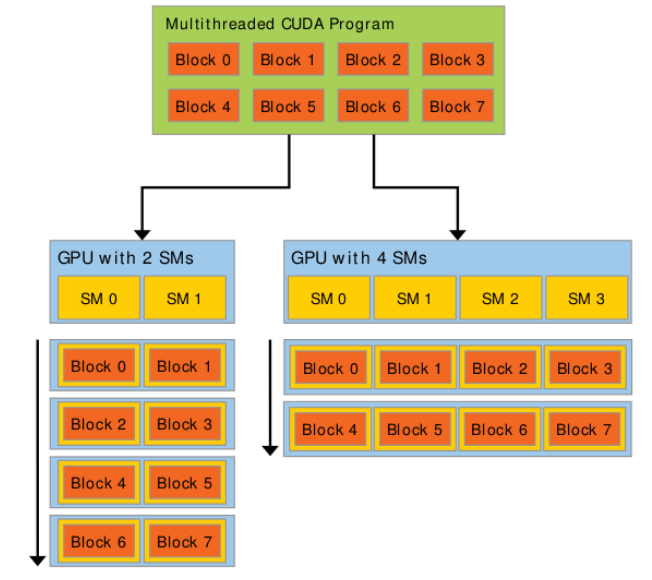
\includegraphics[width=0.8\textwidth]{images/cudaSMs.png}
		\caption{GPU scalability.}
		\label{fig:cudaSM}
	\end{figure}
	Indeed, \textit{each block of threads can be scheduled on any of the available Streaming Multiprocessors within a GPU, in any order, concurrently or sequentially}, such that a compiled CUDA program can execute on any number of SM, as illustrated by Figure \ref{fig:cudaSM}, and only the runtime system needs to know the physical multiprocessor count.
	This programming model scales on the number of multiprocessors and memory partitions\cite{cudaguide}. 
	
	We'll see in next \hyperref[sect:CUDAcpp]{section} further details on CUDA programming model, especially the extensions for C/C++ since, in this thesis, we used CUDA C++.
	
\subsection{Copy engines and Memory organization}
	On all operating systems that run CUDA, host memory is virtualized. The operating system component that manages virtual memory is the \textit{Virtual Memory Manager} (VMM), it provides services to hardware drivers, in order to facilitate direct access of host memory by hardware.\\
	In modern computers, many peripheral, as GPUs, can read or write host memory using a facility known as \textbf{\textit{Direct Memory Access}} (\textbf{DMA}). It avoids a data copy and enables the hardware to operate concurrently with the CPU\footnote{Furthermore hardware may achieve better bus performances over DMA.}.\\
	To facilitate DMA, operating system VMMs provide a service named \textit{page-locking}. Page-locked memory is ineligible for eviction and its physical addresses cannot change. Once memory is page-locked, drivers can program their DMA hardware to reference the physical addresses of the memory.
	Memory that isn't page-locked is known as \textit{pageable}, otherwise it's defined as \textbf{\textit{pinned}} memory\footnote{It's called \textit{pinned} since its physical addresses cannot be changed by the OS.}.\\
	We'll see that \textbf{\textit{host pinned memory}}\footnote{To be precise page-locked memory and CUDA's pinned aren't really the same thing: pinned memory, registered by CUDA, is mapped for direct access by the GPU; ordinary page-locked memory is not.}, with respect to the GPUs, is generally coupled with CUDA streams and it represents a page-locked portion of host memory, set up for DMA by the current CUDA context\cite{cudahandbook}.\\	
	We'll see in Subsection \ref{subs:streams} CUDA Streams and we'll see that they are linked to DMA for another reason.
	In particular, an important DMA mechanism is the so called \textbf{\textit{copy engine}}. \\
	DMA allows the transfer of data between host and device, while eventually a kernel is executing on the GPU.
	In older GPU architectures there was a single copy engine, while in newer there are usually two.
	The benefit of dual copy engines, coupled with the fact that PCIe\footnote{\textit{Peripheral Component Interconnect Express}, abbreviated as PCIe, is a high-speed serial computer expansion bus standard, designed to replace the older PCI.} is a full duplex interconnection, allows to perform more operations simultaneously, for example:
	\begin{itemize}
		\item do a memory copy from device to host;
		\item Run kernel that operates on available data in memory;
		\item do another memory copy from host to device.
	\end{itemize}
	\begin{figure}[H]
		%\vspace*{-2.4cm}
		\centering
		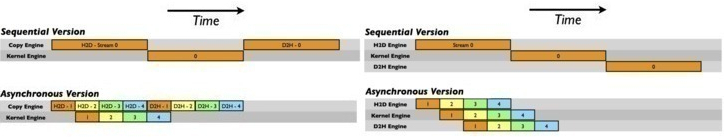
\includegraphics[width=\textwidth]{images/copy-engine.jpg}
		\caption{Comparison between one and two copy engines, using default (above) and non-default CUDA streams (below).}
		\label{fig:copyengines}
	\end{figure}
	In the ideal case, with two copy engines the data copies should be completely overlapped by kernel execution, i.e. the transfers overheads are hidden by the kernel time\footnote{We'll see what overlapping really means and how it's implemented in subsection \ref{subs:streams}}.\\
	With a single copy engine, instead, first and last steps above cannot run concurrently\footnote{Note that the simultaneous upload/download of large amounts of data across PCIe can use up a significant portion of available system memory bandwidth.}\cite{cudahandbook,custreamsblog}.\\
	In Figure \ref{fig:copyengines}, starting from the top, we have a comparison between the cases of: memory copies and kernel executions completely serial; one memory copy and kernel execution overlapping (one copy engine); two memory copies and kernel execution overlapping (two copy engines).\\
		
		
	To maximize performance, CUDA uses different types of memory, depending on the expected usage.\\
	As mentioned before, host memory refers to the memory attached to the CPU(s) in the system. Device memory is attached to the GPU and accessed by a dedicated memory controller and data should be copied explicitly\footnote{A new CUDA functionality, called \textit{Unified Memory} allows to abstract both device and host memories as if they are a unique memory, this avoids the use of explicit copies between host and device memory. However this feature wasn't used in this work, as it wasn't suitable to allow tests and measures we needed to perform in experiments. } between host and device memory in order to be processed by the GPU.\\
	Device memory can be allocated and accessed in different of ways:
	\begin{itemize}
		\item \textbf{Global memory} may be allocated statically or dynamically and accessed via pointers in CUDA kernels, which translate to global load/store instructions;
		\item \textbf{Constant memory} is read-only memory accessed via different instructions that cause the read requests to be serviced by a cache hierarchy, optimized for broadcast to multiple threads;
		\item \textbf{Local memory} contains the stack, that is local variables that cannot be held in registers, parameters, and return addresses for subroutines;
		\item \textbf{Texture memory} (in the form of CUDA arrays) is accessed via texture and surface load/store instructions; like constant memory, read requests from texture memory are serviced by a separate cache that is optimized for read-only access\cite{cudahandbook}.
	\end{itemize}
	\begin{figure}[t]%[H]
		\vspace*{-1cm}
		\centering
		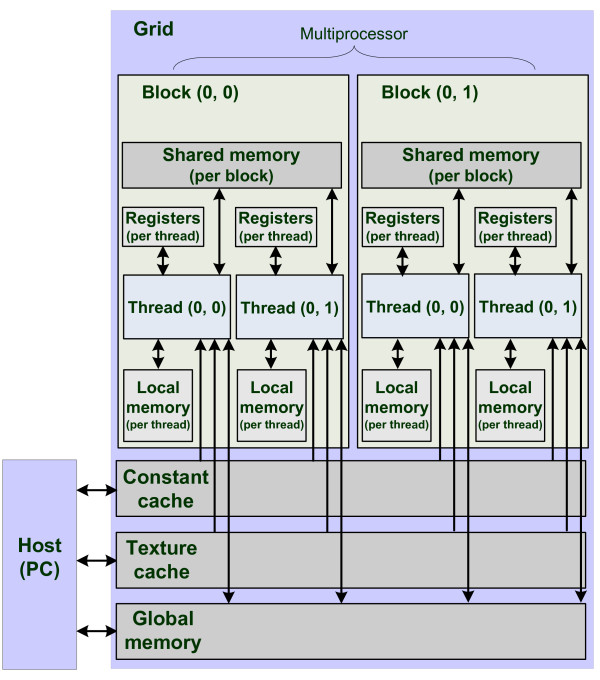
\includegraphics[width=0.7\textwidth]{images/Memory-model-CUDA-memory-hierarchy.jpeg}
		\caption{CUDA memory hierarchy and SM organization.}
		\label{fig:memhierarchy}
	\end{figure}
	Shared memory is an important type of memory in CUDA that is not supported by device memory. Instead, it is an abstraction for an on-chip memory that can be used for fast data interchange between threads within a block, has much higher bandwidth and lower latency than local and global memory\cite{cudabestpractices}. Physically, shared memory comes in the form of built-in memory on the SM.\\
	In Figure \ref{fig:memhierarchy}
	In this work we mainly exploited Global memory, it is the main abstraction by which CUDA kernels read or write device memory.\\
	The device pointer base resides in the device address space, separate from the CPU address space used by the host code in the CUDA program. As a result, host code in the CUDA program can perform pointer arithmetic on device pointers, but they may not dereference them.
	CUDA kernels can read or write global memory using standard C semantics\cite{cudahandbook}. 
	

	
\section{CUDA C/C++}
\label{sect:CUDAcpp}
	Here we'll briefly introduce main concepts behind the CUDA programming model, by outlining how they are exposed in C/C++.
	Especially we'll show important notions about features involved in this project and how/why these were included.


\subsection{Kernels} 
\label{subs:ker}
	CUDA C allows to define particular C functions, called \textbf{\textit{kernels}}, when called, the code is executed N times in parallel by N different CUDA threads, instead of executing only once, like it happens in regular C functions\cite{cudaguide}.
	
	A kernel code is defined using the \texttt{\_\_global\_\_} declaration specifier. The number of CUDA threads that will execute the kernel for a given call is specified using this special \textit{execution configuration} syntax: 
	\texttt{<<<...>>>}.\\
	Each thread executing the kernel is given a unique thread ID, accessible within the kernel through the built-in \texttt{threadIdx} variable\cite{cudaguide}.\\
	\begin{wrapfigure}{l}{0.58\textwidth}
		\raggedleft
		
		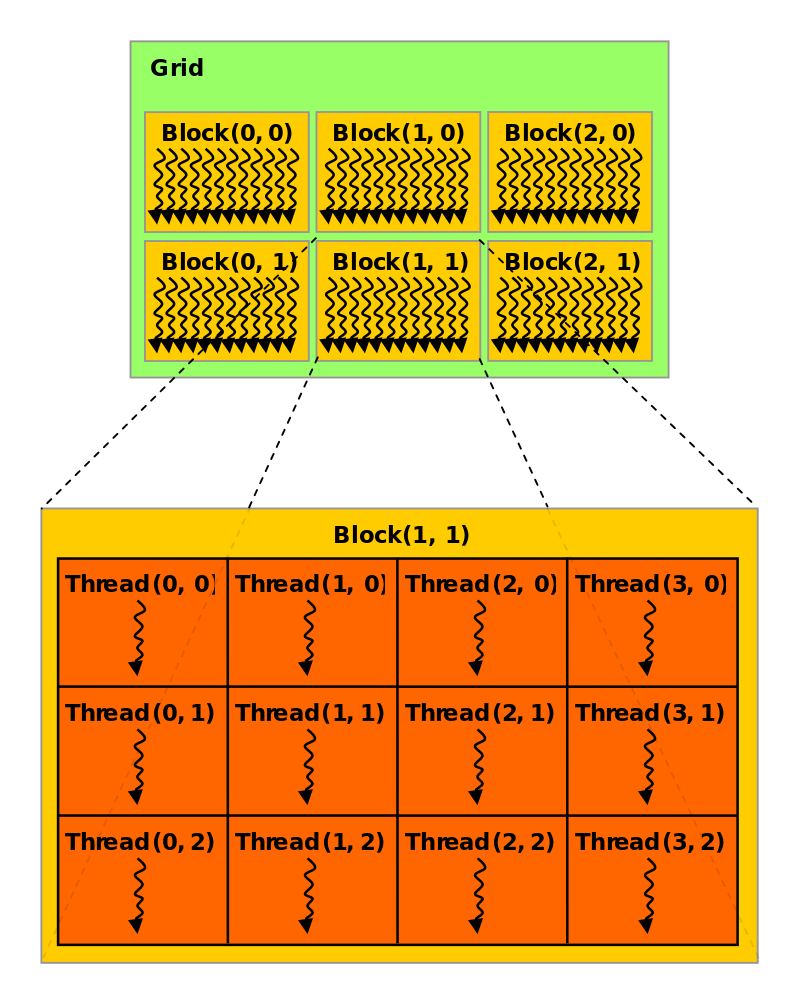
\includegraphics[width=0.58\textwidth]{images/gridblocks.png}
		\caption{Grid/Block organization: above a Grid formed by Blocks; below a Block formed by Threads.}
		\label{fig:gridblock}
	\end{wrapfigure}

\subsection{Thread Hierarchy}  
\label{subs:thrhierarchy}
	In practice \texttt{threadIdx} is a 3-component vector, so that threads can be identified using either one, or two, or three dimensional thread index.
	In turn these threads will form	either one, or two, or three dimensional block of threads, called a
	\textbf{\textit{thread block}}.
	This provides a way to invoke computation across the elements in domains such as a vectors, matrices, or volumes.
%The index of a thread and its thread ID relate to each other in a straightforward way:
%\begin{itemize}
%	\item For a one-dimensional block, they are the same; 

%	\item for a two-dimensional block of size \((D_{x} ,	D_{y}) \space \rightarrow \space\)  a thread of index \((x, y)\) has \(threadID = (x + y \cdot D_{x} );\)

%	\item for a three-dimensional block of size \((D_{x} ,	D_{y} ,	D_{z}) \space \rightarrow \space\)  a thread of index \((x, y, z)\) has \(threadID = (x + y \cdot D_{x} + z \cdot D_{x} \cdot D_{y});\)
%\end{itemize}
	There is a limit to the number of threads per block, since \textit{all threads of a block are expected to reside on the same processor core and must share the limited memory resources of that core}. On current GPUs, and on the two we worked on, a thread block may contain up to 1024 threads\footnote{see Table \ref{tab:gpuspecs} for limits in the machines we used.}.\\
	However, a kernel can be executed by multiple equally-shaped thread blocks, so that\\
	\(Total\  number\ of\ threads = \#threadsPerBlock \cdot \#blocks\)\\	 
	Blocks in turn are organized into either one, or two, or three dimensional \textit{\textbf{grid of thread blocks}} as illustrated by Figure \ref{fig:gridblock}.	
	So, the number of blocks in a grid is usually dictated by the size of the data being processed or the number of processors in the system.
	The number of \textit{threads per block} and the number of \textit{blocks per grid} specified in the 	\texttt{<<<...>>>} syntax can be of type \texttt{int} or \texttt{dim3}.\\
	The dimension of the thread block, block index and thread index are accessible within the kernel through the respective built-in variables: \texttt{blockDim}, \texttt{blockIdx}, \texttt{threadIdx}\cite{cudaguide}.

\subsection{CUDA Streams}
\label{subs:streams} 
CUDA enables fine-grained concurrency, with hardware facilities that enable threads to closely collaborate within blocks, using a combination of shared memory and thread synchronization.\\
But it also has hardware and software facilities that enable more \textit{coarse-grained concurrency}\cite{cudaguide}: 
\begin{itemize}
	\item \textit{CPU/GPU concurrency}. Since they are separate devices, the CPU and GPU can operate independently of each other;
	\item \textit{Memcpy/kernel processing concurrency}. For GPUs having one or more copy engines, \(host \leftrightarrow device\) \texttt{memcpy} can be performed while the SMs are processing kernels;
	\item \textit{Kernel concurrency}. SM, in 2.x compute capability and later hardware, can run up to 4 kernels in parallel;
	\item \textit{Multi-GPU concurrency}. For problems with enough computational density, multiple GPUs can operate in parallel.
\end{itemize}
  CUDA streams enable these types of concurrency, but we're interested in the first three types listed above.\\
  Within a given stream, operations are performed in sequential order, but operations in different streams may be performed in parallel.\\
  CUDA events complement CUDA streams by providing the synchronization mechanisms needed to coordinate the parallel execution enabled by streams. CUDA events may be used for CPU/GPU synchronization, for synchronization between the engines on the GPU, and for synchronization between GPUs.\\
  They also provide a GPU-based timing mechanism that cannot be perturbed by system events such as page faults or interrupts from disk or network controllers \cite{cudahandbook,cudaguide}. \\\\
  %
%
	\textbf{Overlap of Data Transfer and Kernel Execution}\\
	Some devices can perform an asynchronous memory copy to or from the GPU concurrently with kernel execution. 
	It's possible to query this capability by checking the \texttt{asyncEngineCount} device property\footnote{ See \textit{Device Enumeration} in Table \ref{tab:gpuspecs}, for both of our machines, from the \textit{deviceQuery}, we get 2 copy engines.}, which is greater than zero for devices that support it.
	When host memory is involved in the asynchronous copy, it must be \textit{\textbf{page-locked}} to possibly achieve a kernel-copy overlap\cite{cudastrandconcurr}.
	%In particular some devices, of compute capability 2.x and higher, can overlap copies to and from the device. Applications may query this capability by checking the \texttt{asyncEngineCount} device property (see Device Enumeration), which is equal to 2 for devices that support	it \footnote{This is the case for both of our machines. \\ See the last line of \texttt{deviceQuery} in Table \ref{tab:gpuspecs}}. 
	%\Large \textbf{Streams}\normalsize\\
	Applications manage the concurrent operations described above through \textbf{CUDA streams}.\\
	A stream is a sequence of commands (possibly issued by different host threads) that execute in order. On the other hand, a stream may execute its commands out of order or concurrently with respect to another; this behavior is not guaranteed and	should not be relied upon for correctness (e.g. inter-kernel communication is undefined)\cite{cudaguide,custreamsblog}.\\
	A brief code example:
	\begin{lstlisting}[caption={CUDA Strams creation}]
	cudaStream_t stream[2];
	for (int i = 0; i < 2; ++i)
		cudaStreamCreate(&stream[i]);
	float* host;
	cudaMallocHost(&host, 2 * size); //host mem allocation must be pinned
	\end{lstlisting}	
	
	On each of these CUDA streams will be issued a sequence of commands. In the following code sample we have one memory copy \(host \rightarrow device\), one kernel launch, and one memory copy \(host \leftarrow device\):
	\begin{lstlisting}[caption={CUDA Strams and Async example}]
	for (int i = 0; i < 2; ++i) {
		cudaMemcpyAsync(inputDev+i*size, host+i*size, size, cudaMemcpyHostToDevice, stream[i]);
		MyKernel<<<BLOCK,GRID,0,stream[i]>>>(outputDev+i*size, inputDev+i*size, size);
		cudaMemcpyAsync(host+i*size, outputDev+i*size, size, cudaMemcpyDeviceToHost, stream[i]);
	}
	...	
	for (int i = 0; i < 2; ++i)
		cudaStreamDestroy(stream[i]);
	\end{lstlisting}
	
	Each stream copies its portion of input array \texttt{host} to array \texttt{inputDev} in device memory, calls \texttt{MyKernel()} to process computations on \texttt{inputDev} and copies
	the result \texttt{outputDev} back to the same memory portion, i.e. \texttt{host}. Note that \texttt{host} must point to page-locked host memory for any possible overlap to occur.\\
	Streams are finally released by calling \texttt{cudaStreamDestroy()}.


\subsection{\texttt{nvcc} compiler}
	To compile the CUDA C++ code it is necessary to use a special compiler, included in CUDA Toolkit, that is \texttt{nvcc}.\\
	The CUDA compiler driver hides the details of CUDA compilation from developers. It accepts a range of conventional compiler options, for example for the project we could define macros or include library paths.
	All non-CUDA compilation steps are forwarded to a C++ host compiler that is supported by \texttt{nvcc}. 
	Source files compiled with \texttt{nvcc} can include a mix of host code and device code\cite{nvccdoc}.\\ \texttt{nvcc}'s basic workflow consists in separating device from host code and then:
	\begin{itemize}
		\item compiling the device code into an assembly form (PTX code) and/or binary form (cubin object), \item and modifying the host code by replacing the \texttt{<<<...>>>} syntax introduced in Kernels\footnote{See  \hyperref[subs:ker]{subsection 2.3.1}} by the necessary CUDA C runtime function calls, to load and launch each compiled kernel from the PTX code and/or cubin object.
	\end{itemize}
	The modified host code is output either as C code that is left to be compiled using another tool, or as object code directly by letting \texttt{nvcc} invoke the host compiler during the last compilation stage.
	Applications can then either link to the compiled host code (most common case), or ignore the modified host code (if any) and use the CUDA driver API to load and execute the PTX code or cubin object\cite{nvccdoc}.\\
	This compiler can be used almost the same way as a classic \texttt{gcc}, for example:
		
	\texttt{nvcc -std=c++14 -g -G -o exec source.cu}\\
	This is an example that compiles the file \texttt{source.cu} in the executable file \texttt{exec}, keeping debug information with \texttt{-g -G} flags.
	Here we present compiler versions installed in our two machines:	
	\begin{itemize}
		\item \textbf{Tesla P100}\\
		\texttt{nvcc}: NVIDIA® Cuda compiler driver, release 10.1, V10.1.168			
		
		\item \textbf{Tesla M40}\\
		\texttt{nvcc}: NVIDIA® Cuda compiler driver, release 10.1, V10.1.105
	\end{itemize}

	\subsection{\texttt{cuda-gdb} debugger}
	\texttt{CUDA-GDB} is the NVIDIA tool for debugging CUDA applications (available on Linux). It is an extension to the x86-64 port of GDB, the GNU Project debugger\cite{cudagdbdoc}.\\
	\texttt{CUDA-GDB} main features are:
	\begin{itemize}
		\item it provides an environment that allows simultaneous debugging of both GPU and CPU code within the same application;
		
		\item as programming in CUDA C is an extension to C programming, debugging with CUDA-GDB is an extension to debugging with GDB, so the existing GDB debugging features are present for debugging the host code (additional features have been provided to support CUDA device code);	
		
		\item it allows to set breakpoints, to single-step CUDA applications, and also to inspect and modify the memory and variables of any given thread running on the hardware;
		
		\item it supports debugging all CUDA applications, whether they use the CUDA driver API, the CUDA runtime API, or both.
		
		\item it supports debugging kernels that have been compiled for specific CUDA architectures, but also supports debugging kernels compiled at runtime, referred to as just-in-time (JIT) compilation\cite{cudagdbdoc}.
	\end{itemize}	
	\texttt{CUDA-GDB} was used to debug all compiled source files, both \texttt{.cu} and \texttt{.cpp} .
	Mainly it was really helpful in this project to step device code, inspect runtime errors thrown by CUDA API calls and check for errors in the code inside our kernels.





\section{Profilers}	
	NVIDIA profiling tools were useful to optimize performances of our CUDA applications.\\
	We used two different versions, that will be showed in the following sections.
		
	\subsection{\texttt{nvprof}}
	The\texttt{nvprof} provides a tool to collect and view profiling data from the command-line.
	\texttt{nvprof} was added to CUDA Toolkit with CUDA 5. It is a command-line profiler, so it's a GUI-less version of the graphical profiling features available in the NVIDIA Visual Profiler.\\
	The \texttt{nvprof} profiler enables the collection of a timeline of CUDA-related activities on both CPU and GPU, including kernel execution, memory transfers, memory set and CUDA API calls and events or metrics for CUDA kernels.\\
	After all data is collected, profiling results are displayed in the console\footnote{The textual output of the profiler is redirected to \texttt{stderr} by default.} or can be saved in a log file for later viewing \footnote{Or for later import into either \texttt{nvprof} or the \texttt{NVIDIA Visual Profiler}.}.\\
	\texttt{nvprof} operates in different modes: \textit{Summary Mode}, \textit{GPU-Trace and API-Trace Modes}, \textit{Event/metric Summary Mode} and  \textit{Event/metric Trace Mode}\cite{profilersguide, nvprofarticle}.\\	
	For our purposes we used only \textit{Summary Mode}, this is the default operating mode, where we have a single result line for each kernel function and each type of CUDA memory copy performed by the application (for each operation type are shown total, maximum, minimum, average times and number of calls)\cite{profilersguide}.
	
	We used it, in some situations, as a quick check, for example we exploited it to see if the application wasn't running kernels on the GPU at all, or it was performing an unexpected number of memory copies, etc.
	To this aim it's enough to run the application with
	
	\texttt{nvprof ./myApp arg0 arg1 ...}\\
	Given that we even wanted to consult profiling results whenever it was necessary, we used \texttt{--log-file} option to redirect the output to files for deferred examination. \\
	\texttt{nvprof} revealed peculiarly suitable for remote profiling. That's because of the fact command line is faster to check and save an application profiling.
	  
	\subsection{NVIDIA Visual Profiler}
	The \texttt{NVIDIA Visual Profiler}, introduced in 2008, is a performance profiling tool providing visual feedback for optimizing CUDA C/C++ applications.
	
	The Visual Profiler displays a timeline of an application's activity on both the CPU and GPU to make performance improvement, it analyzes the application to detect potential bottlenecks, using graphical views, that allow to check memory transfers, kernel launches, and other API functions on the same timeline \cite{profilersguide}.\\
	 
	\texttt{Visual Profiler} was also used in developing phase, to check if the application gave overlapping, or to see if we could hide as much as possible data transfers\footnote{We'll see in detail the Overlapping topic and how it was managed in \hyperref[chap:logic]{Chapter 3}.}, even though sometimes it may happen that profilers introduce some sampling synchronization, giving some little imprecision in visual results.

	
\section{Visual Studio Code}
	Visual Studio Code is an open-source code editor by Microsoft that also runs on Linux Operating Systems. It includes support for debugging, embedded Git control and GitHub, syntax highlighting, intelligent code completion, snippets, and code refactoring \footnote{Documentation: https://docs.microsoft.com/it-it/dotnet/core/tutorials/with-visual-studio-code \\ 
		Website: https://code.visualstudio.com/}.\\
	Since it's customizable we could add C++ and CUDA editor extensions, furthermore an SFTP extension allowed us to quickly upload/download files from remote machines. 	
	
	
\section{Tests, Result gathering, Plots}
	Some other additional tools have been used in this project.
	In particular we needed:
	\begin{itemize}
		\item to serially run executions of our applications, possibly varying input dataset on interest values;
		\item to group all results on text files;
		\item to implement a script that, from results on text files, computed average time measures, speedups, other interest metrics and generate plots on important values.
	\end{itemize}
	
	\subsection{Bash scripts}
	\label{subs:bash}
	Bash (\textit{Bourne-Again SHell}) is the shell, or command language interpreter, for the GNU operating system; the latter provides other shells, but Bash is the default  one\footnote{https://www.gnu.org/software/bash/manual/}. 
	
	\textbf{\texttt{Bash scripts}} were needed to implement tests, that run more executions of a certain CUDA application, also varying input dataset.
	We programmed bash scripts (\texttt{.sh}) tests to contain several command as compile a certain CUDA application, run many times the related executable, profile it with \texttt{nvprof} and so on.\\
	Below we give a brief example on how we used bash scripts to implement tests:
	\begin{lstlisting}[caption={Tests on bash scripts example},language=bash]
	#!/bin/bash
	
	...			
	let GPU=3
	let B=1024
	let nTests=4

	Miters=(10000 400000 800000)
	Ns=(57344 114688 229376 458752 917504 1835008)
		
	#parameters: deviceID, BLOCK, N_elements, M_iterations, cuStr[bool], strNum
	make cleandplow
	echo -e "${BLUE}compiling stream...${NC}"	
	make streamlow
	
	echo ***STREAM_LOW_NOSTREAM_test***
	for N in "${Ns[@]}"
	do			
		for m in "${Miters[@]}"
		do	
			echo sizeN = $N elements, kerM = $m , CUstreams = 0 
			echo -n execIndex = 
			
			for((j=0; j<nTests; j+=1));
			do
				echo -n "$j , "
				./bin/streamlow.out $GPU $B $N $m 0 0 >> ./results/dev_cos_dp_stl.txt
			done
			echo -ne "$nTests \n"			
			nvprof --log-file ./profiling/dev_str_low$N-$m-$B-0.txt ./bin/streamlow.out $GPU $B $N $m 0 0 >> ./results/dev_cos_dp_stl.txt
		done
	done
	\end{lstlisting}
	Here, for example, the code is setting up all input data set, it compiles the code with the \texttt{streamlow} \texttt{Makefile} rule into an executable, then it loops over all data sets to run the executable in each configuration.\\
	Here we can see that each setting is repeated more times (to allow outliers elimination) and one of those executions is performed via the \texttt{nvprof} profiler, in any case all executions outputs are redirected to \texttt{.txt} files for later consultation.
	
	
	\subsection{Python scripts}
	As Python \footnote{The Python version used to compile, on local host, our scripts is: Python 2.7.6.\\ Documentation: https://docs.python.org/2/} has dynamic typing, together with its interpreted nature, it's an ideal language for scripting and rapid application development.
	
	In the case of this work was most useful to quickly implement a result filter: given text files with time measures, we computed averages and some speedups. \\
	Furthermore we implemented a script to generate some plots on averages and speedups, exploiting the library \texttt{matplotlib}\footnote{https://matplotlib.org/}.\\
	Below we show a part of the code to compute speedups and generate some plots:\\
	\begin{lstlisting}[caption={Portion of speedup and plots Python script}, language=python]
	def main():		
		res_path = "./output/"+sys.argv[1]+"/"
		for file in os.listdir(res_path):
			if file.endswith("avgs.csv"):
				f=os.path.join(res_path, file)				
				resType=file[0:3]
				if resType=="cos":
					dataPar,zeroStream,threeStream,coresStream = getDividedData(dpCosTest,strCosTest,f)	
				elif resType=="mat":
					...
				...				
				zeroThree,zeroCore,coreDp = getSpeedup(zeroStream,threeStream,coresStream,dataPar)				
				##write speedup to CSV##
				csvPath=res_path+resType+"_sp.csv"		
				with open(csvPath,  "wb") as fcsv:
					writer = csv.writer(fcsv) 					
					printSpToCSV("Tseq/T3",zeroThree,resType,writer) 
					printSpToCSV("Tseq/Tsm",zeroCore,resType,writer)
					printSpToCSV("Tsm/Tdata",coreDp,resType,writer)	
				#########
				# Plots #
				#########
				# Completion Time
				launchPlots(resType,zeroStream,"Zero Streams")
				launchPlots(resType,threeStream,"Three Streams")
				launchPlots(resType,coresStream,"#SM Streams")
				# Speedup	
				if sys.argv[1]=="M40":
					streamNums=[1,3,24]
				elif sys.argv[1]=="P100":
					streamNums=[1,3,56]				
				
				if resType=="cos":
					plotSpeedup(streamNums, zeroStream, zeroThree, zeroCore, resType, cosN, cosM)	
				elif resType=="mat":
					plotSpeedup(streamNums, zeroStream, zeroThree, zeroCore, resType, matNum, matSize)		
				....			
	#########################
	# Speedup plot function #
	#########################
	def plotSpeedup(streamNums,zeroStream, zeroThree , zeroCore, resType,param1,param2):				
		title="Speed Up"		
		title=title.upper()				
		plt.figure(figId)
		plt.plot([0]+streamNums, [0]+streamNums, marker='.',label='Ideal speed up',linestyle='--')
		.....
	
		if resType=="cos":
			indexes=[0, param2-1, len(zeroCore)-param2, len(zeroCore)-1]
			for i in indexes:
				tmp=[1.0, zeroThree[i][2],zeroCore[i][2]]
				lblLine=str(zeroThree[i][0]) +" - "+str(zeroCore[i][1])
				plt.plot(streamNums, tmp, '-', label = lblLine, marker=markers[j], linestyle='-', linewidth=lineW, alpha=alphaVal)
				
				lineW+=0.5
				alphaVal-=0.2
				j+=1
		.....
		
		plt.xticks(streamNums)
		plt.yticks(streamNums)
		plt.legend(loc="upper left")
		plt.grid(axis='both')
		plt.ylabel("Speedup")
		plt.xlabel("#CUDA Streams")
		plt.show()
		figId+=1
	\end{lstlisting}
	
	The code above starts in function \texttt{main()}, it initially reads from a \texttt{.csv} file the average time measures for all different executions, given by one of the three applications we tested.\\
	Then in the main we split times of all execution types (e.g. zero, three or number of SM amount of CUDA streams used). At this point code has what it needs to get speedups\footnote{We'll see in Chapter \ref{chap:experim} all types of speedup we compute, how and why.} in \texttt{getSpeedup}, this function computes speedup (from input parameters) then it saves results in a \texttt{.csv} file and output them to the main function too.\\
	Finally the main calls the functions that provide completion time and speedup plots, respectively called \texttt{launchPlots} and \texttt{plotSpeedup}. The latter plots all different speedups, given by the different input data sets of executions, compared with the line of ideal speedup.\\
	Note that the mean values of time measures (used as input of the speedup/plot script above) are in turn generated by another python script.
	


    %\section{Project Logic}
\chapter{Project Logic}
\label{chap:logic}
%\pagenumbering{arabic}

The reasoning in this work started by considering the characters of a problem that is recognizable in a Farm parallel pattern.
Then the study moved to consider how a GPU works, main architectural characteristics and facing its data parallel nature.
Next we had to think how to "merge" two such different behaviors, in order to reach reasonable performances \footnote{About expected performances see \hyperref[sect:overallLogic]{Section 3.3} and \hyperref[sect:tunings]{Section 3.4} for more clarifications}, i.e. almost competitive with a classic data parallel problem.
Finally, once the main idea behind the development was clear, we had to make some tunings.
All of these steps will be shown in detail in next sections.

\section{Streaming Parallelism: Farm pattern}
Stream parallel patterns describe problems exploiting parallelism among computations relative to
different, independent data items appearing on the program input stream.
Each independent computation end with the delivery of one single item on the program output stream.\\
We focused on farm pattern, modeling embarrassingly parallel stream parallelism. 
For example, consider the correspondent skeleton:\\
\texttt{let rec farm f =\\
	function\\
	EmptyStream -> EmptyStream\\
	| Stream(x,y) -> Stream((f x),(farm f y));;\\
	}
	
whose type is\\
\( farm :: (\alpha \rightarrow \beta) \rightarrow \alpha stream \rightarrow \beta stream \)\\

\textit{The parallel semantics, associated to the higher order functions, states that the computation of any items appearing on the input stream is performed in parallel}\\

In the farm case, according to the parallel semantics a number of parallel agents computing function \(f\) onto input data items equal to the number of items appearing onto the input stream could be used. This is not realistic, however, for two different reasons:

\begin{enumerate}
	\item items in the stream do not exist all at the same time. A stream is not a vector.
	Items of the stream may appear at different times. Actually, when we talk of consecutive items \(x_{i}\) and \(x_{i+1}\) of the stream we refer to items appearing onto the stream at times \(t_{i}\) and \(t_{i+1}\) with \(t_{i} < t_{i+1}\). As a consequence, it makes no sense to have a distinct parallel agent for all the items of the input stream, as at any given time only a fraction of the input stream will be available.
	
	\item if we use an agent to compute item \(x_{k}\), presumably the computation will end at some
	time \(t_{k}\). If item \(x_{j}\) appears onto the input stream at a time \(t_{j} < t_{k}\) this same agent
	can be used to compute item \(x_{j}\) rather than picking up a new agent. \\
\end{enumerate}
This is why the parallelism degree of a task farm is a critical parameter: a small parallelism degree doesn't exploit all the parallelism available (thus limiting the speedup), while a large parallelism degree may lead to inefficiencies as part of the parallel agents will be probably idle most of time \cite{spm}.\\

%In some skeleton frameworks, therefore, the parallelism degree is given as a parameter of
%the skeleton. The task farm skeleton is therefore defined as an high order function having
%(also) an integer as a parameter. This parameter represent their intended parallelism degree
%of the implementation of the skeleton. 
%However it has no effect on the “function” computed by the skeleton. It has only effect on the “parallel semantics” metadata.
%A task farm skeleton with a parallelism degree parameter may therefore be defined with
%the high order function
%let rec farm f n:int =
%function
%EmptyStream -> EmptyStream
%| Stream(x,y) -> Stream((f x),(farm f y));;
%whose type is now
%f arm :: (α → β) → int → α stream → β stream
%with the parallel semantics defined as follows:
%the computation of consecutive items of the input stream is performed in parallel on
%n parallel agents.
%These non functional parameters of skeletons generated quite a huge debate within the skeleton community. 
%On the one side, as skeletons pretend to abstract all the aspects related
%to parallelism exploitation, non functional parameters such as the parallelism degree should
%not be left under application programmer responsibility. Rather, they should be properly
%handled by the skeleton implementation, possibly being computed using some performance
%model of the skeleton (see Chap. 5). On the other side, such parameters can be used by
%expert programmers to express the fact they want to use exactly that amount of resources.
%As an example, they may want to experiment different parallelism degrees according to the
%type of the execution constrains of the applications. If the computation of the results is
%not urgent, smaller parallelism degrees may be required, whereas, in case of very urgent
%computations, higher parallelism degrees may be asked through non functional parameters.
%Consistently with the idea a skeleton is a programming abstraction hiding all the details
%related to parallelism exploitation pattern implementation, we agree on the idea that the
%better choice is to leave to the skeleton implementation the management of all the non
%functional skeleton parameters. In case the programmer is allowed to provide such kind of
%parameters, they will be only taken as loose requirements on the execution of the skeleton:
%the implementation of the skeleton will try to accommodate user requests, but in case
%the implementation could figure out the requests are not reasonable or that better choices
%could be made, these better choices will be actually taken and the user will be consequently
%informed.


%3.2.1
%Stream modelling
%An alternative way of defining stream parallel algorithmic skeletons assumes pipeline and
%farm just operate on a global input stream of data to produce a global stream of results. In
%this case, we may define pipelines and farms with much simpler higher order functions that
%do not operate on streams, actually, and then use these functions as parameters of another
%higher order function implementing stream parallelism. In this case, the pipeline skeleton
%will basically correspond to functional composition:
%let pipeline f g =
%function x -> (g (f x));;
%while task farm skeleton corresponds to identity:
%let farm f =
%function x -> (f x);;
%The higher order function taking care of exploiting parallelism can then be defined as follows:
%let rec streamer f x =
%match x with
%EmptyStream -> EmptyStream
%| Stream (v,s) -> Stream ((f v), (streamer f s));;
%such that, to define the filter/recognize program defined in Sec. 3.2 we can now write:
%let main =
%streamer (pipeline filter recognize);;
%Clearly, the parallel semantics associated to skeletons changes in this case, with respect
%to the parallel semantics we had when pipeline and farms actually processed streams. A
%parallel semantics is only associated to the streamer function as:
%the processing of independent input stream data items is performed in parallel
%whereas pipeline and farm have do not have associated any kind of parallel semantics.
%This way of modelling stream parallelism corresponds to the idea of structuring all stream
%parallel applications as farms 51 with more coarse grain computations as functional param-
%eter.
%Again, consider the filter/recognize example. Let’s suppose that the recognize phase is
%much more computationally expensive with respect to the filter phase. Using the explicit
%stream handling versions of pipeline and farm skeletons, we would write the program as
%let main =
%pipeline (filter) (farm recognize);;
%51 recall the parallel semantics previously given for the farm and look at the analogies in between the streamer
%function and the former definition of the farm higher order function58
%ALGORITHMIC SKELETONS
%Recalling the parallel semantics of these skeletons we can easily understand that given a
%stream with data items x 1 , . . . , x m (with x i appearing on the stream after x i−k for any k)
%the computations of
%recognize(y i ) recognize(y i+k )
%(being y i = f ilter(x i )) happen in parallel, as well as the computations of
%recognize(y i ) f ilter(x i+k )
%If we use the alternative modelling of stream parallelism described in this section, the
%program instead is written as
%let main =
%streamer (pipeline filter recognize);;
%and in this case the only computations happening in parallel are the
%recognize(f ilter(x i )) recognize(f ilter(x i+k ))


%3.3 A SIMPLE SKELETON FRAMEWORK
%Although different programming frameworks based on skeletons have been developed that
%sport each different algorithmic skeletons, a subset of common skeletons may be found in
%most of these frameworks. These common subset contains skeletons from three different
%classes of skeletons: stream parallel skeletons, data parallel skeletons and control parallel
%skeletons.
%3.3.1
%Stream parallel skeletons
%Stream parallel skeletons are those exploiting parallelism among computations relative to
%different, independent data items appearing on the program input stream. Each indepen-
%dent computation end with the delivery of one single item on the program output stream.
%Common stream parallel skeletons are the pipeline and task farm skeletons, whose definition
%in terms of higher order functions and parallel semantics has already been given in Sec. 3.2.
%The pipeline skeleton is typically used to model computations expressed in stages. In
%the general case, a pipeline may have more than two stages. The restriction to two stages
%as given by the definition in Sec. 3.3.4 guarantees strong typing and the ability to define
%pipelines with more than two stages as pipelines of pipelines. Given a stream of input tasks
%x m , . . . , x 1
%the pipeline with stages
%s 1 , . . . , s p
%computes the output stream
%s p (. . . s 2 (s 1 (x m )) . . .), . . . , s p (. . . s 2 (s 1 (x 1 )) . . .)
%The parallel semantics of the pipeline skeleton ensures all the stages will execute in
%parallel. In Chap. 5 we will see that this guarantees that the total time required to compute
%a single task (pipeline latency) is closed to the sum of the times required to compute the
%different stages. Also, it guarantees that the time needed to output a new result is close to
%time spent to compute a task by the longer stage in the pipeline.A SIMPLE SKELETON FRAMEWORK
%59
%The farm skeleton is used to model embarrassingly parallel computations, instead. The
%only functional parameter of a farm is the function f needed to compute the single task.
%Given a stream of input tasks
%x m , . . . , x 1
%the farm with function f computes the output stream
%f (x m ), . . . , f ( x 1 )



We recall that the only functional parameter of a farm is the function \(f\) needed to compute the single task.
Given a stream of input tasks
\begin{center}
	\(x_m , . . . , x_1\)\\
\end{center}
the farm with function \(f\) computes the output stream
\begin{center}
	\(f ( x_m ), . . . , f ( x_1 )\)\\
\end{center}
Its parallel semantics ensures it will process the single task in a time close to the time needed to compute \(f\) sequentially \cite{spm}. %The time between the delivery of two different task results, instead, can be made close to the time spent to compute f sequentially divided by the number of parallel agents used to execute the farm, i.e. its parallelism degree.
%\cite{spm}		


\section{CPU-GPGPU: heterogeneous architecture}
The target of this project was to exploit GPGPUs high parallelism to lighten the CPU from computation intensive problems, in particular associated to the above explained Farm parallel pattern.\\
So we asked ourselves what could happen if we wanted to manage such computations on streams in a way such that:
\begin{enumerate}
	\item Input stream arrives from host side, being directly generated by CPU or acquired from a remote source;
	
	\item Items are sent from host (main memory) to the GPU (global memory);
	
	\item GPU cores apply specific computations on all items of the stream (as soon as they available in global memory);
	
	\item Finally, computed elements will be copied back to host side and will become the output stream. \\
\end{enumerate}

	In this list our main concern is about data transfer, i.e. step 2 and 4. 
	Indeed these phases introduce an overhead per se, but especially in Farm parallel pattern they can be a not negligible bottleneck.\\
	We should not forget that our input is a stream: even if elements are available with a high throughput, they come "one by one".
	In reality, as we mentioned in the previous section, we have only a part of input available at one point, so it's not realistic to have one worker per stream element.
	
	In our case we can suppose Streaming Multiprocessors to be our Farm workers, so if we don't give enough work (items) to each core we would have a resources waste.\\
	Furthermore, we surely don't want to transfer from/to GPU one element at time but, at the same time, in some way we have to keep as much as possible the nature of a Stream parallel patterns.\\	
	Thus at this point has become necessary for first to find some stratagems:
	\begin{itemize}
		\item Hide as much as we can data transfer times, both in  \(Host \rightarrow Device\)  and  \(Device \rightarrow Host\)  direction;
		\item Exploit almost completely our workers resources, in other words try to make Streaming Multiprocessors as busy as possible.
	\end{itemize}

	
	\subsection{Overlapping: Data Transfer hiding}
	In \hyperref[subs:stream]{Section 2.3.3}, we introduced CUDA Streams and we recall that they can perform asynchronous memory copies to or from the GPU	concurrently with kernel execution. 
	Since the machines we worked on both have concurrency on data copy and kernel execution and they have 2 copy engines, we exploited this capability combined with streams.\\
	In this way we wanted to achieve a situation in which we could overlap, as much as it was possible, the time it took for the GPU to execute a kernel and the time it took to transfer data back and forth.
	
	As an example see Figure \ref{fig:threeStreams} to understand a simple case with 3 CUDA Streams.
	In that diagram we can see the expected behavior of three streams, but we can extend our expectations to more than three streams, without forgetting that we can have at most 2 data transfer at the same time (given that we've two copy engines).
	
	It's important to point out that not always we can have an ideal behavior in Streams, finding a performance improvement lower than the amount we expected.
	
	Overlap amount depends on several factors: on the order in which the commands are issued to each stream, whether or not the device supports overlap of data transfer and kernel execution, concurrent kernel execution, and/or concurrent data transfers, the balancing between data transfers time and kernel executions time.\\
	Given that our GPUs supported all kind of above mentioned concurrencies, among the above factors the only that can influence in our case are the order, in which commands are issued to each stream, and the kernel/data transfer time balancing.\\
	\begin{figure}
		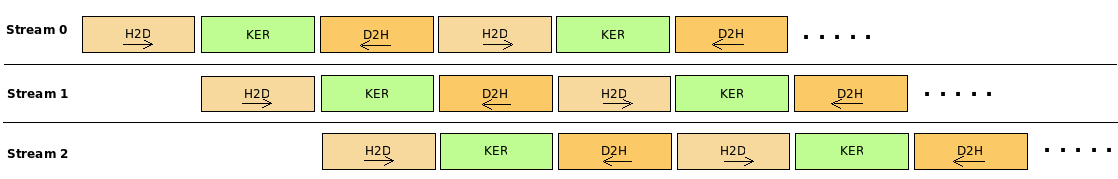
\includegraphics[width=\linewidth]{images/3Streams.png}
		\caption{Ideal behavior for 3 CUDA Streams.}
		\label{fig:threeStreams}
	\end{figure}
	We followed some useful guidelines to improve the potential for concurrent kernel execution:
	\begin{itemize}
		\item All independent operations should be issued before dependent operations;
		\item Synchronization of any kind should be delayed as long as possible.
	\end{itemize}

	For the former, we have that all operations are independent, given the Farm nature. Indeed all stream items and their computation given by workers, are independent.\\
	For the latter, we were careful to avoid \textit{Implicit synchronization}, this happens when are introduced host issued operations in-between different streams commands.\\
	Moreover we avoided all possible \textit{Explicit synchronizations} \footnote{In CUDA there are several command to force synchronization either between host and device, or between streams etc.}.
	
	Another important face of overlapping, is that we should try to balance Kernels work in such a way it's sufficient to hide the time spent in data transfers, as we quoted just above. 
	This said we can have two unfair scenarios:
	\begin{itemize}
		\item Data transfers take a small amount of time, while kernels are doing lot of computations;
		
		\item Data transfers take a big amount of time, with respect to time spent in kernel execution.
	\end{itemize}
	
	The former case may arise when we have heavy computations or \textit{"irregular kernels"}.
	By irregular we mean that any flow control instruction (\texttt{if}, \texttt{switch}, \texttt{do}, \texttt{for}, \texttt{while}) can significantly affect the instruction throughput by causing threads of the same warp to diverge; that is, to follow different execution paths.\\ 
	If this happens, the different execution paths must be serialized, increasing the total number of instructions executed for this warp. When all the different execution paths have completed, the threads converge back to the same execution path.	
	So we should avoid different execution paths within the same warp \cite{cudaguide}.\\
	% To obtain best performance in cases where the control flow depends on the thread ID, the controlling condition should be written so as to minimize the number of divergent warps. This is possible because the distribution of the warps across the block is deterministic
	% as mentioned in Section 4.1 of the CUDA C Programming Guide. A trivial example is when the controlling condition depends only on(threadIdx / WSIZE) where WSIZEis the warp size. In this case, no warp diverges because the controlling condition is perfectly aligned with the warps 
	
	
	Whilst the latter case can happen when we move an amount of data at each transfer such that it takes more time than calculations. So in this case the dominant factor will be the data transfer.	
	%So about these two scenarios we had to make some assumptions and tunings, that we will see in ********. 

	
	\subsection{Occupancy of GPU cores}
	Once we carried out the stream logic, we had to understand how to try to exploit almost every Streaming Multiprocessor at any given time.
	This means that we wanted to launch as many kernels as needed to arrive near the full \textit{\textbf{Occupancy}}.
	
	Clearly, when we start, we'll have a portion of time, a sort of "warm up" phase, where we'll have first data transfers and kernels. So we'll have a narrowed number of running kernels. 
	But as soon as we could have enough data transfers and so a lot of kernels, we would reach a workload peak on GPU.\\
	In practice, when we just said \textit{lot of kernels}, we meant a lot of small groups of items on which apply our computations, in other words this small items groups will be assigned each to a thread block.\\ Let's spend a bit to explain better what Occupancy means.\\

	To \textit{\textbf{maximize utilization}} the application should be structured in a way that it exposes
	as much parallelism as possible and efficiently maps this parallelism to the various	components of the system to keep them busy most of the time.\\
	Here main ways to maximize utilization:
	\begin{enumerate}
			\item \textbf{Application Level}
			At a high level, the application should maximize parallel execution between the host, the
			devices, and the bus connecting the host to the devices, by using \textit{asynchronous functions} calls and streams;
			
			
			\item \textbf{Device Level}
			At a lower level, the application should maximize parallel execution between the multiprocessors of a device.
			Multiple kernels can execute concurrently on a device, so maximum utilization can also be achieved by using streams to enable enough kernels to execute concurrently;
			
			
			\item \textbf{Multiprocessor Level}
			At an even lower level, the application should maximize parallel execution between the	various functional units within a multiprocessor.
			In particular, \textit{a GPU multiprocessor relies on thread-level parallelism to maximize utilization of its functional units}. 
	\end{enumerate}
	
	From the above, it's clear that occupancy is directly linked to the number of resident warps. At every instruction issue time, a warp scheduler selects a warp that is ready to execute its next instruction, if any, and issues the instruction to the active threads of the warp.\\
	The number of clock cycles it takes for a warp to be ready to execute its next instruction is called the \textit{\textbf{latency}, and full utilization is achieved when all warp schedulers always have some instruction to issue for some warp at every clock cycle during that latency period, or in other words,	when latency is completely "hidden"}. 
	
	The most common reason a warp is not ready, to execute its next instruction, is that the instruction's input operands are not available yet.\\
	If all input operands are registers, latency is caused by register dependencies, i.e., some of the input operands are written by some previous instruction(s) whose execution has	not completed yet.\\ In the case of a back-to-back register dependency (i.e., some input
	operand is written by the previous instruction), the latency is equal to the execution time of the previous instruction and the warp schedulers must schedule instructions for different warps during that time.\\
	%Execution time varies depending on the instruction, but it is typically about 11 clock cycles for devices of compute capability 3.x, which translates to 44 warps for devices of compute capability 3.x (assuming that warps 	execute instructions with maximum throughput, otherwise fewer warps are needed).
	%This is also assuming enough instruction-level parallelism so that schedulers are always able to issue pairs of instructions for each warp.
	%If some input operand resides in off-chip memory, the latency is much higher: 200 to 400 clock cycles for devices of compute capability 3.x. 
	
	%The number of warps required to keep the warp schedulers busy during such high latency periods depends on the kernel code and its degree of instruction-level parallelism. In general, more warps are required if the ratio of the number of instructions with no off-chip memory operands 	(i.e., arithmetic instructions most of the time) to the number of instructions with off-chip 	memory operands is low (this ratio is commonly called the arithmetic intensity of the program). For example, assume this ratio is 30, also assume the latencies are 300 cycles on devices of compute capability 3.x. Then about 40 warps are required for devices of compute capability 3.x (with the same assumptions as in the previous paragraph).
	Another reason a warp is not ready, to execute its next instruction, is that it is waiting at some \textit{memory fence} (\textit{Memory Fence Functions}) or synchronization point.\\ A synchronization point can force the multiprocessor to idle as	more and more warps wait for other warps in the same block to complete execution of instructions.\\
	So, having multiple resident blocks per multiprocessor can help reduce idling in this case, as warps from different blocks do not need to wait for each other at synchronization points.
	
	The \textit{number of blocks and warps residing on each multiprocessor for a given kernel call depends on the execution configuration of the call} (grid and block dimensions), the memory resources of the multiprocessor, and the resource requirements of the kernel \cite{cudaguide}.\\
	Register and shared memory are others important Occupancy variables, but we didn't focused much on them as on execution configuration.\\
%	The number of registers used by a kernel can have a significant impact on the number	of resident warps. For example, for devices of compute capability 6.x, if a kernel uses 64 registers and each block has 512 threads and requires very little shared memory, then two blocks (i.e., 32 warps) can reside on the multiprocessor since they require 2x512x64 registers, which exactly matches the number of registers available on the multiprocessor. But as soon as the kernel uses one more register, only one block (i.e.,16 warps) can be resident since two blocks would require 2x512x65 registers, which are more registers than are available on the multiprocessor. Therefore, the compiler attempts to minimize register usage while keeping register spilling (see Device Memory Accesses)	and the number of instructions to a minimum. Register usage can be controlled using the maxrregcount compiler option or launch bounds as described in Launch Bounds.
%	Each double variable and each long long variable uses two registers.

At this point, we had to reason about how to maximize Occupancy in our Farm parallel pattern.\\
For first, we have to make some assumptions:
\begin{itemize}
	\item no shared memory was used;
	\item we took a really poor amount of registers, given the really simple nature of our example Kernels \footnote{We'll see what kind of kernels we used to test the farm parallel pattern, with some code slices in  \hyperref[chap:impl]{Chapter 4}.}.
\end{itemize}  
So we mainly had to put our attention on kernel Execution configuration and number of kernels launched, in order to try to maximize the number of active warps inside each Streaming Multiprocessor.

\subsection{Occupancy drawbacks}
Occupancy is a very important factor to take into account, but it's more important to be aware that \textbf{occupancy isn't the only factor to take care of}.\\
In other words, not always trying to achieve maximum occupancy is the best idea, in some cases lower occupancy gives even better performances.\\
That's why in this work we had to take into account of both sides of occupancy, this is another reason that led us to experiment and measure various settings and implementations.

It is common to recommend running more threads per Streaming Multiprocessor and/or running more threads per thread block; the motivation is that this is the only way to hide \textit{latencies}.\\
Indeed, common beliefs are: multithreading is the only way to hide latency on GPU; shared memory is as fast as registers. Those facts aren't always true.

Some studies demonstrated how was possible to hide arithmetic latency or to hide memory latency using fewer threads, leading to code that runs faster.
The \textit{Latency} is the time required to perform an operation, for arithmetic operations it takes \(\approx20\) cycles; for memory we have \(\approx400+\) cycles instead.\\
This, in particular, means that  we can' t start a dependent operation for these times, but they can be hidden by overlapping with other operations.

\begin{lstlisting}
	x= a + b; // takes about 20 cycles to execute
	y = a + c; // independent, can start anytime(stall)
	z= x+ d; // dependent, must wait for completion
\end{lstlisting}
So \textit{latency hiding} means to do other operations when waiting for latency, this will make code run faster (not faster than the peak). For example another way, than occupancy, to hide latency is \textit{Instruction Level Parallelism}.\\
%Fallacy:Increasing occupancy is the only way to improve latency hiding–No, increasing ILP is another way.
Furthermore another common belief is that occupancy is a metric of utilization, but, as we anticipate, it's only one of the contributing factors.

Another latency is memory-bounded, let's take an example:
\begin{lstlisting}
	__global__ void memcpy( float *dst, float *src){
		int block = blockIdx.x+ blockIdx.y* gridDim.x;
		int index = threadIdx.x+ block * blockDim.x;
		float a0 = src[index];
		dst[index] = a0;
	}
\end{lstlisting}
To hide memory latency, using even fewer threads, we can do more parallel work per thread:
\begin{lstlisting}
	__global__ void memcpy( float*dst, float*src){
		int iblock= blockIdx.x+ blockIdx.y* gridDim.x;
		int index = threadIdx.x+ 2 * iblock* blockDim.x;
		float a0 = src[index]; 
		//no latency stall
		float a1 = src[index+blockDim.x]; 
		//stall
		dst[index] = a0;
		dst[index+blockDim.x] = a1;
	}
\end{lstlisting}
Note: threads don't stall on memory access, they stall on data dependency instead.

Performances improve copying 4 or even 8 floats per thread, instead of copying one and run more blocks and allocate shared memory to control occupancy.\\
For example some common concepts\footnote{From CUDA Programming Guide.} on CUDA says:
\begin{itemize}
\item "In general, more warps are required if the ratio of the number of instructions with no off-chip memory operands (...) to the number of instructions with off-chip memory operands is low";  %()–No, we’ve seen 87% of memory peak with only 4 warps per SM in a memory intensive kernel. 
\item “In fact, for all threads of a warp, accessing the shared memory is as fast as accessing a register as long as there are no bank conflicts between the threads..” 
\end{itemize}
For the former there are studies that shows how a reduced quantity of warps gives good performances on memory intensive kernels.\\
For the latter, in reality, shared memory bandwidth is lower than register bandwidth, in fact we should use registers to run close to the peak.
But requiring more registers can result in having a low occupancy.\\
So, in many cases, this can be accomplished by computing multiple outputs per thread (see above example on multiple floats copy)\cite{loweroccupancy}.

\section{Overall Logic}
\label{sect:overallLogica}
We have an input stream of items, in our case we chose \texttt{floats}, we don't know how much they are and their arrival frequency.
What our project's doing, will be summarized in the following steps:
\begin{enumerate}
	\item As items start to arrive, we accumulate say \(k\) items at time in a buffer;
	\item As the buffer is full, on a certain stream say \texttt{streams[k]}, we send out that chunk of data to the device (GPU Global memory);
	\item Immediately after the data transfer call, we launch the kernel execution, with a certain Execution configuration. The kernel call will be placed to \texttt{streams[k]} as well;
	\item Once the kernel ends its computations, we copy back to host, on \texttt{streams[k]}, the chunk of manipulated data as output buffer;
	\item From the output buffer we'll send each item as output stream. 
\end{enumerate}

	\begin{figure}
		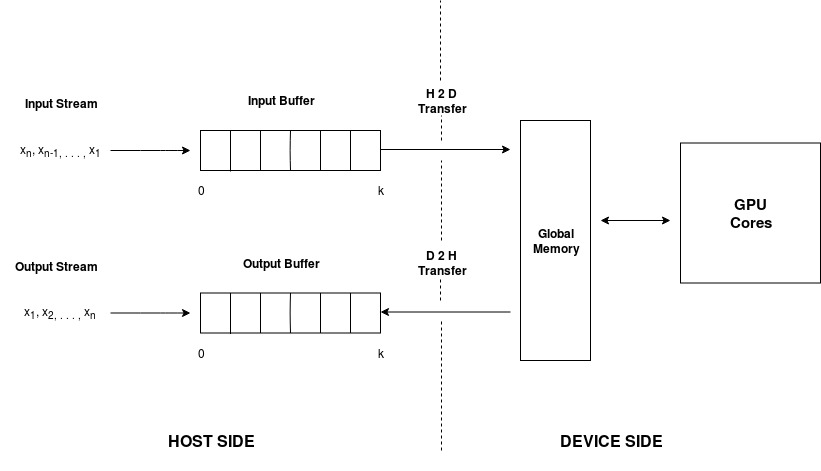
\includegraphics[width=\linewidth]{images/H2D.jpg}
		\caption{Here we have a general and broad graphical representation of our idea on how to fit a Farm parallel pattern on GPU architecture.}
		\label{fig:H2D}
	\end{figure}
	
	This behavior is illustrated graphically in Figure \ref{fig:H2D}. Here we can see our input stream and every \(k\) items we transfer them to Global memory of GPU.\\
	For reasons we showed in the previous sections, it would be unfeasible to work on single items but, at the same time, we should maintain a pattern as close as possible to Stream parallel. That's why we chose to work on chunks\footnote{We represented chunks as arrays, but they can be either small matrices or tiny images, as we'll see in \hyperref[chap:impl]{Chapter 4}.} of \(k\) items, where \(k\) is empirically determined to be a relatively small number of items and strictly related to execution configuration on kernel, in particular to block size.\\
	Items will be spread all over warps in a way such that for each item will be applied a set calculations, specified inside kernel code, that will be performed by one of the active threads in the warp.
	

	From that figure it may seems we're sending only \(k\) items at time to/from GPU, assuming \(k\) items in a buffer as a single item, this would correspond almost to a farm with one worker, processing one item per time. And this isn't completely what we wanted.\\
	\begin{figure}
		%	\hspace*{-2cm}  
		\vspace{-2cm}
		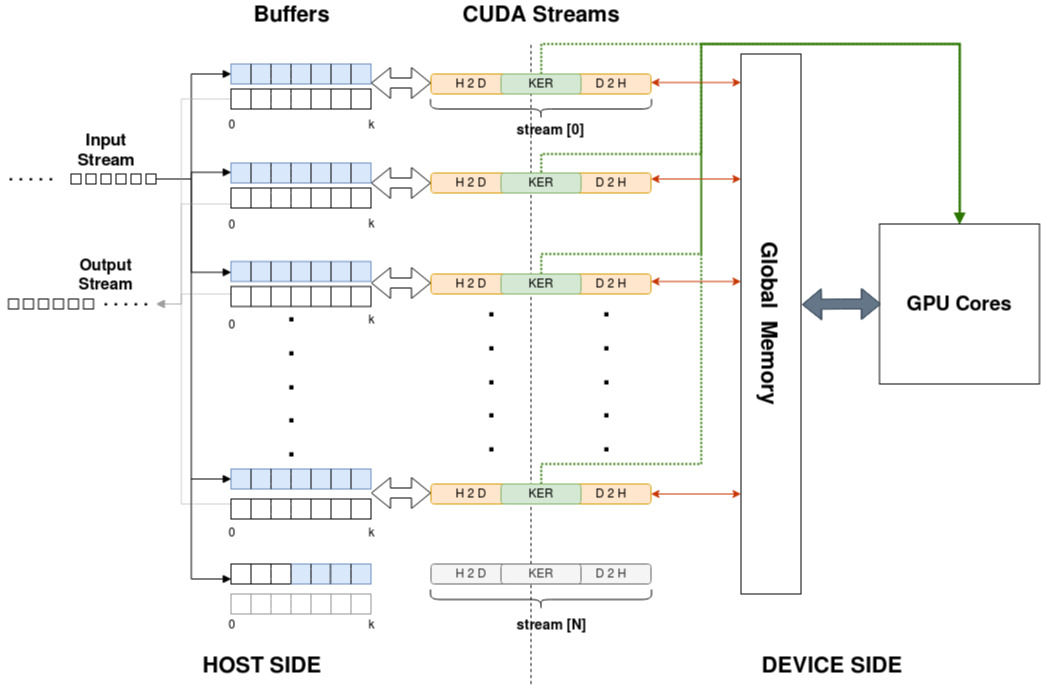
\includegraphics[scale=0.62,angle=-90]{images/overallLogic.jpg}
		\caption{Here we have a general and broad graphical representation of our idea on how to fit a Farm parallel pattern on GPU architecture.}
		\label{fig:overallLogic}
	\end{figure}
	So, here's where CUDA Streams \footnote{Don't confuse input/output stream in Farm parallel pattern with CUDA Streams.\\ These are two completely different notions: the first refers to the parallel pattern behavior of input/output data, the last refers to special CUDA commands (shown in \hyperref[subs:streams]{Section 2.3.3}).\\} come into play and we used them relying on the following ideas:
	\begin{enumerate}
		\item We have as many streams as Streaming Multiprocessors \footnote{Again CUDA Streams are a different concepts with respect to Streaming Multiprocessors. The first are a set of commands, the last are physical processing units.\\} and, at any given time, each of them hopefully issues a data transfer or a kernel executions;
		\item We should arrive at the point where each stream have issued at least one kernel launch, ideally we expect that each kernel execution is taken over by a certain multiprocessor. So we want to arrive at a moment in which we reach a work peak, where almost all SMs are busy;
		\item Obviously each kernel execution configuration should be well tuned, in order to take advantage of the maximum of resources in a multiprocessor. 
	\end{enumerate}
	

	All of those parameters have been established at first with some reasoning and assumptions on NVIDIA GPUs nature, later we moved on experimental proves \footnote{We'll see in next section more informations about Tunings.}. Measures and other estimation lead us to consider specific values for those variable parameters.\\
	So from the above facts is clear that we're trying to exploit each SM as a Farm parallel worker, furthermore, in such a way that all of those workers are as busy as possible. Note that our \textbf{SMs-workers} apply a \textbf{function-kernel} to all \textbf{tasks-chunks}.\\
	Bringing all pieces together we can summarize all project logic in Figure \ref{fig:overallLogic}.\\\\\\
	Putting down in words that schema:
				
		
	\begin{itemize}
		\item We have \(N\) CUDA streams, where \(N\) is the number of Streaming Multiprocessors in the machine were code is running;
		\item As input stream items arrive, we let them fill buffers;
		
		\item In a Round-Robin fashion we spread ready buffers all over the CUDA streams as follows:
		\begin{enumerate}
			\item As soon as the \(i^{th}\) buffer is full, it's asynchronously sent on \texttt{stream [i]} to the GPU, with the command \\ 
			\texttt{ \textbf{cudaMemcpyAsync}( devBuffer, hostBuffer, bytes, cudaMemcpyHostToDevice, \tab \tab \tab \tab stream [i]);}
			
			\item Soon after we put kernel call, on the \texttt{stream [i]}, to make desired computations on that buffer;
			
			\item Then, asynchronously again, we bring back results to host side, using the instruction \\
			\texttt{ cudaMemcpyAsync( devBuffer, hostBuffer, bytes, cudaMemcpyHostToDevice, \tab \tab \tab \tab stream[i]);}
			\item hopefully this should make a Streaming Multiprocessor,or a part, busy.
		\end{enumerate}
	\end{itemize}

	\begin{wrapfigure}[22]{r}{0.5\textwidth}
		%\begin{center}
		%\raggedleft
		\centering
		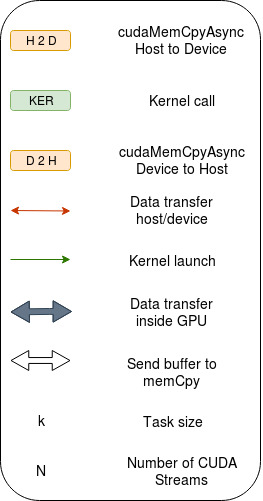
\includegraphics[width=1\linewidth]{images/logicLegenda.jpg}
		%\end{center}
		\caption{Legenda about Figure \ref{fig:overallLogic}.}
	\end{wrapfigure}
	Initially only few cores will be really busy, but as soon as the buffers and streams get full, the pressure on the GPU should increase, so we expected that workload should be enough to almost fill all of Streaming Multiprocessors.
	In particular, for us this means that we tried to have the maximum number possible of active threads inside each SM, having to do some work.\\
	Now let's put a magnifying glass upon Figure \ref{fig:overallLogic}, we want take a closer look to what we just said in Figure  \ref{fig:singleStream}.\\
	
	From that scheme, looking at violet numbered labels, we can see the order in which we issue commands in a stream, and this will be the order in which they will be issued to device side too, for that stream. \\
	The behavior of overlapping between different streams, isn't predictable. Anyway we should take advantage of the fact that, considering two different CUDA streams, we can overlap data transfer and/or kernel execution in a \texttt{stream [i]} with the ones in a \texttt{stream [k]} (for some \(k\in[0,N-1], \: for \: N =\# SMs\)). Obviously, when the number of streams is greater than 3, we can have only 2 data transfer operations issued at the same time (by two distinct streams) \footnote{As mentioned in \hyperref[chap:tools]{Chapter 2}, for concurrent memory copy between host and device, we have 2 copy engines.}.
	
	Note that in the Figure \ref{fig:singleStream}, we represented a single kernel execution as fully occupying an entire SM; in reality it's not exactly how it goes.
	We'll see how we practically tried out Streaming Multiprocessors \textit{occupancy} in  \hyperref[chap:experim]{Chapter 5}. \\
	
	So essentially if all of our reasoning and theories are right, we would expect that we can have an improvement, on completion time, roughly in the order of SMs number with respect to the \textit{classical approach}.\\
	By "classical approach" we mean to transfer data and execute kernels without any type of overlapping.\\ This is equivalent to send input to device, wait for data transfer completion on host, call kernel, send data back to host, only when all computations ended up, and finally results are transferred back to the host, waiting for data transfer ending.
	This similarly means that if, for example, we have 3 CUDA Stream we would expect to take an advantage on only at most 3 SMs (at peak work flow), so this should give us an improvement, in completion time, of at most 3 times compared to classical approach.\\

	\begin{figure}%[ht!]
		%	\hspace*{-2cm}  
		%\vspace{-2cm}
		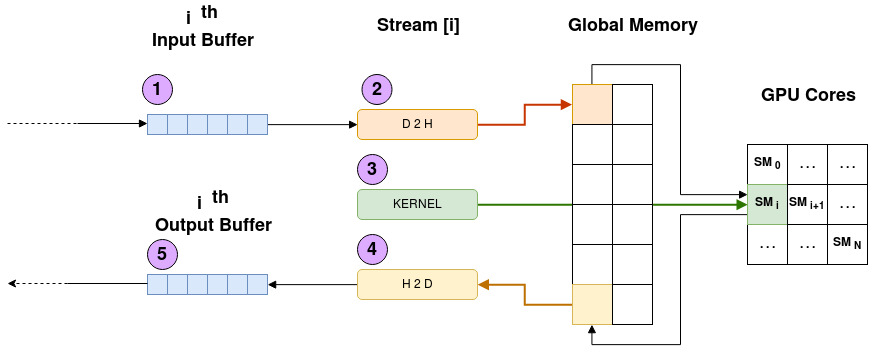
\includegraphics[scale=0.56]{images/singleStream.jpg}
		\caption{Here we can see what exactly happens in a certain CUDA Stream. Light violet numbered labels shows the order in which commands are issued by host to a certain stream.}
		\label{fig:singleStream}		
		
	\end{figure}	
\section{Tunings}
\label{sect:tunings}
	We showed a lot of peculiar behavior and architecture characteristics, because all of the above mentioned were taken into account for different implementation, tests datasets and results analysis.\\
	It's clear that, once we decided how to organize our Farm parallel pattern for the GPU, we had to give a huge work slice to experiments and empirical evaluations.
	This has many reasons why:
	\begin{itemize}
		\item It was important to think about a general logic, that wasn't architecture-dependent \footnote{At least we can say that the complexive view, showed in Fig. \ref{fig:overallLogic}, can be plausible with almost all NVIDIA architecture having >2 copy engines and allowing concurrent kernel execution. };
		
		\item To validate our total idea we had to make a lot of experiments, time measures, examples and even counterexamples;
		
		\item Clearly experiments required to get a little deeper on NVIDIA GPUs architecture, having a generic idea on good practices, not necessarily bounded to a specific model;
		
		\item Finally, we had to consider some feature totally model-bounded to launch tests and to give a sense to obtained results.
	\end{itemize}
	
	So after the logical phase, has followed a \textit{tuning phase}, that for first has been done facing general NVIDIA GPUs behavior and structure \footnote{In \hyperref[chap:experim]{Chapter 5} we'll mainly see tunings based on the GPUs used to run tests \textendash \textbf{P100} and \textbf{M40}.}.
	We followed for first some important best practices to try some good tunings:

	\begin{itemize}
		\item The effect of execution configuration on performance for a given kernel call generally
		depends on the kernel code, so experimentation is recommended and in fact we followed that approach;
		\item The number of threads per block should be chosen as a multiple of the warp size (generally equal to 32 threads) to avoid wasting computing resources with under-populated warps as much as possible \footnote{That's because kernels issue instructions in warps (groups of 32 threads). For example, if we have a block size of 50 threads, the GPU will still issue commands to 64 threads, so we would waste 14 of them idling.\\};
		\item We exploited \textbf{\textit{Occupancy Calculator}}\footnote{Those tools are included in CUDA Toolkit, they assist programmers in choosing thread block size based on kernel behavior, register and shared memory requirements.\\} both in spreadsheet and API functions\footnote{These are special function to call inside code, we'll see in \hyperref[chap:impl]{Chapter 4} a code example on how and where they are used.\\} formats , \cite{cudaguide}.
		 
	\end{itemize}

	Given those initial guidelines, it's important to highlight what are variable parameters in Figure \ref{fig:overallLogic}, on which the tuning was made:
	\begin{itemize}
		\item The number of Streams;		
		\item The number of blocks (grid size);
		\item The number of threads per block (block size) and as a consequence
		\item The buffer dimension.\\
	\end{itemize}
	After a lot of attempts and experiments, for each kernel type, we extrapolated best suitable values \footnote{Check \hyperref[chap:experim]{Chapter 5} to see all main values and their respective performances }.
 
			 
\subsection{Tuning on block and grid dimensions}
	It's important to understand some main concepts, that are the basis for the logic of this project.\\
	As we mentioned above, the variation on \textit{thread block size} and \textit{grid size}, can affect heavily performances, especially in an extreme scenario as the case study of this project.
	There's a tight bond in between \textit{Occupancy}, \textit{kernel execution configuration} and kernel code nature.
	For first note that a certain block, whatever its dimension is, will be run on a single Streaming Multiprocessor and once it's assigned it will never be moved; when resources are allocated for a thread block in an SM, it will become an \textit{active block}.\\
	In an SM we can have multiple blocks running independently, each of which grabbing its portion of resources, ie we can have multiple active blocks on a SM until they don't hit the maximum allowed.
	Here may emerge some particular cases:
	\begin{enumerate}
		\item Maximum block dimension (aka lot of threads per block), means that a smaller number of blocks, even only one, can fit in a certain SM;
		\item Small block dimension, means a higher number of blocks, even the maximum blocks number per SM supported, running on the same SM;
	\end{enumerate}
	
	In the first scenario, we can have cases of really good performances, but it may not be true when we have unbalanced workload for different blocks. This means that if a block has lot of work to do, it will monopolize resources of the SM in which it's running, making all other blocks, scheduled in the same SM, idle for too long (for example in our GPUs it may happens for \textit{blocksize = 1024}). 
	
	In the second scenario (for example for \textit{blocksize = 32}), we can have really poor performances due to poor resources exploitation, but for some kernels it may give a gain, especially in cases as the above mentioned of unbalanced workload.
	
	In general, there is a performance \textit{sweet spot} for middle values (for example usually identified in \textit{blocksize = 512}).\\
	%To better explain that concept, let's take a simple example. It's the first type of kernel we tested \footnote{We'll take a closer look on that case study, with implementation details, in \hyperref[chap:impl]{Chapter 4}.}, so suppose we have:
	%\begin{itemize}
	%	\item Vectors of floats as input and output;
	%	\item We have a "regular" kernel, in other words inside that we have not irregular workflows, we haven't divergent execution flowsand workload between all threads is almost the same;
	%	\item We avoid all types of synchronizations, both thread synchronization (\texttt{\_\_syncthreads()}) and host/device one (\texttt{cudaDeviceSynchronize()}).
	%\end{itemize}
	%In this situation
	So our tests had to face with the above explained behavior, without forgetting the nature of the various implemented kernels and the relative latencies.


\section{CPU/GPU Scheduling}
\label{sect:cpugpuscheduling}
In addition to the main logic of our project we introduced another branch of study.\\
In particular, we extended the Farm parallel pattern on GPGPU introducing a sort of \textit{\textbf{CPU/GPU Scheduler}}.\\
This consist in an implementation that, given an initial work percentage, it gradually and experimentally tunes those percentages to balance jobs.
In particular, the scheduler adjusts the dimensions of data chunks directed to CPU or GPU on the basis of previous measured completion times of both processors.\\
Clearly, starting from a user provided percentage, measured times are used to recompute percentages (and thus chunks dimension). So, in a finite number of algorithm steps, the two portion size will stabilize around two values.\\
This allow us to let host and device cooperate to apply same computations, but with different workloads. Clearly the main idea is to let GPU have a greater workload with respect to the one for CPU, so that  latter can be lighten from doing the entire computations; at the same time, having a good occupancy on GPU, we can gain a speedup compared to letting only one of the two processors doing all the work.\\

	

    \chapter{Implementation} 
\label{chap:impl}
Given the logical schema of the previous chapter, we had to build different types of code to observe their behaviors in performances.

In particular, we wanted to distinguish some kernels of interest and adapt them to the Farm parallel pattern for GPU we conceived. So, in this project we've implemented the following applications:
\begin{itemize}
	\item Repeated cosine application;
	\item Matrix multiplication;
	\item Blur Box filter.
\end{itemize}

\section{Kernels}
As we anticipated in the previous section, our kernels mainly doesn't use shared memory.\\
Each kernel clearly is designed such that each thread executes a different element from the input data structure.
\subsection{Repeated cosine}
	This is a very simple kernel, in which given as inputs an array of floating point and a number \textit{M}, it computes, for each input float, the cosine applied \textit{M} times. The output will be again a floats array (given by cosines).\\
	Note that, since here we're working on one-dimensional data structures, we'll use one-dimensional thread blocks for convenience.
	\begin{lstlisting}[language=C++]
	__global__ void cosKernel(int M, int N, float *x_d){  		  
		int idx = offset+blockIdx.x*blockDim.x + threadIdx.x; 		
		if(idx<N){		
			for(int j=0; j<M; ++j)
				x_d[idx]=cosf(x_d[idx]);  		
		}
		return ;
	}
	\end{lstlisting}
	This is almost a regular kernel, with no branching and an almost equal workload for each thread that could execute that code.\\
	It was a very useful kernel, because changing a single parameter we could then test situations either of low or high iterations amount, ie different workloads.
	Moreover this is clearly a computation-bounded kernel.
	
\subsection{Matrix multiplication}
	Here's the most classical version of matrix multiplication in CUDA.
    An important difference from the application above is that now we're working with matrices, both in input and output. So, for convenience, we'll use two-dimensional thread blocks.\\  
	Each couple of threads perform the computation of a single element in result matrix. For example, assume we have \texttt{thread[ROW]} and \texttt{thread[COL]}, then they will perform\\ \texttt{sum += A[ROW, i] * B[i, COL];},\\ where \texttt{i = 0, ..., N} and \texttt{sum} will be \texttt{C[ROW, COL]}, ie one of the items result matrix.
	\begin{lstlisting}
	/**** MATMUL ****/
	__global__ void matMulKernel(float* A, float* B, float* C, int m, int k, int n) {   
		int ROW = blockIdx.x*blockDim.x+threadIdx.x;
		int COL = blockIdx.y*blockDim.y+threadIdx.y;
		
		if (ROW<m && COL<n) {
			float tmpSum = 0.0f;			
	
			for (int i = 0; i < k; ++i) {
				tmpSum += A[(ROW*k)+i] * B[(i*n)+COL];
			}        
			C[(ROW*n)+COL] = tmpSum;
		}
		return ;
	}
	
		
	/**** SQUARE MATMUL ****/
	__global__ void squareMatMulKernel(float* A, float* B, float* C, int N) {

		int COL = blockIdx.x*blockDim.x+threadIdx.x;
		int ROW = blockIdx.y*blockDim.y+threadIdx.y;
		
		if (ROW<N && COL<N) {
			float tmpSum=0.0f;        
		
			for (int i = 0; i < N; ++i) {
				tmpSum += A[(ROW*N)+i] * B[(i*N)+COL];
			}        
			C[(ROW*N)+COL] = tmpSum;        
		}
		return ;
	}
	\end{lstlisting}
	Matrix multiplication is one of the most widespread applications in GPU computing, this is the basis of other applications too.\\
	It is well known that this kind of very trivial matrix multiplication is quite inefficient. In fact, each for loop iteration will have to perform a multiplication and a sum but, at the same time, the GPU will have to access global memory three times \footnote{We'll have two pull from memory for A[i, k] and B[k, j] and a push for C[i, j].}.
	This means we have a low arithmetic intensity w.r.t. memory accesses, so cores won't hide memory access latency.
	That's why in general other optimized algorithms are used, the most known of them is the one decomposing matrices in tiles that will fit in \textit{shared memory}.
	
\subsection{Blur Box filter}
	The last type of application implemented in this project is an image processing kernel to apply blur filter.
	Here input and output pictures are represented as char buffer, items are \textbf{RGB} values in [0, 255] that represent pixels such as "RGB RGB RGB...".\\
	For each pixel, in the input image, we take the average of each of the pixels in neighborhood (inside the limits of filter size) and writes it to the output image. This filter is known as a Box blur \footnote{Another blur filter is the \textit{Gaussian blur}, generally preferred as to be more accurate. In fact Box blurs are frequently used to approximate a Gaussian blur. By the central limit theorem, repeated application of a box blur will approximate a Gaussian blur.}.
	
%	Notice that we check if our offset is actually within the range of \texttt{width*height}, because it can happen that it will be outside due to the blocks CUDA will run, so remember to keep that. Also we need to remember to check whether or not the pixel we read are actually in our image when doing the box blur as well. You can try to remove them one at a time and see what happens.
	\begin{lstlisting}
	/**** BLURBOX ****/
	__global__ void blurBoxFilterKer(unsigned char* input_image, unsigned char* output_image, int width, int height) {
	
		const unsigned int offset = blockIdx.x*blockDim.x+threadIdx.x;
		int dim = width*height*3;
		if(offset<dim){
			int x = offset % width;
			int y = (offset-x)/width;
			int fsize = 5; // Filter size
			if(offset < width*height) {
				float output_red = 0;
				float output_green = 0;
				float output_blue = 0;
				int hits = 0;
				for(int ox = -fsize; ox < fsize+1; ++ox) {
					for(int oy = -fsize; oy < fsize+1; ++oy) {
						if((x+ox) > -1 && (x+ox) < width && (y+oy) > -1 && (y+oy) < height) {
							const int currentoffset = (offset+ox+oy*width)*3;
							output_red += input_image[currentoffset]; 
							output_green += input_image[currentoffset+1];
							output_blue += input_image[currentoffset+2];
							hits++;
						}
					}
				}
				output_image[offset*3] = output_red/hits;
				output_image[offset*3+1] = output_green/hits;
				output_image[offset*3+2] = output_blue/hits;
			}
		}
		return;
	}
	\end{lstlisting}

\section{Parallel Patterns implementation on GPU}
What really makes the difference in the implementation is how we send data to the GPU and kernel executions configurations.
This is what really determines a behavior associated to either a Stream Parallel pattern or a Data Parallel pattern.


\subsection{Stream Parallel on GPU}
	The code translates the diagram in Fig. \ref{fig:overallLogic}.
	Let's start by explaining the setting phase:
	\begin{itemize}
		\item The block dimension is provided as command line parameter;
		\item Then grid dimensions are initially determined;
		\item Here we can have two different settings
		\begin{itemize}
			\item The chunk has the same dimension of the block, given the capabilities in our machines means having a size \(< 1024\). The grid will have size one;
			\item The chunk takes as dimension the maximum number of threads active in a SM, for both our machines is 2048. Here the grid will be adjusted to cover the chunk dimension w.r.t. the block dimension, ie \texttt{GRID = maxThreads/BLOCK;}
		\end{itemize}
	
	\end{itemize}
		\begin{lstlisting}		
		#ifdef LOWPAR
			GRID = 1;
			chunkSize = BLOCK*GRID;		
		#else
			GRID = maxThreads/BLOCK;  
			chunkSize = BLOCK*GRID;		
		#endif		
		\end{lstlisting}
	
	Now we arrive at the core of the implementation. The number of CUDA streams to spawn, as we previously told, is equal to the number of Streaming multiprocessor in the target machine. So, we start by distinguish two different cases:
	\begin{itemize}
		\item Number of streams equal to zero, this means we won't use CUDA stream
		\begin{enumerate}
			\item We allocate space for our device chunk, with a simple \texttt{cudaMalloc} (because here we'll not use streams);
			\item As input stream items arrive, we store them on the host chunk buffer;
			\item We send it to the device as soon as it's full, with a simple \texttt{cudaMemcpy} \footnote{Note that \texttt{cudaMemcpy} is a blocking operation w.r.t. the host, this means that other CUDA calls from the host will be issued after data is fully copied to device.};
			\item We launch the Kernel, that will execute as soon as data is fully copied;
			\item We call another \texttt{cudaMemcpy} to bring back results to host.
		\end{enumerate}
		
			\begin{lstlisting}[label=lst:noStr]
			void cosKer(int m, int chunk, float *x, float *cosx, float *x_d)
			{   
				int xBytes = chunk*sizeof(float);
				
				gpuErrchk( cudaMemcpy(x_d, x, xBytes, cudaMemcpyHostToDevice) ); 
				
				cosKernel<<<GRID, BLOCK>>>(m, chunk, x_d);
				#ifndef MEASURES
					gpuErrchk( cudaPeekAtLastError() );
					gpuErrchk( cudaDeviceSynchronize() );
				#endif   
				
				gpuErrchk( cudaMemcpy( cosx, x_d, xBytes, cudaMemcpyDeviceToHost) );
			}
			\end{lstlisting}
		
		\item Number of streams greater than zero, this means we will use CUDA stream, so steps are analogous to the previous except for some tricks (See Code Listing )
		\begin{enumerate}
			\item We allocate space for our device chunk, with a \texttt{cudaMallocHost} (in order to use CUDA streams and gain best overlapping possible, host should allocate memory as \textit{Pinned});
			\item In a Round-Robin fashion, we send full chunks in an asynchronous way, using \texttt{cudaMemcpyAsync} \footnote{Note that \texttt{cudaMemcpyAsync} is non-blocking for the host, in parameters we'll have to specify which stream will issue the copy.};
			\item We launch the Kernel in the same CUDA stream of the previous copy;
			\item We call another \texttt{cudaMemcpyAsync} to bring back results to host, on the same stream as before.
		\end{enumerate}
		
		\begin{lstlisting}[label=lst:str]
		void cosKerStream(int m, int chunk, float *x, float *cosx, float *x_d, cudaStream_t strm, int strBytes)
		{     
			gpuErrchk( cudaMemcpyAsync(x_d, x, strBytes, cudaMemcpyHostToDevice, strm) ); 
			
			cosKernel<<<GRID, BLOCK, 0, strm>>>(m, chunk, x_d);
			
			#ifndef MEASURES
				gpuErrchk( cudaPeekAtLastError() );
				gpuErrchk( cudaDeviceSynchronize() );
			#endif   
			gpuErrchk( cudaMemcpyAsync( cosx, x_d, strBytes, cudaMemcpyDeviceToHost, strm) );
		}
		\end{lstlisting}
		
	\end{itemize}
	The reason why we implemented these two versions, of Farm Parallel Pattern for GPU, is that we want to show the gain obtained with CUDA Stream.\\
	In particular we want to show that a Stream Parallel Pattern would be unfeasible in terms of device completion time, because of overhead introduced by data transfers. Instead, we wanted to show that, with CUDA Streams and some other precautions and experiments, a Stream Parallel Pattern could work near to the Data Parallel performances.\\
	
	It may be interesting to see how the Round Robin scheduler sends buffers to the function \texttt{cosKerStream} via CUDA streams, we present a pseudo-code version that shows only main features:
	\begin{lstlisting}
	const int streamBytes = chunkSize*sizeof(float) ;
	int strSize = nStreams*chunkSize;	
	//host pinned mem
	gpuErrchk( cudaMallocHost((void **)&x, strSize*sizeof(float)) ); 
	gpuErrchk( cudaMallocHost((void **)&cosx, strSize*sizeof(float)) ); //pinned cosx
	//device memory	
	gpuErrchk( cudaMalloc((void**)&x_d, strSize*sizeof(float)) );
	//stream array and events creation 
	cudaStream_t streams[nStreams];
	streamCreate(streams, nStreams);
	createAndStartEvent(&startEvent, &stopEvent);
	
	int k=0;
	while (InputStream) {  
		if (buffer x[i: i+chunkSize] is full)
		{
			int i = k%nStreams;
			int strOffs = i*chunkSize;
			
			cosKerStream( M_iterations, chunkSize, x[i: i+chunkSize], cosx[i: i+chunkSize], x_d[i: i+chunkSize], streams[i], streamBytes);     
			   
			send output buffer cosx[i: i+chunkSize] to output stream
			
			++k;
		}
		else
		{
			add item to buffer x[i: i+chunkSize]
		}	
	} 
	msTot = endEvent(&startEvent, &stopEvent);
	streamDestroy(streams,nStreams); 	
	\end{lstlisting}
	It's interesting to highlight the use of \textit{CUDA Events}, they were useful to measure the completion time of memory copies and kernel executions. So they allowed us to make device side measures, that are the main concern in this project \footnote{We'll explain other details on measures on \hyperref[chap:experim]{Chapter 5}.}.
	
	As we can see we presented most important code parts relative to the Cosine Kernel, but the structure and the implementation to execute Matrix multiplication and Blur Box are totally analogous.

\subsection{Data Parallel un GPU}
	To prove that our Farm Pattern had acceptable performances, it was useful to compare it with its respective Data Parallel version.\\
	Clearly, to have control on time probes and to compare such two different models, we set a maximum length on input stream. In the reality we know that we cannot have such informations on input/output streams. So we make the assumptions to know input stream length only for a time measuring purpose.
	
	Furthermore, this allow us to compare our Farm model, having an input stream of \texttt{N\_size} items length, with a Data Parallel model sending all \texttt{N\_size} items in once, computing them all in a classic configuration kernel and send back all again \footnote{And this is how generally the GPU is meant to be used and this is the kind of problem a GPU is designed for.}
	\begin{lstlisting}
	x = (float *) malloc(N_size*sizeof(float));
	cosx = (float *) malloc(N_size*sizeof(float));
	gpuErrchk( cudaMalloc((void**)&x_d, N_size*sizeof(float)) );
	
	generate N_size items and put in the "x" data structure
	
	createAndStartEvent(&startEvent, &stopEvent);
	
	float msKer = optimalCosKer(M_iter, N_size, x, cosx, x_d, clocks, clocks_d); 	
	
	
	/*** Kernel launcher ***/
	float optimalCosKer( int m, int n, float *x, float *cosx, float *x_d){
		int gridSize;    // The actual grid size needed, based on input size 
		int minGridSize; // The min grid size needed to achieve the maximum occupancy for a full device launch 
		cudaEvent_t startEvent, stopEvent;
		
		cudaOccupancyMaxPotentialBlockSize( &minGridSize, &BLOCK, cosKernel, 0, 0); 
		GRID = (n + BLOCK - 1) / BLOCK; // Round up according to array size 

		gpuErrchk( cudaMalloc((void**)&clocks_d, GRID*sizeof(int)) );  		
		createAndStartEvent(&startEvent, &stopEvent); 
		  
		gpuErrchk( cudaMemcpy(x_d, x, n*sizeof(float), cudaMemcpyHostToDevice) ); 
		
		cosKernel<<<gridSize, blockSize>>>(m, n, x_d);
		
		gpuErrchk( cudaMemcpy( cosx, x_d, n*sizeof(float), cudaMemcpyDeviceToHost) );
	
		gpuErrchk( cudaPeekAtLastError() );		
		cudaDeviceSynchronize();		
		float ms = endEvent(&startEvent, &stopEvent);
	
		return ms;	
	}
		
	\end{lstlisting}
	The peculiarity of this Kernel is that we exploited CUDA Occupancy APIs.
	The occupancy-based launch configurator APIs,
	\texttt{cudaOccupancyMaxPotentialBlockSize}, heuristically calculate an execution configuration (thread block and grid sizes) that achieves the maximum multiprocessor-level occupancy.\\
	This was one example of the use of CUDA Occupancy calculator tools, in this case we used it to achieve the best block and grid configuration possible for our Kernel.
	
	Again the code presented above is relative to Cosine kernel, but the implementation structure is analogous to the one for Matrix multiplication and Blur Box.
	For example, in Matrix multiplication, we'll have a stream of small matrices for Farm parallel and a single huge matrix for Data parallel.
	
	
	
\section{CPU and GPU Mix}
%Queue with P and Q chunk exec by respectively CPU and GPU.

    \chapter{Experiments}
\label{chap:experim}
%\section{Overview}
In this chapter will be shown all the experiments performed and their results. The first section starts from what we expect to show from experiments on code and, to this aim, what kind of comparisons will be made.\\
The second section will explain how to implement tests, ie chosen datasets for each type of code and scripts main features.
After that, the other section will move on results, in particular will be shown time measures and plots with some final remarks and comparisons with respect to what we expected.

%\section{What and How}
%What and How
\section{Expectations}
As previously mentioned, what we want to see is that our model and implementation of a Farm parallel pattern can fit in a GPU.
To this aim is necessary to gain a speedup in the order of the number of Streaming multiprocessors of the GPU we're running code.
Let's clarify some concepts in the sentence above:

\begin{itemize}
	\item The speedup will be estimated in terms of \textbf{GPU completion time}, ie the total time needed to perform all data transfers and kernel executions for a certain application;
	\item We expect to have the best speedup only when we have certain conditions;
	\item The best speedup for would be in the order of multiprocessors number.
\end{itemize}
The last point means we can't expect to reach greater gain than the available amount of hardware resources. This is strictly related to the fact that we can't expect Streaming parallel problems, that we implemented, to perform better than the equivalent Data Parallel version. \footnote{As we mentioned in previous Chapters, the GPU is specifically designed to be efficient and to perform at its best on Data Parallel problems.}
The second point above means we expect the best performances in the following cases:
\begin{itemize}
	\item When we have a regular kernel, that is a kernel with the lowest possible amount of branching and, thus, very low (or absent) threads divergence;
	\item When the kernel is more computational-bound than memory bound, the less access to Global memory the less data transfer latency will slow down computations;
	\item When the kernel execution takes an amount of time near the one for a data transfer.
\end{itemize} 
When one, or more, of the above conditions isn't meet we expect to have a considerably lower speedup.


\subsection{Measures: What and How}
Before the test setup and writing it's important to understand what we should measure, in order to get significant comparisons.\\
First we recall that the measures of interest are relative to \textit{data transfers} and \textit{kernel execution}. Clearly, in the case were CUDA streams are used, we have an additional time cost to create and destroy streams, especially when lot of streams are spawned.\\
For completeness some measures on CUDA Stream creation/destruction \footnote{Measures on CUDA Streams spawn/deletion are collected from \textit{nvprof} log file, where all CUDA APIs time is precisely measured.} will be reported, but we won't sum up them with measures on data transfer and kernel execution. This is because, even if the streams overhead can be notable \footnote{We'll see that CUDA streams creation/destruction can take from few to hundred milliseconds, depending on how many they are.}, it's a one-time cost to pay.\\
This means that it won't weigh on performances, given that in the beginning we create CUDA streams, then we'll run kernels on a indefinitely long input stream and, only when input is totally consumed out, CUDA streams will be destroyed. 
So on a reasonably long input stream, the CUDA streams APIs cost should be negligible.

So focusing on data transfers and kernel, we put two time probes, one before the start of the input stream loop and one at the end. The time probes are implemented using \textbf{CUDA Events}.\\
Below will be reported a pseudo-code to clarify how the probes are positioned:
\begin{lstlisting}[label={lst:timers}]	
/**** Code with events time probes ****/	
streamCreate(streams, nStreams); // Create CUDA streams

createAndStartEvent(&startEvent, &stopEvent); // Create "start" and "stop" events, start recording

int k = 0;
while (InputStream) {  
	if (buffer x[i: i+chunkSize] is full)
	{
		int i = k%nStreams;
		
		kernelCaller(input_host, output_host, input_device, output_device, streams[i], streamBytes, ...);

		. . . .
		
		++k;
	}
	else
	{
		add item to buffer x[i: i+chunkSize]
	}	
} 
msTot = endEvent(&startEvent, &stopEvent);
cudaEventDestroy();
		
/**** Events Creation and start ****/
void createAndStartEvent(cudaEvent_t *startEvent, cudaEvent_t *stopEvent)
{
	gpuErrchk( cudaEventCreate(startEvent) );
	gpuErrchk( cudaEventCreate(stopEvent) );
	gpuErrchk( cudaEventRecord(*startEvent,0) );
}

/**** Events end and time measure collection ****/
float endEvent(cudaEvent_t *startEvent, cudaEvent_t *stopEvent)
{
	float ms = 0.0f;
	gpuErrchk( cudaEventRecord(*stopEvent, 0) );
	gpuErrchk( cudaEventSynchronize(*stopEvent) );
	gpuErrchk( cudaEventElapsedTime(&ms, *startEvent, *stopEvent) );
	return ms;
}
	
/**** Kernel caller example ****/
void kernelCaller(input_host, output_host, input_device, output_device, streams[i], streamBytes, ...)
{
	// H2D mem copy 
	gpuErrchk( cudaMemcpyAsync(input_device, input_host, streamBytes, cudaMemcpyHostToDevice, streams[i]) ); 
	// Kernel call
	ernel<<<GRID, BLOCK, 0, streams[i]>>>(input_device, output_device, ...); 
	#ifndef MEASURES
	gpuErrchk( cudaPeekAtLastError() );
	#endif   
	// D2H mem copy 
	gpuErrchk( cudaMemcpyAsync( output_host, output_device, streamBytes, cudaMemcpyDeviceToHost, streams[i]) );
}
	
\end{lstlisting}
CUDA event APIs are a device-bound tool and they were chosen as inside-code measurement for several reasons.
Another approach could be to use any CPU timer provided for C++ in a way such as:
\begin{lstlisting}
	t1 = myCPUTimer();
	Kernel<<<GRID, BLOCK>>>(param0. param1, ...);
	cudaDeviceSynchronize();
	t2 = myCPUTimer();
\end{lstlisting}
A problem with using host-device synchronization points, such as \texttt{cudaDeviceSynchronize()}, is that they stall the GPU pipeline.
Events, instead, provide a relatively light-weight alternative to CPU timers via the \textit{CUDA event API}. This API includes calls to create and destroy events, record events, and compute the elapsed time in milliseconds between two recorded events, exactly as it's shown in code Listing \ref{lst:timers}.

CUDA events make use of the concept of CUDA streams. 
CUDA events are of type \texttt{cudaEvent\_t} and are created and destroyed with \texttt{cudaEventCreate()} and \texttt{cudaEventDestroy()}. In the above code \texttt{cudaEventRecord()} places the start and stop events into the default stream, or \texttt{stream 0} (also called the “\textit{Null Stream}”). This holds for all device timers we introduced in our code.\\
The \texttt{cudaEventRecord()} will record a time stamp in device for the event, but only when that event is reached in the specified stream. The function \texttt{cudaEventSynchronize()} blocks CPU execution until the specified event is recorded. The \texttt{cudaEventElapsedTime()} function returns in the first argument the number of milliseconds time elapsed between the recording of \textit{start} and \textit{stop}. This value has a resolution of approximately 0.5 microseconds \cite{devblogevents}. So those timers will be enough accurate for our purpose, since we'll see that almost all elapsed times will be from tens to hundreds milliseconds.

It's important to point out why we used events on the default stream. 
If one of the events were last recorded in a non-NULL stream, the resulting time may be greater than expected (even if both used the same stream handle). This happens because the \texttt{cudaEventRecord()} operation takes place asynchronously and there is no guarantee that the measured latency is actually just between the two events.\\
Any number of other different stream operations could execute in between the two measured events, thus altering the timing in a significant way \cite{libevents}.
So given the asynchronous nature of CUDA calls we do in non-default stream, the behavior and order in between different streams is unpredictable. This means that a call from a different non-null stream can actually be issued in between two events we're trying to recording, even if they were issued from the same non-default stream.

Another significant fact on events, is why we chose to put timers outside the loop over input stream.
We could insert events again on default stream, but inside the loop, so that we measured singularly each iteration\footnote{And so measure each single memory copy H2D, Kernel execution and memory copy D2H.} and sum up all those elapsed times.
There would have been three problems:
\begin{itemize}
	\item Each "\textit{end}" event, must be sure to measure everything until the ending event, that's why it's necessary to introduce \texttt{cudaEventSynchronize()};
	\item Given that the input stream should be quite long, all those timers in each loop iteration would have introduced an amount of undesired overhead, apart from synchronization time.
\end{itemize}

In first problem we recall that \texttt{cudaEventSynchronize()} blocks CPU execution until the specified event is recorded,but we really want to avoid that.
We should avoid as much host-device synchronizations as we can: given that we're working on input/output streams of items from host and, thus, "stopping" this flow on host side at each iteration would invalidate the gain of our model, increasing the overall completion time (of a non negligible amount).\\
The second problem is related to the first. Even if events are a light-weight solution for device activities timing, it doesn't mean they don't introduce a bit of overhead (in addition to the synchronization one) in both host and device side.

For completeness, we'll show some performances case of interest measured by profilers, in addition to those from timers.
This will allow us not only to observe the correctness of some measurements, but also to check some special cases or technical details.


\subsection{Tests setup}
Once it is determined the time measure criterion, we have to decide what behaviors we want to observe from our code and its performances.
Note that for each type of input dataset, we run multiple times (say \(N_{test}\)) the executable so that, for a certain input setup, we can collect more time measures. This allows us to delete some \textit{outliers} completion times, as they may distort the result, and then we take the mean value among the remaining measures.

Moreover, as we mentioned in \hyperref[subs:bash]{Subsection 2.5.1}, we implemented our tests as bash scripts.
These scripts will cover the task of:
\begin{itemize}
	\item Compiling a certain executable, exploiting the rules available in our Makefile;
	\item Run that executable \(N_{test} - 1\) times and then redirect the output, of the running application, to a specific \texttt{.txt} file;
	\item Run for the \(N_{test}^{\ th}\) time the executable via \texttt{nvprof}, redirecting the profiler output to a folder of \texttt{.txt} log files
\end{itemize} 
In next sections we'll show, for each type of kernel, what type of tests have been made and relative results.

It's important to recall that input stream length shouldn't be known a priori, but in tests we'll see that we have to give an input a limit. This is for time measuring purpose only, because we need to have a knowledge on what and how much data we are measuring.


\subsection{Speedup}
\label{susb:speedup}
Two important metrics related to performance and parallelism are \textbf{speedup} and \textbf{efficiency}. Speedup compares the latency for solving a certain computational problem on one hardware unit, generally referred to as \textit{worker}, versus solving the same problem on P hardware units, as below
\begin{center}
	\(speedup = S_{P} = \frac{T_{1}}{T_{P}} \)
\end{center}


where \(T_{1}\) is the latency of the program with one worker and \(T_{P}\) is the latency on P workers.
\textbf{Efficiency} is speedup divided by the number of workers:
\begin{center}
\(efficiency = \frac{S_{P}}{P} =  \frac{T_{1}}{P \cdot T_{P}}\)
\end{center}
Efficiency measures return on hardware investment. Ideal efficiency is 1 (often reported as 100\%), which corresponds to a linear speedup, but many factors can reduce efficiency below the ideal.
If T 1 is the latency of the parallel program running with a single worker, Equation 2.1 is sometimes
called relative speedup, because it shows relative improvement from using P workers. This uses a
serialization of the parallel algorithm as the baseline. However, sometimes there is a better serial algo-
rithm that does not parallelize well. If so, it is fairer to use that algorithm for T 1 , and report absolute
speedup, as long as both algorithms are solving an identical computational problem. Otherwise, using
an unnecessarily poor baseline artificially inflates speedup and efficiency.
In some cases, it is also fair to use algorithms that produce numerically different answers, as long
as they solve the same problem according to the problem definition.\\ 
An algorithm that runs P times faster on P processors is said to exhibit \textbf{linear speedup}. It is rare in practice, since there is extra work, involved in distributing work to processors and coordinating them. This extra work clearly introduces extra time, also known as \textbf{overhead}.\\
In addition, an optimal serial algorithm may be able to do less work overall than an optimal parallel algorithm for certain problems, so the achievable speedup may be sublinear in P, even
on theoretical ideal machines. Linear speedup is usually considered optimal since we can serialize the parallel algorithm, as noted above, and run it on a serial machine with a linear slowdown as a worst-case baseline.\\
However, as exceptions, an occasional program will exhibit \textbf{superlinear speedup} \footnote{Some common causes of superlinear speedup include:
	
	- Restructuring a program for parallel execution can cause it to use cache memory better, even when
	run on with a single worker! But if T 1 from the old program is still used for the speedup calculation,
	the speedup can appear to be superlinear. See Section 10.5 for an example of restructuring that often
	reduces T 1 significantly.
	- The program’s performance is strongly dependent on having a sufficient amount of cache memory,
	and no single worker has access to that amount. If multiple workers bring that amount to bear,
	because they do not all share the same cache, absolute speedup really can be superlinear.
	- The parallel algorithm may be more efficient than the equivalent serial algorithm, since it may be
	able to avoid work that its serialization would be forced to do. For example, in search tree problems,
	searching multiple branches in parallel sometimes permits chopping off branches (by using results
	computed in sibling branches) sooner than would occur in the serial code.} — an efficiency greater than 100\%. 

However, in general, sublinear speedup is the norm.
Section 2.5.4 discusses an important limit on speedup: Amdahl’s Law. It considers speedup as P varies and the problem size remains fixed. This is sometimes called strong scalability. Section 2.5.5 discusses an alternative, Gustafson-Barsis’ Law, which assumes the problem size grows with P.
This is sometimes called weak scalability. But before discussing speedup further, we discuss another
motivation for parallelism: power \cite{structparprog}.


%. . . the effort expended on achieving high parallel processing rates is wasted unless it is accompanied by achievements in sequential processing rates of very nearly the same magnitude.

Amdahl argued that the execution time \(T_{1}\) of a program falls into two categories:

- Time spent doing non-parallelizable serial work
- Time spent doing parallelizable work
Call these \(T_{ser}\) and \(T_{par}\) , respectively. \\
Given P workers available to do the parallelizable work, the times for sequential execution and parallel execution are:
\begin{center}
	\(T_{1} = T_{ser} + T_{par}\) \\
	\(T_{P} \geq T_{ser} + \frac{T_{par}}{P}\)
\end{center}

The bound on \(T_{P}\) assumes no superlinear speedup, and is an exact equality only if the parallelizable work can be perfectly parallelized.

Plugging these relations into the definition of speedup yields \textbf{Amdahl’s Law}:
\begin{center}
	\(S_{P} \leq \frac{T_{ser}+T_{par}}{T_{ser}+T_{par}/P}\)
\end{center}
Amdahl’s Law has an important corollary. Let \(f\) be the non-parallelizable serial fraction of the total work. Then the following equalities hold:
\begin{center}
	\(T_{ser} = f \cdot T_{1}\)\\
	 \(T_{par} = (1-f) \cdot T_{1}\)
\end{center}

Substituting these into Equation **** and simplify to get:
\begin{center}
	\(S_{P} \leq \frac{1}{f+(1-f)/P}\)
\end{center}
And so when P tends to infinity
\begin{center}
	\(S_{\infty} \leq \frac{1}{f}\)
\end{center}

Speedup is limited by the fraction of the work that is not parallelizable, even using an infinite number
of processors.\\
For example if 10\% of the application cannot be parallelized, then the maximum speedup is 10x.
If 1\% of the application cannot be parallelized, then the maximum speedup is 100x.\\
In practice, an infinite number of processors is not available. With fewer processors, the speedup may be reduced, so the equation above gives an upper bound on the speedup.

%This limitation on speedup can also be viewed as inefficient use of parallel hardware resources for large serial fractions, as shown in Figure 2.6.

Amdahl's Law views programs as fixed and the computer as changeable, but experience indicates
that as computers get new capabilities, applications change to exploit these features.\\
% Most of today's applications would not run on computers from 10 years ago, and many would run poorly on machines that are just 5 years old.
%More than two decades after the appearance of Amdahl’s Law, John Gustafson noted that several programs at Sandia National Labs were speeding up by over 1000×. Clearly, Amdahl’s Law could be evaded.
Gustafson noted that problem sizes grow as computers become more powerful. As the problem
size grows, the work required for the parallel part of the problem frequently grows much faster than
the serial part.\\
If this is true for a given application, then as the problem size grows the serial fraction decreases and speedup improves.
Suppose that the serial portion is constant while the parallel portion grows linearly with the problem size. As workers are added, the application solves bigger problems in the same time, or the same problem in less time.\\
The serial portion still takes the same amount of time to perform, but diminishes as a fraction of the whole. Once the serial portion becomes insignificant, speedup grows practically at the same rate as the number of processors, thus achieving linear speedup.

Both Amdahl’s and Gustafson-Barsis’ Laws are correct. The difference lies in whether we want to make a program run faster with the same
workload or run in the same time with a larger workload.\\
%History clearly favors programs getting more complex and solving larger problems, so Gustafson’s observations fit the historical trend. Nevertheless, Amdahl’s Law still haunts you when you need to make an application run faster on the same workload to meet some latency target.
Furthermore, Gustafson-Barsis’ observation is not a license for carelessness. In order for it to
hold it is critical to ensure that serial work grows much more slowly than parallel work, and that
synchronization and other forms of overhead are scalable.


2.5.6 Work-Span Model
This section introduces the work-span model for parallel computation. The work-span model is much
more useful than Amdahl’s law for estimating program running times, because it takes into account
imperfect parallelization. \\
Furthermore, it is not just an upper bound as it also provides a lower bound.
It allows to estimate \(T_{P}\) from just two numbers: \(T_{1}\) and \(T_{\infty}\).

In the work-span model, tasks form a directed acyclic graph. A task is ready to run if all of its predecessors in the graph are done. 
The basic work-span model ignores communication and memory access costs. It also assumes task scheduling is greedy, which means the scheduler never lets a hardware worker sit idle while there is a task ready to run.

The extreme times for\(P=1\) and \(P=\infty\) are most important.\\
Time \(T_{1}\) is called the \textbf{work} of an algorithm. It is the time that a serialization of the algorithm would take and is simply the total time it would take to complete all tasks.\\
Time \(T_{\infty}\) is called the \textbf{span} of an algorithm. The span is the time a parallel algorithm would take on an ideal machine with an infinite number of processors.

%Span is equivalent to the length of the critical path. The critical path is the longest chain of tasks that must be executed one after each other. 
%Figure 2.8 shows an example. Each box represents a task taking unit time, with arrows showing dependencies. The work is 18, because there are 18 tasks. The span is 6, because the longest chain of tasks that must be evaluated one after the other contains 6 tasks.
Work and span each put a limit on speedup.\\ Superlinear speedup is impossible in the work-span
model:
\begin{center}
	\(S_{P} = \frac{T_{1}}{T_{P}} \leq \frac{T_{1}}{T_{1}/P} = P\)
\end{center}
On an ideal machine with greedy scheduling, adding processors never slows down an algorithm:
\begin{center}
	\(S_{P} = \frac{T_{1}}{T_{P}} \leq \frac{T_{1}}{T_{\infty}}\)
\end{center}
In words:
\begin{center}
	\(speedup = \frac{work}{span}\)
\end{center}
Real machines introduce synchronization overhead, not only for the synchronization constructs themselves, but also for communication. A span that includes these overheads is called a \textbf{burdened span}.

The span can also be used to estimate a lower bound on speedup for an ideal machine. An inequality known as Brent's Lemma bounds \(T_{P}\) in terms of the work \(T_{1}\) and the span \(T_{\infty}\):
\begin{center}
	\(T_{P} = \frac{T_{1}-T_{\infty}}{P+T_{\infty}}\)
\end{center}
Here is the argument behind the lemma. The total work \(T_{1}\) can be divided into two categories:
perfectly parallelizable work and imperfectly parallelizable work. The \textit{imperfectly parallelizable work} takes time \(T_{\infty}\), no matter how many workers there are.\\
The \textit{perfectly parallelizable work} remaining
takes time \(T_{1}-T_{\infty}\) with a single worker, and since it is perfectly parallelizable it speeds up by P if all P workers are working on it. 
But if not all P workers are working on it, then at least one worker is working on the \(T_{\infty}\) component. The argument resembles Amdahl’s argument, but generalizes the notion of an inherently serial portion of work to imperfectly parallelizable work.
Though the argument resembles Amdahl's argument, it proves something quite different. Amdahl's argument put a lower bound on \(T_{P}\) and is exact only if the parallelizable portion of a program is perfectly parallelizable. Brent's Lemma puts an upper bound on \(T_{P}\). It says what happens if the worst
possible assignment of tasks to workers is chosen.
%In general, work-span analysis is a far better guide than Amdahl’s Law, because it usually provides
%a tighter upper bound and also provides a lower bound. Figure 2.9 compares the bounds given by
%Amdahl’s Law and work-span analysis for the task graph in Figure 2.8. There are 18 tasks. The first
%and last tasks constitute serial work; the other tasks constitute parallelizable work. Hence, the fraction
%of serial work is 2/18 = 1/9. By Amdahl’s Law, the limit on speedup is 9. Work-span analysis says the
%speedup is limited by the min(P, T 1 /T ∞ ) = min(P, 18/6), which is at most 3, a third of what Amdahl’s
%law indicates. The difference is that the work-span analysis accounted for how parallelizable the parallel work really is. The bottom curve in the figure is the lower bound provided by Brent’s lemma.
%It says, for example, that with 4 workers a speedup of 2 is guaranteed, no matter how the tasks are assigned to workers.
%Brent’s Lemma leads to a useful formula for estimating T P from the work T 1 and span T ∞ . To get much speedup, T 1 must be significantly larger than T ∞ , In this case, T 1 − T ∞ ≈ T 1 and the right side of 2.8 also turns out to be a good lower bound estimate on T P . So the following approximation works well in practice for estimating running time:
%T P ≈ T 1 /P + T ∞ if T ∞
%T 1 .


%The approximation says a lot:
%-Increasing the total work T 1 hurts parallel execution proportionately.
%-The span T ∞ impacts scalability, even when P is finite.
%When designing a parallel algorithm, avoid creating significantly more work for the sake of parallelization, and focus on reducing the span, because the span is the fundamental asymptotic limit on scalability. Increase the work only if it enables a drastic decrease in span. An example of this is the scan pattern, where the span can be reduced from linear to logarithmic complexity by doubling the work (Section 8.11).
%Brent’s Lemma also leads to a formal motivation for overdecomposition. From Equation 2.8 the following condition can be derived:
%S P = T 1 /T P ≈ P if T 1 /T ∞
%P.

%It says that greedy scheduling achieves linear speedup if a problem is overdecomposed to create much
%more potential parallelism than the hardware can use. The excess parallelism is called the parallel
%slack, and is defined by:
%parallel slack =
%S ∞
%T 1
%=
%P
%PT ∞
%(2.11)
%In practice, a parallel slack of at least 8 works well.
%If you remember only one thing about time estimates for parallel programs, remember Equation 2.9.
%From it, you can derive performance estimates just by knowing the work T 1 and span T ∞ of an
%algorithm. However, this formula assumes the following three important qualifications:
%-Memory bandwidth is not a limiting resource.
%-There is no speculative work. In other words, the parallel code is doing T 1 total work, period.
%-The scheduler is greedy.
%The task schedulers in Intel Cilk Plus and Intel TBB are close enough to greedy that you can use the approximation as long as you avoid locks. Locks make scheduling non-greedy, because a worker can get stuck waiting to acquire a contended lock while there is other work to do. Making performance predictable by Equation 2.9 is another good reason to avoid locks. Another trait that can make a scheduler non-greedy is requiring that certain tasks run on certain cores. In a greedy scheduler, if a core is free it should immediately be able to start work on any available task.


\subsection{Results gathering and modeling}
\label{subs:resgath}
From all \texttt{.txt} files, containing time measures of all the execution that have been run from tests, we have to work out some results and calculations.\\
In particular, implemented Python scripts \footnote{See \hyperref[chap:tools]{Chapter 2}.} provides a tool to:
\begin{itemize}
	\item First of all, output all necessary \texttt{.csv} containing all averages, of the times got by the multiple runs for a certain input \footnote{Remember that outliers values are rejected, and mean values are computed on remaining values.};
	\item Then from all those average Completion times, in \texttt{.csv} format, another script computes all \textbf{Speedups};
	\item Finally, the same script that computes speedups, gives plots on most significant results.
\end{itemize}
It's important to point out what kind of speedups we'll get to compute, so that in next sections we can presents numeric and graphic results.\\
Remembering what we introduced in \hyperref[subs:speedup]{Section ****}, for a certain program, the speedup is, in brief, the ratio between the time spent in sequential (or single worker) version and the time spent parallel version, having P workers:
\begin{center}
	\(speedup = S_{P} = \frac{T_{1}}{T_{P}} \)
\end{center}
Here we have to define what those times correspond in our implementation:
\begin{itemize}
	\item \(T_{1}\), ie the sequential version, is the case in which CUDA Streams aren't used\footnote{More precisely default stream is used, instead non-default streams aren't.}. In a sense, in fact, this correspond to serialize all data transfers and kernel execution as
	\begin{center}
		\(H2D_{0},\ Ker_{0},\ D2H_{0},\ H2D_{1},\ Ker_{1},\ D2H_{1}, . . .\)
	\end{center}
	So, even if we have a stream of item as input, this means sending only a small chunk at time to the device, thus using only a small amount of computational resources at time;
	\item \(T_{P}\), ie parallel version, is the case in which CUDA Streams are used, where P will be the number of non-default streams used.
\end{itemize}
In the particular scenario of a Farm for GPU, the number of workers has a more complex meaning. Those workers, more precisely, corresponds to how many Streaming Multiprocessors we're going to use in the GPU, ie the target numbers of SMs we want to make busy at computation peak time.\\
So the speedup, obtained from those two implementations, will also give us an indicator on how many SMs we'll effectively use.
In other words, here we can see a CUDA stream as a sort of channel in which we put commands and we want to see if those channels will successfully overlap, hiding data transfer from/to device and other possible latencies.
The computed speedups are:
\begin{enumerate}
	\item \(speedup = S_{3} = \frac{T_{1}}{T_{3}} \) as we mentioned before, this is a base case for CUDA streams use;
	\item \(speedup = S_{\#SM} = \frac{T_{1}}{T_{\#SM}} \) this is the special case that aim to make Farm parallel pattern fitting in GPUs architecture.
\end{enumerate}

In the next sections will be reported all completion times and, mostly important, speedups. 
For each type ok kernel, that was implemented,  we'll show inputs, tests and results (with some graphics).




%%%%%%%%%%%%%%%%%%%
%%%%% COSINE  %%%%%
%%%%%%%%%%%%%%%%%%%
\section{Simple-computation kernel}
For the computational-bound kernel, for each type of input dataset, we identified three different values for kernel iterations number, call it \(M\), it takes the following values: \(10 000, 400 000, 800 000\).\\
These values will identify how many times our kernel will have to repeat a certain mathematical operation (in our case the Cosine).

Another important parameter is the Block size that we set to \(BLOCK = (1024, 1, 1)\). We recall that 1024 is the maximum we can give to \textit{x} and \textit{y} dimension for both of the GPUs we used to run tests, ie \textbf{P100} and \textbf{M40}.\\
The choice for 1024 was made because CUDA Occupancy APIs, suggested this as best block size for our application. In general, but it's not a strict rule, computational-bound kernels perform at their best on higher block size, because this should allow us to use the maximum number of threads possible and, thus, to use as much computational resources as possible.\\
%As we mentioned in \hyperref[chap:logic]{Chapter 3}
Then we performed the following executions:


	\begin{table}	
		\centering
		\begin{tabular}{| c c |} 
			\hline
			\textbf{Tesla P100} & \textbf{Tesla M40} \\ [0.5ex] 
			\hline\hline
			
			57 344 & 24 576  \\ 
			\hline		
			114 688	& 49 152  \\ 
			\hline			
			229 376 & 98 304 \\
			\hline				
			458 752 & 196 608 \\
			\hline
			917 504 & 393 216 \\
			\hline
			1 835 008 & 786 432 \\
			\hline
			
			
		\end{tabular}
		\caption{Input dataset for Simple-Computation kernel, these are the input stream length for both devices.}	
		\label{tab:cosdata}		
	\end{table}

	
\begin{enumerate}
	\item \textbf{Classic data parallel approach}\\
		Here we launch the execution of our simple-computation kernel, as it would be classically used, that is as data parallel application.
		To this aim, we should assume that, instead of having as input a stream of items, we'll have a quite long array of data, in particular consisting of floating point numbers.\\
		In \hyperref[tab:cosdata]{Table 5.1} we show length that was used, in this case is the number of items grouped in a data structure.\\
		Note that in this case, as in all data parallel versions we implemented, we don't make use of CUDA Streams, they'd be useless since we're launching a single kernel on a single huge data structure.

		
		%Ns=(114688 458752 1835008 3670016)
	\item \textbf{Streaming parallel with smaller buffers}
		Here we are in the case of the Farm parallel pattern for GPU, but with smaller buffers.
		As we mentioned in \hyperref[chap:logic]{Chapter 3}, we're trying to get maximal occupancy, especially in a computational-bound kernel. So, given that the goal of our code is that each kernel launched could fill an entire SM or at least a part, we had to take into account of: 
		\begin{itemize}
			\item How many items we push for each kernel execution;
			\item Consequently, how many thread blocks our kernel will issue.
		\end{itemize}
		These choices followed from our devices features, though the two GPUs are located in different Compute Capabilities (P100 is c.c. 6.0, M40 is c.c. 5.2) they have the same limits for 
		\begin{itemize}
			\item Resident \textbf{threads} per SM = 2048 (equivalent to 64 resident warps per SM);
			\item Resident \textbf{thread blocks} per SM = 32.
		\end{itemize}
		The second limit means that we can have at most 32 thread block active, and so running, on a certain Streaming Multiprocessor. However we should hit this limit only when we have a poor amount of threads in each block and a consistent quantity of thread blocks.
		This isn't our case, since we decided to use the maximum number of threads in a block, ie for \textit{x} dimension.\\
		The first limit, instead, is our main goal here. Having at most 2048 active threads in a SM means that and having configuration of blocks = (\textit{1024, 1, 1}), we will have at most two resident blocks in a SM.
		
		The execution configuration for smaller buffers is such that we want to have 1024 buffers and kernel configuration such as \texttt{<<<1, 1024>>>}. 
		So here each launched kernel will have one block containing 1024 threads and this theoretically should correspond to half the occupancy of a SM.\\
		Clearly the code will launch a lot of buffers to device, ie enough to hopefully fill all SMs. The number of chunks will be limited by the limits we gave to the input stream length (see \hyperref[tab:cosdata]{Table 5.1}).
		
		All of the above mentioned configurations will be tested for the following CUDA streams cases:		
		\begin{itemize}
			\item \textbf{Zero} CUDA Streams. This is the scenario where we use any non-default CUDA stream, so we'll have serial and synchronous data transfers. Kernel are still an asynchronous call, but immediately after we want to have data back from device and this means have a \texttt{cudaMemcpy}, that is a synchronous call (w.r.t. the host);
			\item \textbf{Three} CUDA Streams. Here we'll use 3 non-default streams, because we want to observe the behavior of our code in a sort of base case. In general, using three stream is the classic configuration for devices with two copy engines. This means it's the minimum to expect an overlap such as a kernel and at most two simultaneous data transfers;
			\item \textbf{N\textsubscript{SM}} CUDA Streams, with \(N_{SM}\ =\#Streaming \ Multiprocessors\). This is our special case because, in general, applications don't use such a high number of CUDA Streams. But in our case it's necessary to try to achieve the expected speedup with respect to the version without non-default streams (our zero case).\\
			Clearly, at a certain time say \(t_{i}\), we can have at most two data transfer but there's no limit on kernel calls, clearly they will be effectively executed as long as there are available resources on the device. So this is the key point why all of kernel launches, at peak CUDA stream filling, will be spread in SMs as soon as will be available requested resources.
		\end{itemize}
		
	\item \textbf{Streaming parallel with bigger buffers}
	This tests has similar premises to the one for smaller buffers, here the only thing is changing is buffer length set to 2048.\\
	Thus, having always blockSize=(1024, 1, 1), the code will set gridSize to (2, 1, 1), this is because we'll have two blocks each covering calculations on one half of the buffer.
	This can sound as having better performances, with respect to smaller buffers, but, as we said before, it's not a strict rule to have better performances on maximum occupancy.
	We'll see from results that instead this approach behaves worse than smaller buffers. \\
	Clearly we repeated the above CUDA streams scenarios, so for this configuration we executed code using: \textbf{Zero}, \textbf{Three} and \textbf{N\textsubscript{SM}} CUDA Streams.
	Motivations for those number of non-default streams are completely analogous to the one explained before.

	\item \textbf{Streaming parallel using \texttt{std::future} approach (smaller buffers)}
	Here's a particular case, because we wanted to experiment a different approach for host side.
	Until now we have seen all cases in which CUDA calls were issued synchronously by a single host thread, ie the main thread.\\
	We tried, instead, to see what could happen if we used more threads calling in asynchronous way, at each iteration, a copy H2D, kernel call, and copy D2H.\\
	We tested only a single scenario, \textbf{N\textsubscript{SM}} CUDA Streams, just to observe, in our CUDA stream special case, if this approach would have give even more advantage, than single thread host.
	
\end{enumerate}

\begin{table}	
	\centering
	\begin{tabular}{ | c ||  c | c  || c | c | } 
		\hline
		&  \multicolumn{2}{c}{\textbf{Tesla P100 (zero stream)}} & \multicolumn{2}{c}{\textbf{Tesla M40 (zero stream)}}\\ [0.5ex]
		% & \textbf{Tesla P100} & \textbf{Tesla M40} \\ 
		\hline\hline
		M iterations & Event Times & N elements    &    Event Times & N elements  \\
		\hline
		
		
		10000 &	4622.86 &	\multirow{3}{*}{57344}&	693.747&	\multirow{3}{*}{24576}\\
		400000 & 181465.333&	&	27453.933&	\\
		800000 &	361199.666&	&	54888.933&	\\
		\hline
		10000 &	9294.18&	\multirow{3}{*}{114688}&	1382.363&	\multirow{3}{*}{49152}\\
		400000 &	281507 &	&	54901.6333&	\\
		800000 &	407750.666&	&	109783.666&	\\
		\hline
		10000 &	10217.933&	\multirow{3}{*}{229376}&	2765.323&	\multirow{3}{*}{98304}\\
		400000 &	407779.666&	&	109799.333&	\\
		800000 &	815513.666&	&	219553&	\\
		\hline
		10000 &	20433.633&	\multirow{3}{*}{458752}&	5528.96&	\multirow{3}{*}{196608}\\
		400000 &	815561&	&	219589&	\\
		800000 &	1631013.333&	&	439097.666&	\\
		\hline
		10000 &	40865.4&	\multirow{3}{*}{917504}&	11058.433&	\multirow{3}{*}{393216}\\
		400000 &	1631096.666&	&	439192.333&	\\
		800000 &	3261986.666&	&	878195&	\\
		\hline
		10000 &	81731.733&	\multirow{3}{*}{1835008}&	22112.6&	\multirow{3}{*}{786432}\\
		400000 &	3262250	& &	878433&	\\
		800000 &	6617950 &	&	1756373.333&	\\
		%\multirow{17}{*}{3} &	10000&	866.123&	57344&	233.108&	24576\\
		%&	400000 &	34588.966&	57344&	9263.94&	24576\\
		%&	800000 &	69174.933&	57344&	18524.2&	24576\\
		%&	10000 &	1731.953&	114688&	465.786&	49152\\
		%&	400000 &	69176.466&	114688&	18530.766&	49152\\
		%&	800000 &	138338.666&	114688&	37044.6&	49152\\
		%&	10000 &	3419.316&	229376&	931.0266&	98304\\
		%&	400000 &	136535.333&	229376&	37054.366&	98304\\
		%&	800000 &	273051 &	229376&	74102.8&	98304\\
		%&	10000 &	6837.8 &	458752 &	1862.876&	196608\\
		%&	400000 &	273067 &	458752 &	74110.333&	196608\\
		%&	800000 &	840550.666&	458752&	148191.666&	196608\\
		%&	10000 &	24979.266&	917504&	3726.02	&393216\\
		%&	400000 &	965356.666&	917504&	148205.333&	393216\\
		%&	800000 &	1139850 &	917504&	296353.666&	393216\\
		%&	10000 &	27260.533&	1835008	& 7448.983&	786432\\
		%&	400000 &	1088580 &	1835008&	296345&	786432\\
		%&	800000 &	2492966.666&	1835008 &	592643.333&	786432\\
		%\multirow{17}{*}{SM number}&	10000 &	104.772&	57344&	30.6074&	24576\\
		%	&	400000&	3968.913&	57344&	1178.72	& 24576\\
		%	&	800000&	7818.843&	57344&	2355.413&	24576\\
		%	&	10000&	205.729&	114688&	60.208&	49152\\
		%	&	400000&	7828.193&	114688&	2358.656&	49152\\
		%	&	800000&	15691.833&	114688&	4714.36&	49152\\
		%	&	10000&	407.712&	229376&	119.3446&	98304\\
		%	&	400000&	15687.966&	229376&	4715.123&	98304\\
		%	&	800000&	31396&	229376&	9425.92&	98304\\
		%	&	10000&	803.223&	458752&	238.249&	196608\\
		%	&	400000&	31422.033&	458752&	9429.89&	196608\\
		%	&	800000&	62818.7&	458752&	18853.966&	196608\\
		%	&	10000&	1619.586&	917504&	475.590&	393216\\
		%	&	400000&	62793.4&	917504&	18856.8&	393216\\
		%	&	800000&	125575&	917504&	37705.666&	393216\\
		%	&	10000&	3229.063&	1835008&	949.497 & 786432\\
		%	&	400000&	125547.666&	1835008&	37711.9 &	786432\\
		%	&	800000&	251503&	1835008&	75445.266&	786432\\
		
		\hline
		
		
	\end{tabular}
	\caption{Device completion times for Simple-computation kernel, without using CUDA Streams, results are reported for both machines (P100 and M40).}	
	\label{tab:cosavgszero}		
\end{table}

\begin{table}	
	\centering
	\begin{tabular}{ | c |  c c  | c c | } 
		\hline
		& \multicolumn{2}{c}{\textbf{Tesla P100 (56 Streams)}} & \multicolumn{2}{c}{\textbf{Tesla M40 (24 Streams)}}\\ [0.5ex]
		% & \textbf{Tesla P100} & \textbf{Tesla M40} \\ 
		\hline\hline
		M iterations & Event Times & N elements    &    Event Times & N elements  \\
		\hline
		
		10000 &	104.772& \multirow{3}{*}{57344}& 30.6074& 24576\\
		400000&	3968.913&	&	1178.72	& 24576\\
		800000&	7818.843&	&	2355.413&	24576\\
		\hline
		10000&	205.729&\multirow{3}{*}{114688}& 60.208& 49152\\
		400000&	7828.193&	&	2358.656&	49152\\
		800000&	15691.833&	&	4714.36&	49152\\
		\hline
		10000&	407.712& \multirow{3}{*}{229376}& 119.3446&	98304\\
		400000&	15687.966&	&	4715.123&	98304\\
		800000&	31396&	&	9425.92&	98304\\
		\hline
		10000&	803.223& \multirow{3}{*}{458752}& 238.249&	196608\\
		400000&	31422.033&	&	9429.89&	196608\\
		800000&	62818.7&	&	18853.966&	196608\\
		\hline
		10000&	1619.586& \multirow{3}{*}{917504}&	475.590&	393216\\
		400000&	62793.4&	&	18856.8&	393216\\
		800000&	125575&	&	37705.666&	393216\\
		\hline
		10000&	3229.063& \multirow{3}{*}{1835008}&	949.497 & 786432\\
		400000&	125547.666&	&	37711.9 &	786432\\
		800000&	251503&	&	75445.266&	786432\\
		
		\hline
		
		
	\end{tabular}
	\caption{Device completion times for Simple-computation kernel, using as many CUDA Streams as SM number, results are reported for both machines (P100 and M40).}	
	\label{tab:cosavgsSM}		
\end{table}

\subsection{Results}
All the above tests on Simple-Computation Kernel give us the measures of device times, on which most of observations will rely on.\\
We can group the measures in two parts:\\\\\\
	{\large \textbf{Smaller buffers}}\\
	All collected elapsed times for 1024-long buffers are reported in \hyperref[tab:cosavgszero]{Table 5.2}, for the zero-streams version, and \hyperref[tab:cosavgsSM]{Table 5.3}, for the SM-streams version.\\
	From measures in \hyperref[tab:cosavgszero]{Table 5.2}(zero-streams) we can see that Completion Time, for each length of the stream, increases of a quantity almost equal to the increasing order of magnitude of  iterations number (eg completion times for 40 000 iterations kernel compared to the one for 1000, is almost 40x bigger). This holds on both of devices.\\
	This is a clear sign that this type of kernel is computation-bound.\\
	Furthermore, input stream lengths grows by a factor of 2.\\ Always looking at  \hyperref[tab:cosavgszero]{Table 5.2}, fixed a number of iterations, we can see that even completion times grows by a factor of 2.\\
	Again this confirms that, no matter how many elements the input stream sends, no matter how many iterations the kernel does, \textit{we'll have a completion time directly proportional to the computations amount} the simple-computation kernel does.\\
	
	Now turning on \hyperref[tab:cosavgsSM]{Table 5.3}, we can see the same behavior just presented for zero-streams version. In SM-streams version too we can observe that measures grows as computations amounts grows. However it's immediate to see that zero-streams and SM-streams have completely different completion times.
			
			
	\begin{table}	
		\centering
		\begin{tabular}{ | c ||  c | c | c  || c | c | c | } 
			\hline
			& \multicolumn{3}{c}{\textbf{Tesla P100 (56 Streams)}} & \multicolumn{3}{c}{\textbf{Tesla M40 (24 Streams)}}\\ [0.5ex]
			% & \textbf{Tesla P100} & \textbf{Tesla M40} \\ 
			\hline\hline
		\textbf{M iterations}  & \textbf{N elements} & \textbf{Sp(3)} & \textbf{Sp(56)} & \textbf{N elements}  & \textbf{Sp(3)} & \textbf{Sp(24)} \\
			\hline
			10000&	57344 &	5.337&	44.122&	24576&	2.976&	22.665\\
			400000&	57344&	5.246&	45.721&	24576&	2.963&	23.291\\
			800000&	57344&	5.221&	46.196&	24576&	2.963&	23.303\\
			\hline
			10000&	114688&	5.366&	45.176&	49152&	2.967&	22.959\\
			400000&	114688&	4.069&	35.960&	49152&	2.962&	23.276\\
			800000&	114688&	2.947&	25.984&	49152&	2.963&	23.287\\
			\hline
			10000&	229376&	2.988&	25.061&	98304&	2.970&	23.170\\
			400000&	229376&	2.986&	25.993&	98304&	2.963&	23.286\\
			800000&	229376&	2.986&	25.975&	98304&	2.962&	23.292\\
			\hline
			10000&	458752&	2.988&	25.439&	196608&	2.967&	23.206\\
			400000&	458752&	2.986&	25.955&	196608&	2.963&	23.286\\
			800000&	458752&	1.940&	25.963&	196608&	2.963&	23.289\\
			\hline
			10000&	917504&	1.635&	25.231&	393216&	2.967&	23.251\\
			400000&	917504&	1.689&	25.975&	393216&	2.963&	23.290\\
			800000&	917504&	2.861&	25.976&	393216&	2.963&	23.290\\
			\hline
			10000&	1835008&	2.998&	25.311&	786432&	2.968&	23.288\\
			400000&	1835008&	2.996&	25.984&	786432&	2.964&	23.293\\
			800000&	1835008&	2.654&	26.313&	786432&	2.963&	23.280\\
			
			
		\hline
					
					
		\end{tabular}
		\caption{Here are showed speedups for all data sets of simple-computation kernel. Results are reported for both devices.}	
		\label{tab:cosspeedup}		
	\end{table}
			
			
	This leads to compute speedups, following the approach explained in \hyperref[subs:resgath]{Section 5.1.4 }. All of the speedups are shown in \hyperref[subs:resgath]{Table 5.4}. In this table the most important columns are \textit{Sp(3)} \textit{Sp(SM)}, those columns stands for:\\
	\(Sp(3) =  \frac{T_{1}}{T_{3}} \)  and   
	\(Sp(SM) = \frac{T_{1}}{T_{SM}} \).\\
	
	\begin{figure}
		\vspace{-2cm}
		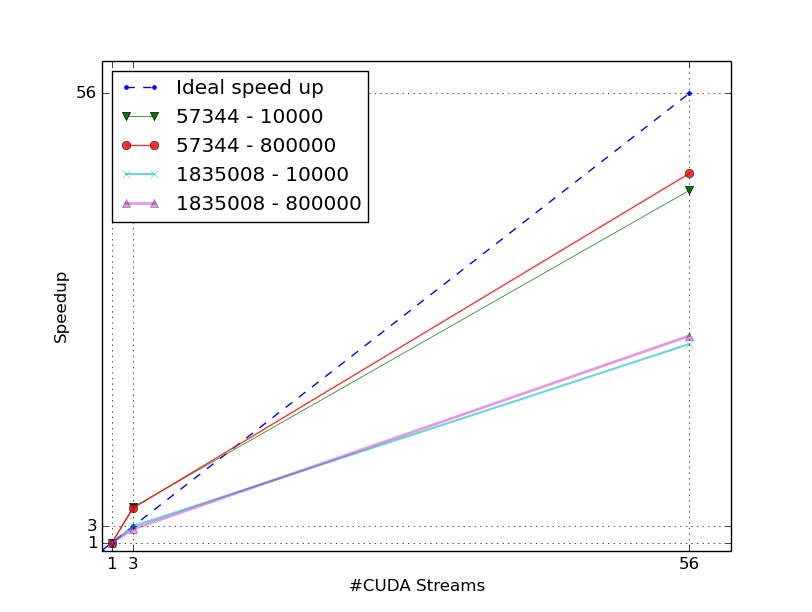
\includegraphics[scale=0.7]{plots/figure_25.png}
		\caption{Speedup for 3 and 56 CUDA streams on P100 device.}
		\label{fig:p100sp}
	%\end{figure}
	% \vspace*{\floatsep}
	%\begin{figure}
		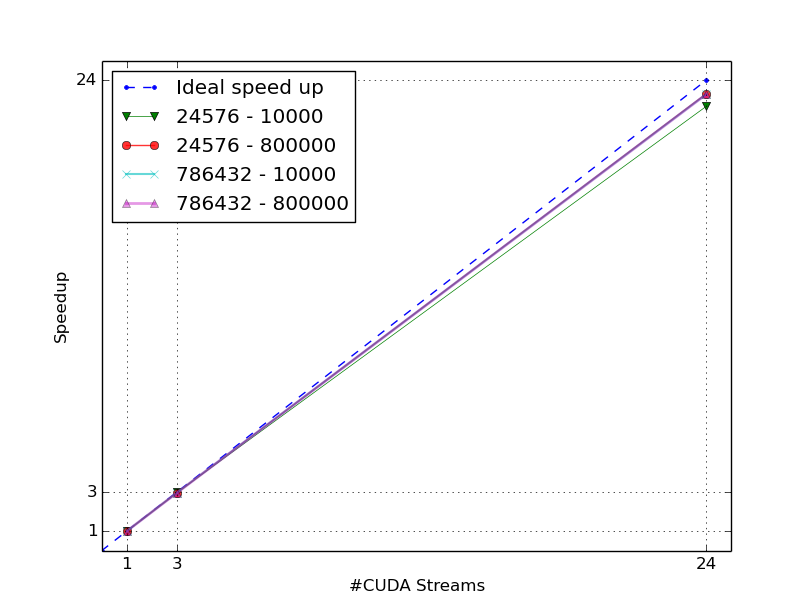
\includegraphics[scale=0.7]{plots/figure_26.png}
		\caption{Speedup for 3 and 56 CUDA streams on M40 device.}
		\label{fig:m40sp}
	\end{figure}
	To have an overall view on speedup we also present plots for both P100, in  \hyperref[fig:p100sp]{Figure 5.1}, and M40, in \hyperref[fig:m40sp]{Figure 5.2}.\\
	The two plots show the speedups only for a part of the real input dataset; in particular, each plot shows the smaller and bigger input stream length and for both it shows the smaller and bigger kernel iterations number.
	
	From the two plots we can clearly see how performances increase proportionally to the number of CUDA streams\footnote{More precisely this gain is bounded to the number of Streaming Multiprocessors the GPU exploits.}.
			
			
	{\large \textbf{Bigger buffers}}\\\\
			All relative measures to 2048 items buffers are reported in Table ***
%\end{enumerate}


%%%%%%%%%%%%%%%%%%%
%%%%% MAT MUL %%%%%
%%%%%%%%%%%%%%%%%%%
\section{Matrix Multiplication}
With Matrix multiplication we're facing a kernel mostly memory-bound, so we had to make some slightly different tests with respect to the ones in simple-computation kernel.\\
Note that, even if the logic is the same as the previous application, there are some details to redefine.\\
First of all, before we were dealing with an input stream of floats that were accumulated in buffers, here we have an input stream of matrices. In particular as soon as we have two available input matrices, they're sent out to device to apply the matrix multiplication kernel. Finally we get back to host with the result matrix, that will be one of the output stream components.

Another assumption is that, for simplicity, we're measuring on square matrices case, even if code was implemented for non-square case too. \\
Thus we performed the following executions:
%BLOCK=32
%matSize=(128 512 1024)
%#nStreams=(0 3 56)
%nMats=(256 1024 2048) # 14680064 29360128)
%dpSize=(2048 3840 5504 7680 8192 15360)

	\begin{table}	
		\centering
		\begin{tabular}{| c | c | c | c |} 
			\hline
			
			 \multicolumn{2}{c}{\textbf{Tesla P100}} & \multicolumn{2}{c}{\textbf{Tesla M40}} \\ [0.5ex]
			 % & \textbf{Tesla P100} & \textbf{Tesla M40} \\ 
			\hline\hline
			
			\textbf{Mat. Order} & \textbf{In stream limit} & \textbf{Mat. Order} & \textbf{In stream limit}  \\ 
			\hline
			128 & 225 & 64 & 100  \\ 
			\hline	
			256 & 441 & 128 & 196  \\ 
			\hline	
			512 & 900 & 256 & 400  \\ 
			\hline		
			1024 & 1764 & 512 & 784  \\ 
			\hline			
			2048 &  & 1024 &  \\
			\hline
			\hline				
			%3 670 016 & ---- & ---- & ---- \\
			%\hline
			
			\multicolumn{2}{c}{Data Parallel} &  \multicolumn{2}{c}{Data Parallel} \\ [0.5ex]
			% & \textbf{Data Parallel} & \textbf{Data Parallel} \\ 
			\hline\hline
			\multicolumn{2}{c}{1920} & \multicolumn{2}{c}{1280} \\ [0.5ex]
			% & \textbf{Data Parallel} & \textbf{Data Parallel} \\ 
			\hline			
			\multicolumn{2}{c}{2816} & \multicolumn{2}{c}{1792} \\ [0.5ex]
			\hline
			\multicolumn{2}{c}{3840} & \multicolumn{2}{c}{2560} \\ [0.5ex]
			\hline
			\multicolumn{2}{c}{5632} & \multicolumn{2}{c}{3584} \\ [0.5ex]
			\hline
			\multicolumn{2}{c}{7680} & \multicolumn{2}{c}{5120} \\ [0.5ex]
			\hline
			\multicolumn{2}{c}{11264} & \multicolumn{2}{c}{7168} \\ [0.5ex]
			\hline

		\end{tabular}
		\caption{Input dataset for Matrix Multiplication kernel. Above Stream parallel configuration, below Data Parallel correspondent.}	
		\label{tab:matdata}		
	\end{table}
	
\begin{enumerate}
	\item \textbf{Classic data parallel approach}
	As always we have to put a limit on input stream, so that we can measure completion times and compare different approaches.\\
	To test the data parallel version it suffices to treat input/output streams as huge matrices.
	This means that we'll do computations, no longer on stream of small data structures, but on a unique big data structure.\\
	So, for example:
	\begin{itemize}
		\item We have two input streams, each has limit to 9 square matrices of order 2 (one input stream is for \textbf{A} matrices and one for \textbf{B});
		\item So suppose that our stream parallel model, sends out one matrix A and one B at time;
		\item Then we launch the kernel, performing the matrix multiplication, this will give back a matrix result C;
		\item This means in total we will perform 9 multiplications between couples of matrices, giving 9 result matrices;
		\item If we consider those 9 small matrices as block matrices, we can combine them into a bigger one;
		\item This will be equivalent to pick A and B matrices each of order 6;
		\item note that, for simplicity, we'll choose as input stream limit a square number, so that the equivalent combined data structure will be again square;
		\item In our example 9 is a square number so that we can obtain as composed matrix dimension \([(2\cdot3)\times(2\cdot3)] = [6\times6]\)  
	\end{itemize} 
	In \hyperref[tab:matdata]{Table 5.2}, in the lower portion, are showed the matrices orders we used to test data parallel version for matrix multiplication. 
	By giving these values as (square) matrix dimension and computing only one multiplication between matrices, we'll get the relative comparison to some Stream parallel versions \footnote{We'll see later what cases we match between data and stream parallel to make comparisons.}.
	
	\item \textbf{Streaming parallel}
	As we mentioned before, we have to put a limit on the stream length for both streams of input matrices.\\
	In the upper portion of \hyperref[tab:matdata]{Table 5.2} are reported all input stream limit, for each of them we test all of matrices order.\\
	For every combination given by the input dimensions, we'll test for different numbers of CUDA streams: \textbf{Zero}, \textbf{Three} and \textbf{N\textsubscript{SM}} CUDA Streams (with \(N_{SM} \ =\# Streaming \ Multiprocessors\)).
	The above test on different numbers of non-default streams, is implemented in a totally analogous way to the one for Simple-computation Kernel. And the reasons why we test for those numbers of streams are the same too.
\end{enumerate}



\subsection{Results}
\begin{table}	
	\centering
	\begin{tabular}{ | c c c  | c c c | } 
		\hline
		\multicolumn{3}{c}{\textbf{Tesla P100 (zero Streams)}} & \multicolumn{3}{c}{\textbf{Tesla M40 (zero Streams)}}\\ [0.5ex]
		% & \textbf{Tesla P100} & \textbf{Tesla M40} \\ 
		\hline\hline
		Event Times  & Number of Mats & Mat. Order & Event Times  & Number of Mats & Mat. Order  \\
		\hline
		
		
		86.8854&	225&	\multirow{4}{*}{128}&	17.4869&	100&	\multirow{4}{*}{64}\\
		175.189&	441&	&	34.8778&	196&	\\
		359.9716&	900&	&	70.9718&	400&	\\
		725.5573&	1764&	&	139.3896&	784&	\\
		\hline
		334.0376&	225&	\multirow{4}{*}{256}&	36.2095&	100&	\multirow{4}{*}{128}\\
		672.9463&	441&	&	74.2685&	196&	\\
		1435&	900&	&	147.7336&	400&	\\
		2828.5366&	1764&	&	299.138&	784&	\\
		\hline
		1673.2133&	225&	\multirow{4}{*}{512}&	186.3913&	100&	\multirow{4}{*}{256}\\
		3325.6533&	441&	&	368.6813&	196&	\\
		6611.7566&	900&	&	786.7536&	400&	\\
		12919.6666&	1764&	&	1603.4933&	784& \\
		\hline
		10998.7666&	225&	\multirow{4}{*}{1024}&	1256.4&	100&	\multirow{4}{*}{512}\\
		21511.1666&	441&	&	2479.4333&	196&	\\
		43828.7666&	900&	&	5162.6333&	400&	\\
		85853.0333&	1764&	&	9791.98&	784&	\\
		\hline
		80764.8666&	225&	\multirow{4}{*}{2048}&	9075.22&	100&	\multirow{4}{*}{1024}\\
		158136.3333& 441&	&	17849.5666&	196&	\\
		309724.6666& 900&	&	36441.3666&	400&	\\
		604324&	1764&	&	72396.8666&	784&	\\
		
		\hline
		
	\end{tabular}
	\caption{Device completion times for Mat-Mul kernel, without using CUDA Streams (zero streams), results are reported for both P100 and M40.}	
	\label{tab:matvgszero}		
\end{table}

\begin{table}	
	\centering
	\begin{tabular}{ | c c c  | c c c | } 
		\hline
		\multicolumn{3}{c}{\textbf{Tesla P100 (zero Streams)}} & \multicolumn{3}{c}{\textbf{Tesla M40 (zero Streams)}}\\ [0.5ex]
		% & \textbf{Tesla P100} & \textbf{Tesla M40} \\ 
		\hline\hline
		Event Times  & Number of Mats & Mat. Order & Event Times  & Number of Mats & Mat. Order  \\
		\hline

		25.5549& 225&	\multirow{4}{*}{128}&	5.2046&	100&	\multirow{4}{*}{64}\\
		53.2203&	441&	&	10.7422&	196&	\\
		102.0575&	900&	&	23.9773&	400&	\\
		193.2436&	1764&	&	47.1808&	784&	\\
		\hline
		148.1446&	225&	\multirow{4}{*}{256}&	21.5294&	100&	\multirow{4}{*}{128}\\
		289.6773&	441&	&	41.9395&	196&	\\
		590.6776&	900&	&	74.5879&	400&	\\
		1157&	1764&	&	143.3123&	784&	\\
		\hline
		1173.3466&	225&	\multirow{4}{*}{512}&	129.985&	100&	\multirow{4}{*}{256}\\
		2298.3866&	441&	&	254.2516&	196&	\\
		4690.97&	900&	&	518.3303&	400&	\\
		9205.5&	1764&	&	1016.28&	784&	\\
		\hline
		9371.7766&	225&	\multirow{4}{*}{1024}&	1033.9166&	100&	\multirow{4}{*}{512}\\
		18371.2666&	441&	&	2027.17&	196&	\\
		37480.4&	900&	&	4136.54&	400&	\\
		73258.6666&	1764&	&	8113.0933&	784&	\\
		\hline
		74966.4666&	225&	\multirow{4}{*}{2048}&	8273.1066&	100&	\multirow{4}{*}{1024}\\
		146156.3333&	441&	&	16194.1&	196&	\\
		285788.3333&	900&	&	33041.1&	400&	\\
		559469.6666&	1764&	&	64763.6666&	784&	\\
		
		\hline
		
		
	\end{tabular}
	\caption{Device completion times for Mat-Mul kernel, with three CUDA Streams, results are reported for both P100 and M40.}	
	\label{tab:matvgsThree}		
\end{table}


\begin{table}	
	\centering
	\begin{tabular}{ | c c c  | c c c | } 
		\hline
		\multicolumn{3}{c}{\textbf{Tesla P100 (zero Streams)}} & \multicolumn{3}{c}{\textbf{Tesla M40 (zero Streams)}}\\ [0.5ex]
		% & \textbf{Tesla P100} & \textbf{Tesla M40} \\ 
		\hline\hline
		Event Times  & Number of Mats & Mat. Order & Event Times  & Number of Mats & Mat. Order  \\
		\hline
		
		
		%86.8854&	225&	\multirow{4}{*}{128}&	17.4869666667&	100&	64\\
		20.8758&	225&	\multirow{4}{*}{128}&	2.739&	100&	\multirow{4}{*}{64}\\
		40.5783&	441&	&	5.0942&	196&	\\
		74.6636&	900&	&	10.0277&	400& \\
		145.4766&	1764&	&	19.8252&	784&	\\
		\hline
		147.765&	225& \multirow{4}{*}{256}&	19.3538&	100&	\multirow{4}{*}{128}\\
		288.5343&	441&	&	37.8560&	196&	\\
		588.9643&	900&	&	65.6809&	400&	\\
		1153.7333&	1764&	&	128.317&	784&	\\
		\hline
		1173.32&	225&\multirow{4}{*}{512}&	130.0533&	100&	\multirow{4}{*}{256}\\
		2298.3966&	441&	&	254.281&	196&	\\
		4690.9633&	900&	&	518.615&	400&	\\
		9202.3333&	1764&	&	1016.55&	784&	\\
		\hline
		9371.0433&	225&	\multirow{4}{*}{1024}&	1034.0666&	100&	\multirow{4}{*}{512}\\
		18374.7&	441&	&	2027.2866&	196&	\\
		37474.7&	900&	&	4136.7066&	400&	\\
		73348.3333&	1764&	&	8110.9966&	784&	\\
		\hline
		74971.6666&	225&	\multirow{4}{*}{2048}&	8262.7533&	100&	\multirow{4}{*}{1024}\\
		146175.6666&	441&	&	16202.4666&	196&	\\
		285955.6666&	900&	&	33059.2666&	400&	\\
		559425&	1764&	&	64786.5333&	784&	\\
		
		\hline
		
		
	\end{tabular}
	\caption{Device completion times for Mat-Mul kernel, with as many CUDA Streams as SM number, results are reported for both P100 and M40.}	
	\label{tab:matvgsSM}		
\end{table}






All the above tests on Matrix Multiplication Kernel give us the measures of device times.\\
Below we'll see that completion times and performance will notably be different, with respect to the previous computation-bound application.

All collected elapsed times are reported in \hyperref[tab:matvgszero]{Table 5.6}, for the zero-streams version, in \hyperref[tab:matvgsThree]{Table 5.7}, for the three-streams one, and \hyperref[tab:matvgsSM]{Table 5.8}, for the SM-streams version.\\
From these tables we can highlight some behaviors:
\begin{itemize}
	\item input streams of matrices have lengths that grow by a factor of 2 and it's easy to see that this makes a proportional increase in completion times, ie even measures grows by factors of 2;
	
	\item input matrix sizes again grow of 2x each, but in this case the completion times don't grow proportionally;
	
	\item for zero-streams we can see that, as the matrix order grows by a factor of 2, the completion time can increase from \~4x to \~7x; 
	
	\item for three-streams we can see that, as the matrix order grows by 2x, the completion time can increase from \~5x to \~7.9x; 
	
	\item finally for SM-streams we can see that, the completion time can increase from \~7x to \~8x.
\end{itemize}
Those evidences holds for both machines measures and they give some hints on matrix multiplication behavior.\\
The first point tells us that elapsed time to send/receive to/from the device grows linearly with the number of matrices, so this input variable would not affect performances. Especially, no matter the CUDA streams amount we decide to use, the increase by 2x of matrices quantity, will always give a growth of 2x in measures.

The other points tells us that, as matrix order increases, we'll get worser and worser performances. Clearly this doesn't depend on CPU/GPU data transfers overhead \footnote{Host/device transfers, in general, give a bigger overhead when lot of calls are issued.}, otherwise we'd have the same behavior when number of matrices grows.\\
So, the cause must reside exclusively on what happens inside the GPU. In reality, the classic matrix multiplication is a well known problem in GPUs paradigm and it's also known as a not-so-efficient problem. \\
This is because, the simpler implementation, at each iteration, performs more \textit{global memory}/\textit{registers} transfers than effective calculations. So that's why this kind of matrix multiplication is considered memory-bound.\\
So, the more elements a matrices have, the more data transfers (internal to the device) the GPU will have to perform and the more active threads will stall waiting for data to be available for computations.\\

\begin{table}	
	\centering
	\begin{tabular}{ | c | c | c | c  || c | c | c | c | } 
		\hline
		\multicolumn{4}{c}{\textbf{Tesla P100 (56 Streams)}} & \multicolumn{4}{c}{\textbf{Tesla M40 (24 Streams)}}\\ [0.5ex]
		% & \textbf{Tesla P100} & \textbf{Tesla M40} \\ 
		\hline\hline
		\textbf{Mat. Number}  & \textbf{Mat. Order} & \textbf{Sp(3)} & \textbf{Sp(56)} & \textbf{Mat. Number}  & \textbf{Mat. Order}  & \textbf{Sp(3)} & \textbf{Sp(24)} \\
		\hline
		
		
		225& \multirow{4}{*}{128}&	3.3999&	4.1620&	100&	\multirow{4}{*}{64}&	3.3598&	6.3839\\
		441& &	3.2917&	4.3173&	196&	&	3.2467&	6.8464\\
		900& &	3.5271&	4.8212&	400&	&	2.9599&	7.0775\\
		1764& &	3.7546&	4.9874&	784&	&	2.9543&	7.0309\\
		\hline
		225& \multirow{4}{*}{256}&	2.2548&	2.2606&	100& \multirow{4}{*}{128}& 1.6818&	1.8709\\
		441& & 2.3230&	2.3322&	196& & 1.7708& 1.9618\\
		900& & 2.4294&	2.4364&	400& & 1.9806&	2.2492\\
		1764& &	2.4447&	2.4516&	784& & 2.0873&	2.3312\\
		\hline
		225& \multirow{4}{*}{512}&	1.4260&	1.4260&	100& \multirow{4}{*}{256}&	1.4339&	1.4331\\
		441& &	1.4469&	1.4469&	196&  & 1.4500&	1.4498\\
		900& &	1.4094&	1.4094&	400& &	1.5178&	1.5170\\
		1764& &	1.4034&	1.4039&	784& &	1.5778&	1.5773\\
		\hline
		225& \multirow{4}{*}{1024}&	1.1736&	1.1736&	100&	\multirow{4}{*}{512}&	1.2151&	1.2150\\
		441& &	1.1709&	1.1706&	196& & 1.2231&	1.2230\\
		900& &	1.1693&	1.1695&	400& &	1.2480&	1.2480\\
		1764& &	1.1719&	1.1704&	784& &	1.2069&	1.2072\\
		\hline
		225& \multirow{4}{*}{2048}&	1.0773&	1.0772&	100&	\multirow{4}{*}{1024}&	1.0969&	1.0983\\
		441& &	1.0819&	1.0818&	196& &	1.1022&	1.1016\\
		900& &	1.0837&	1.0831&	400& &	1.1029&	1.1023\\
		1764& &	1.0801&	1.0802&	784& &	1.1178&	1.1174\\
		
		\hline
		
		
	\end{tabular}
	\caption{Here are showed speedups for all data sets of simple-computation kernel. Results are reported for both devices.}	
	\label{tab:matspeedup}		
\end{table}
So we'll now focus on speedups, to see that this memory-bound behavior will be reflected on our GPU Farm approach. All speedups are listed in \hyperref[tab:matspeedup]{Table 5.9}.\\
From those results, we can mainly observe that:
\begin{itemize}
	\item \textit{Sp(3)} gives results near to the expected value, ie \~3 for the smaller matrix sizes (128-256 for the P100, 64 for the M40);
	
	\item 	\textit{Sp(SM)} gives a really poor gain w.r.t. \textit{Sp(3)};
	
	\item all speedups degrade  to \~1 as the matrix order grows.
\end{itemize}




%\begin{figure}
%	\vspace{-1.5cm}
%	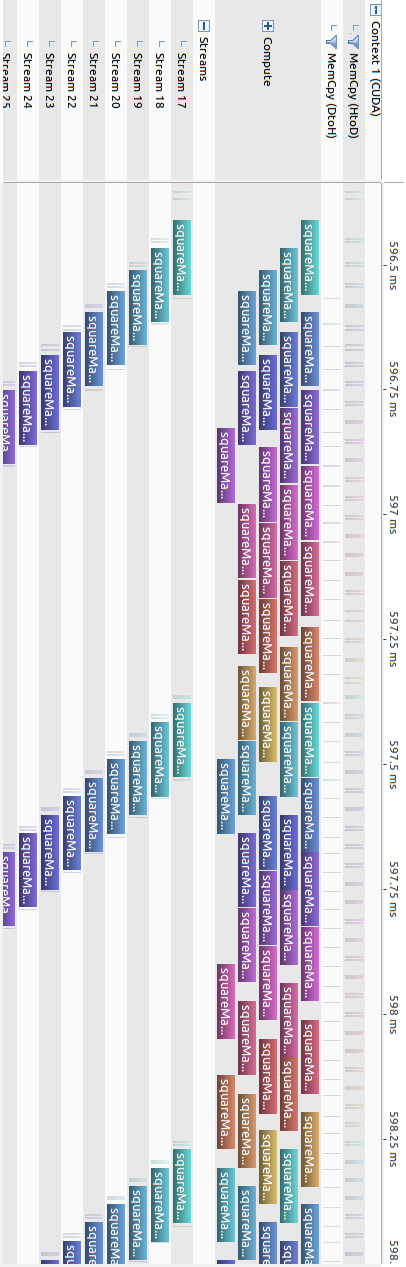
\includegraphics[scale=0.7]{plots/matmul784_64_timeline.png}
%	\caption{NVIDIA Visual profiler generated \textit{timeline} on M40, using 24 CUDA streams and running code for 784 matrices of size 64.}
%	\label{fig:mat64timeln}
%\end{figure}

% \vspace*{\floatsep}
%\begin{figure}
%	\vspace{-1.5cm}
%	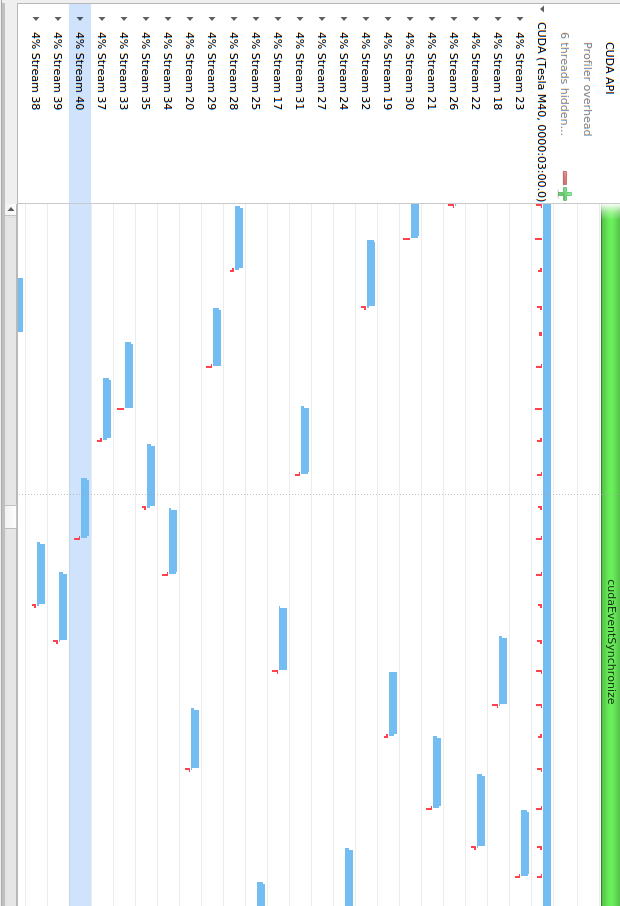
\includegraphics[scale=0.7]{plots/mat_big_str_nsight.png}
%	\caption{Nsight profiler execution on M40, using 24 CUDA streams and running code for 784 matrices of size 256.}
%	\label{fig:matnsightbig}
%\end{figure}

%\begin{figure}[!tbp]
%	\centering
%	\vspace{-1.5cm}
%	\begin{minipage}[b]{0.1\textwidth}
%		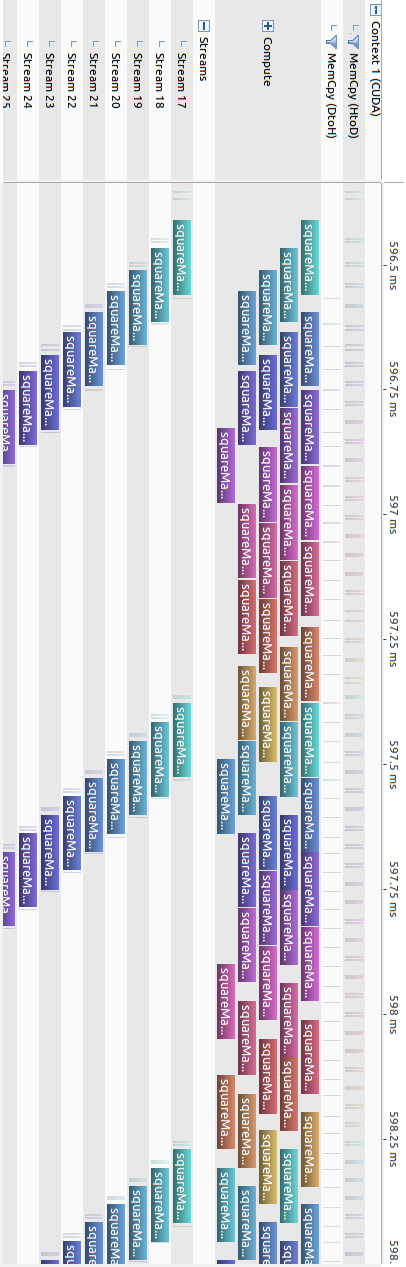
\includegraphics[scale=0.5]{plots/matmul784_64_timeline.png}
%		\caption{NVIDIA Visual profiler generated \textit{timeline} on M40, using 24 CUDA streams and running code for 784 matrices of size 64.}
%		\label{fig:mat64timeln}
%	\end{minipage}
	
	%\vfill
%	\begin{minipage}[b]{0.4\textwidth}
%		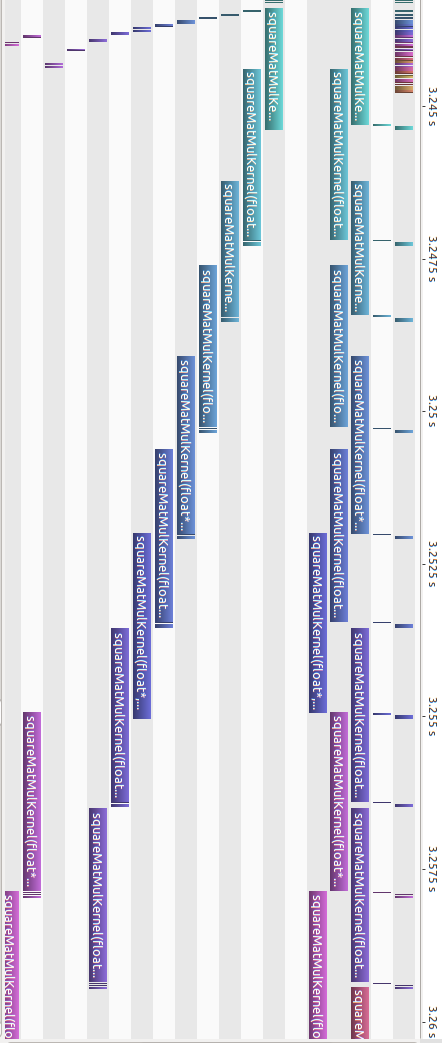
\includegraphics[scale=0.5]{plots/matmul784_256_timeline.png}
		%\caption{Same,except for matrices size set to 256.}
		%\label{fig:mat256timeln}
%	\end{minipage}
	%\hfill
%	\begin{minipage}[b]{0.4\textwidth}
%		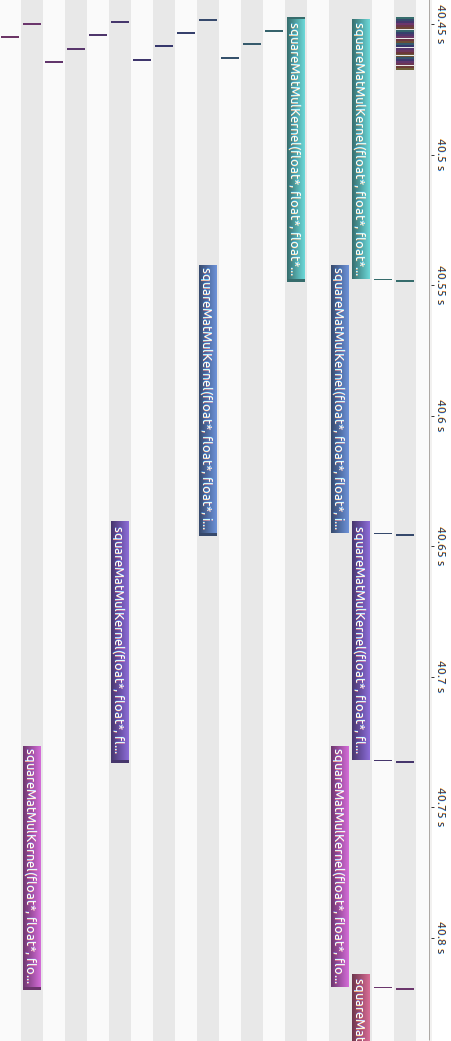
\includegraphics[scale=0.5]{plots/matmul784_1024_timeline.png}
		%\caption{Same,except for matrices size set to 1024.}
		%\label{fig:mat1024timeln}
%	\end{minipage}
	
%\end{figure}



%\begin{figure}[!tbp]
%	\centering
%	\vspace{-1cm}
	%\raggedright
%	\subfloat[Matrix size 64]{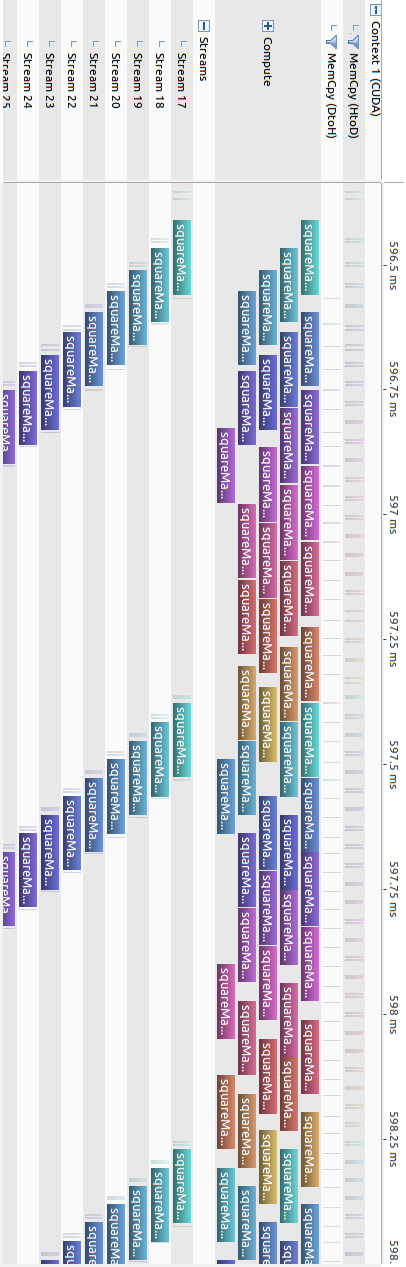
\includegraphics[width=0.4\textwidth]{plots/matmul784_64_timeline.png}\label{fig:timeln64}}
%	\raggedleft
%	\hfill
%	\subfloat[Matrix size 256]{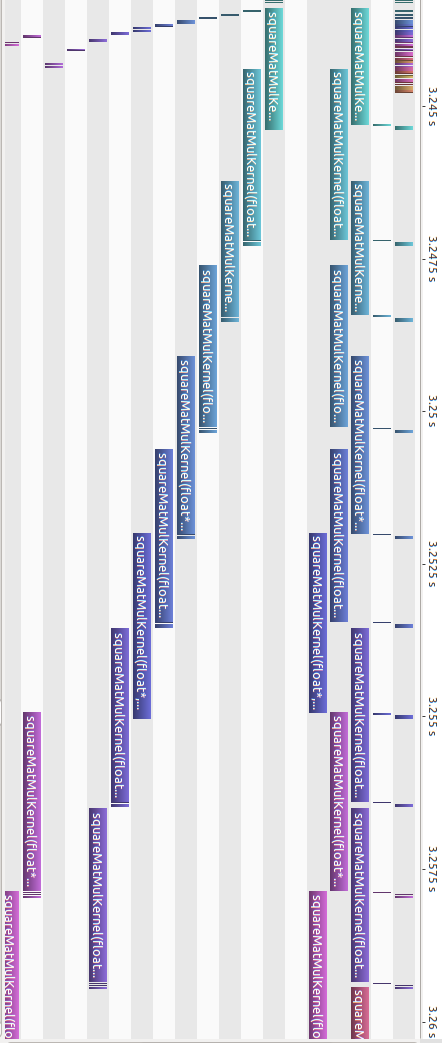
\includegraphics[width=0.2\textwidth]{plots/matmul784_256_timeline.png}\label{fig:timeln256}}
%	\vfill
%	\subfloat[Matrix size 1024]{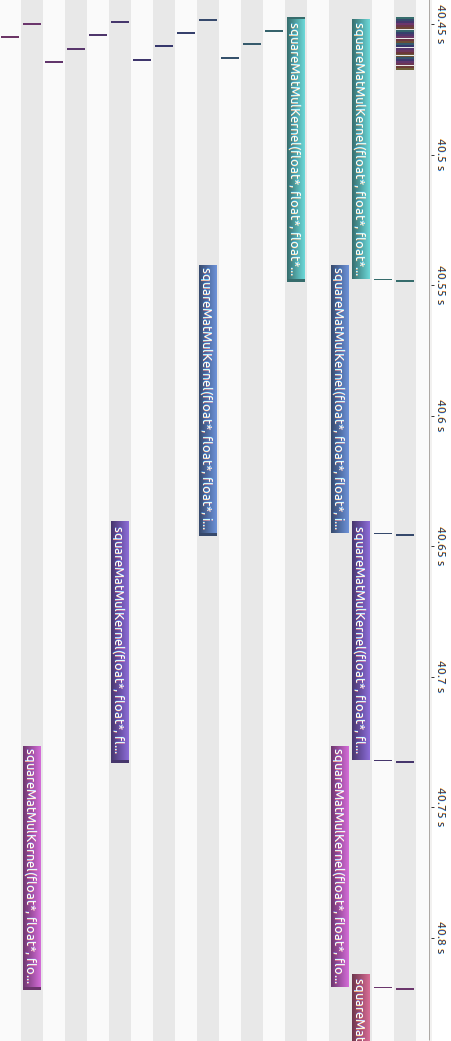
\includegraphics[width=0.2\textwidth]{plots/matmul784_1024_timeline.png}\label{fig:timeln1024}}
%	\caption{NVIDIA Visual profiler generated \textit{timeline} on M40, using 24 CUDA streams and running code for 784 matrices.}
%\end{figure}

\begin{figure}[!tbp]
	\centering
	\vspace{-1cm}
	\hspace{2cm}
	\begin{tabular}[c]{cc}
		\makecell[tl]{\subfloat[Matrix size 256]{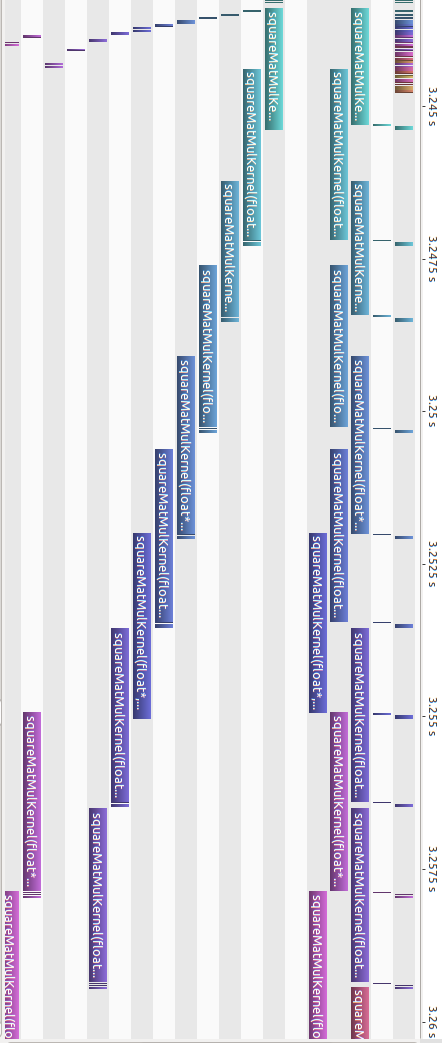
\includegraphics[width=0.32\textwidth]{plots/matmul784_256_timeline.png}\label{fig:timeln256}} \\
		\subfloat[Matrix size 1024]{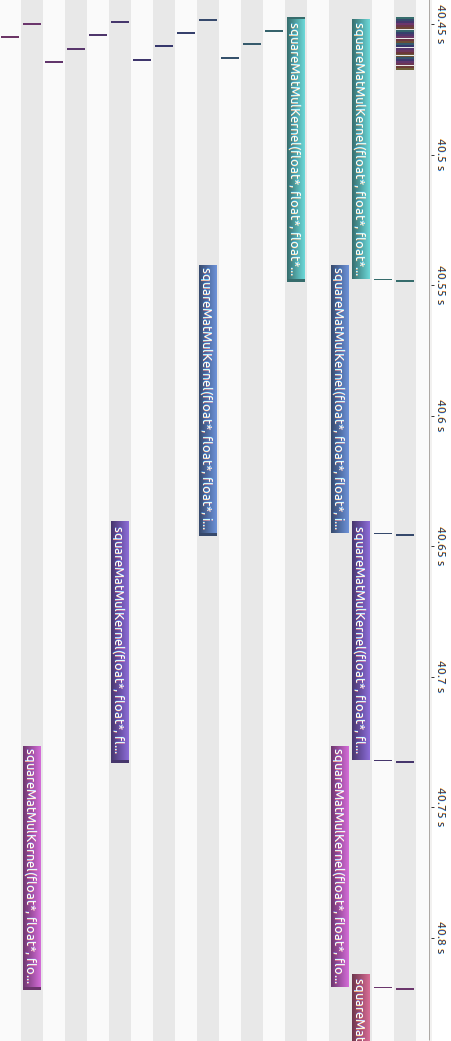
\includegraphics[width=0.32\textwidth]{plots/matmul784_1024_timeline.png}\label{fig:timeln1024}}}
		& \vspace*{2cm}
		\subfloat[Matrix size 64]{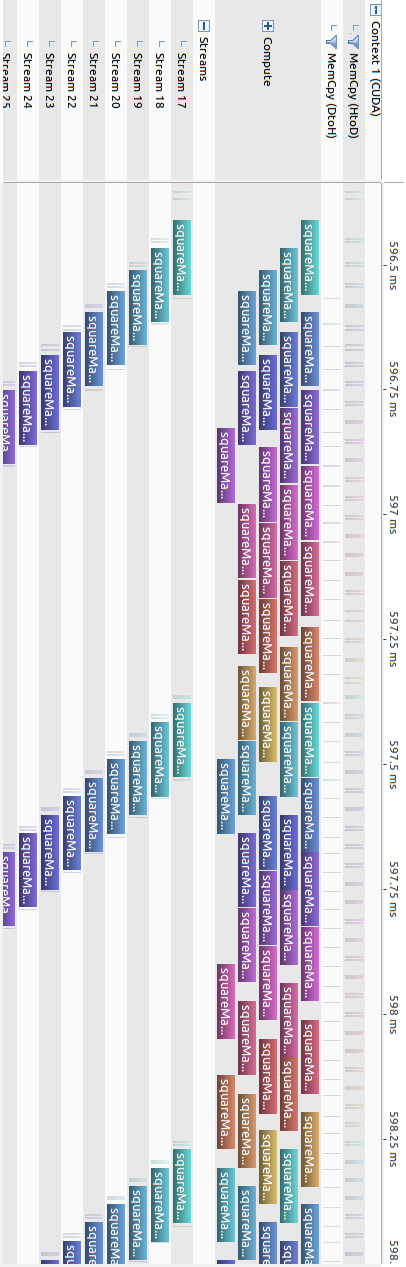
\includegraphics[width=0.45\textwidth]{plots/matmul784_64_timeline.png}\label{fig:timeln64}}\\
		
	%	\subfloat[Matrix size 1024]{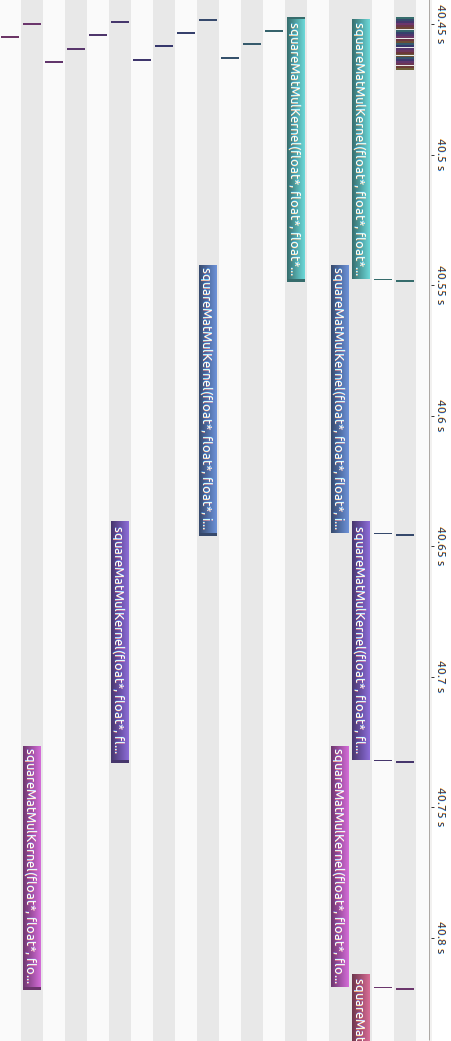
\includegraphics[width=0.2\textwidth]{plots/matmul784_1024_timeline.png}\label{fig:timeln1024}} &\vspace*{1cm} \\
	\end{tabular}    
	\caption{NVIDIA Visual profiler generated \textit{timeline} on M40, using 24 CUDA streams and running code for 784 matrices.}
	\label{fig:timeln}
\end{figure}

This behavior translates in the following: when the matrices get bigger, even if CUDA Streams push to have more simultaneous mat-mul, we'll have a lot of active threads (and so Multiprocessors) busy and probably mainly stalled on gathering floats from global memory.\\
This, in fact, inevitably leads to a very limited amount of gain, even when using a lot of CUDA streams. Furthermore, those results tells us that we will fit in Multiprocessor less matrix multiplication than we expect \footnote{Clearly this holds strictly for the type of matrix multiplication we implemented.}.\\
Profiling the application for some key data set we can inspect the above described facts and the relative reasons.

\begin{figure}[!tb]
	\centering
	\vspace{-2cm}
	%\hspace{2cm}
	\begin{tabular}[c]{cc}
		\multicolumn{2}{c}{\subfloat[Matrix size 64]{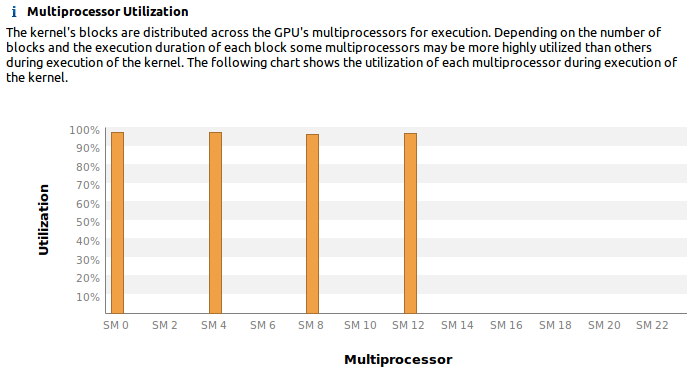
\includegraphics[width=\textwidth]{plots/matmul784_64_SMuse.png}\label{fig:SMuse64}}} \\
		
		\subfloat[Matrix size 1024]{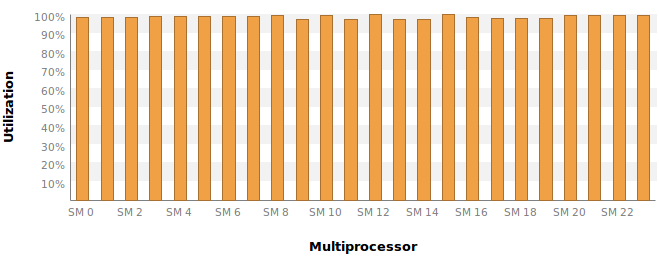
\includegraphics[width=0.5\textwidth]{plots/matmul784_1024_SMuse.png}\label{fig:SMuse1024}}
		&
		\subfloat[Matrix size 256]{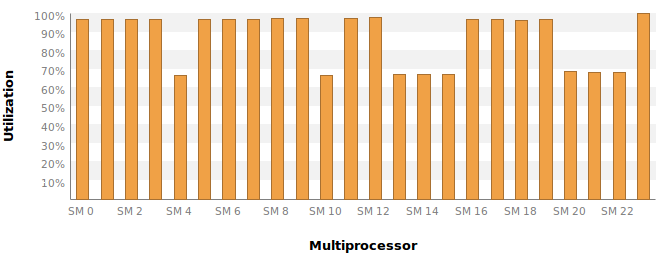
\includegraphics[width=0.5\textwidth]{plots/matmul784_256_SMuse.png}\label{fig:SMuse256}}\\
		
		%	\subfloat[Matrix size 1024]{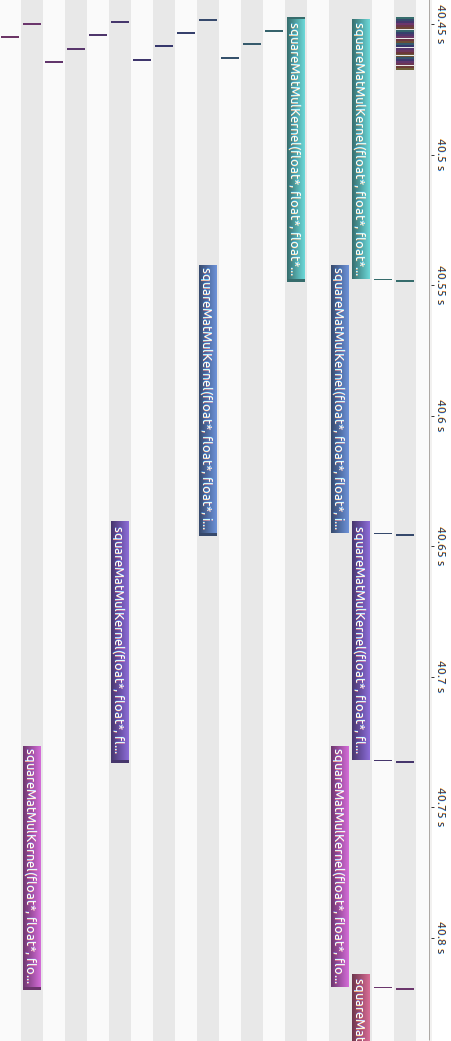
\includegraphics[width=0.2\textwidth]{plots/matmul784_1024_timeline.png}\label{fig:timeln1024}} &\vspace*{1cm} \\
	\end{tabular}    
	\caption{NVIDIA Visual profiler generated \textit{timeline} on M40, using 24 CUDA streams and running code for 784 matrices.}
	\label{fig:SMuse}
\end{figure}

In \hyperref[fig:timeln]{Figure 5.3} we can have a visual cue on what is happening during an execution of mat-mul on M40, with 24 CUDA streams, having an input stream of 784 matrices of sizes: 64x64 (\hyperref[fig:timeln64]{Figure 5.3}), 256x256(\hyperref[fig:timeln256]{Figure 5.3}), 1024x1024(\hyperref[fig:timeln1024]{Figure 5.3}).\\
%In this screen shot on top there's the timeline of all CUDA APIs that have been called, under that we find a light blue line representing all kernel activities in M40 and attached below there are lot of red ticks that shows all memory copy activities (from host to device and viceversa).\\
Analyzing the figure we can see that the amount of overlapping between operations in different streams is quite limited in general, this just confirms what we saw from speedups.\\
From the above pictures, we can observe that in 64-sized case we're having a slightly better overlapping and a little more kernels running at the same time. In this case this may happens for few reasons:
\begin{itemize}
	\item grid and block sizes are smaller for each kernel launch, so this allow to have multiple kernels fit in SMs;
	\item kernel durations are shorter so this gives a further chance to overlap data transfers, other than kernel.
\end{itemize} 

A 64x64 result matrix (say C) is managed by a grid of 2x2 blocks, each of which has 32x32 threads\footnote{This depends on how we implemented kernel launch, that is the classical kernel launch approach setting blocks at the maximum size possible. Remember implementations in \hyperref[chap:impl]{Chapter 4}}, while a 256x256 C is managed by a grid of 8x8 blocks, each of which having 32x32 threads and, finally, a 1024x1024 C is managed by a grid of 32x32 blocks, each of which having 32x32 threads.\\
This means that, in the two latter cases, we don't even have all blocks of a kernel launch fitting in all the SMs. If this may theoretically give a full occupancy of the GPU by a certain kernel, from the other side means saturate the cores without permitting other launches to fit, until the residing kernels ends or, at least, some resources are available.

We can confirm this fact by looking at the occupancy graphs (generated from Visual Profiler), showed in \hyperref[fig:SMuse]{Figure 5.4}. In 64-sized case we've only 4 SMs almost fully employed, while in the other cases all SMs are almost busy.\\
The above cases exposes an example of the fact that \textit{not always a high or full occupancy may give better performances} \cite{loweroccupancy,cudabestpractices}, it strongly depends on the kernel nature.\\
On the other side as we decrease the matrices size we can't exploit enough resources. As we can see from \hyperref[fig:timeln64]{Figure 5.3} we have a better overlapping, but it seems that kernels lasts too little, so the host can't push kernels quickly enough to fill SMs. In fact Visual Profiler suggests us that those kernels perform a really poor amount of computations, especially with respect to memory latencies, see figure \hyperref[fig:mat62latency]{Figure 5.5}.\\ 
\begin{figure}[!tb]
	%\centering
	\vspace{-1cm}
	\hspace{-1cm}
	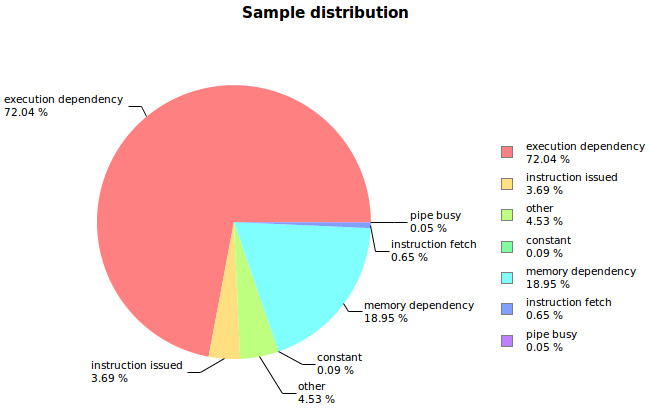
\includegraphics[scale=0.8]{plots/matmul784_64_kerlatencies.png}
	\caption{Nsight profiler execution on M40, 24 CUDA streams, 784 matrices of size 256. This graph gives the types and relative amounts of latencies inside our mat-mul kernel code.}
	\label{fig:mat62latency}
\end{figure}
This pie chart shows that most of the time kernels is idle on:
\begin{itemize}
	\item execution dependency\footnote{Execution dependency stall can be potentially reduced by increasing instruction-level parallelism Instruction-Level Parallelism, a.k.a. ILP, means that we can improve parallelism by increasing the amount of instructions for each thread. This can translate in less threads having a greater work-load each. }, ie an input required by the issued instruction isn't yet available; 
	
	\item memory dependency\footnote{ Memory dependency stall type can potentially be reduced by optimizing memory alignment and access patterns}, a load/store cannot be made because the required resources aren't available or are fully utilized, or too many requests of a given type are outstanding.
\end{itemize}
This demonstrates the fact that matrix multiplication is a memory-bound problem in GPU and, so,poor in computation amount.\\
This is why we have really short kernels for small input data size and heavy kernels for bigger input sizes.


%%%%%%%%%%%%%%%%%%%%%%
%%%%% IMAGE PROC %%%%%
%%%%%%%%%%%%%%%%%%%%%%
\section{Image processing}
With image processing, ie Blur Box algorithm we're facing a kernel mostly memory-bound and especially rich of divergent execution flows, so we made similar tests to the ones for Matrix multiplication.\\
Thus we performed the following executions:
%BLOCK=1024
%imgSize=(128 256)
%#nStreams=(0 3 56)
%nImgs=(256 1024) # 14680064 29360128)
%dpSize=(4096 8192)


\begin{table}	
	\centering
	\begin{tabular}{| c | c |} 
		\hline
		
		 \multicolumn{2}{c}{\textbf{Tesla P100} \& \textbf{Tesla M40}} \\ [0.5ex]
		%& \textbf{Tesla P100} & \textbf{Tesla M40} \\ 
		\hline\hline
		
		\textbf{Img. Order} & \textbf{In stream limit} \\ 
		\hline
		128 & 64 \\ 
		\hline		
		256	& 256 \\ 
		\hline			
		512	& 1024 \\ 
		\hline	
		\hline
			

	\multicolumn{2}{c}{\textbf{Data Parallel Tesla P100 \& Tesla M40}} \\ [0.5ex] 
		\hline\hline		
		\multicolumn{2}{c}{1024 \((=128\cdot8)\)} \\ [0.5ex] 
		
		
		
		\multicolumn{2}{c}{2048 \((=128\cdot32)\)} \\ [0.5ex] 
		
		\multicolumn{2}{c}{4096 \((=128\cdot32)\)} \\ [0.5ex] 
		
		\multicolumn{2}{c}{8192 \((=256\cdot32)\)} \\ [0.5ex] 
		\hline
		
		
	\end{tabular}
	\caption{Input dataset for Image Processing kernel. Above Stream parallel configuration, below Data Parallel correspondent.}	
	\label{tab:imgdata}		
\end{table}

\begin{enumerate}
	\item \textbf{Classic data parallel approach}
	If we think to a picture as a matrix of pixels, then it's easy to see the analogy to the previous application.\\
	In particular the Data Parallel approach will be tested giving an image of large dimensions, instead of a stream of small images.\\
	Again we can consider a single big image, as formed by merging smaller ones. Similarly to matrix multiplication case we chose, as input stream limits, square numbers to make possible a balanced comparison to the correspondent square picture in data parallel.\\
	In the lower part of \hyperref[tab:imgdata]{Table 5.3} we show the order of dimension of the images used to compare to some streaming parallel cases.
	
	\item \textbf{Streaming parallel}
	
	As previous cases of Farm parallel pattern, we have to put a limit on the stream length for input stream of images.\\
	In the upper portion of \hyperref[tab:imgdata]{Table 5.3} are reported input stream limits, for each of them we test the two types of picture dimensions. Note that those images are square, so, for example, a size of 128 stands for a picture of \((128\times128)\) resolution (ie 16 384 pixels).\\
	For every combination given by the input dimensions, we'll test for different numbers of CUDA streams: \textbf{Zero}, \textbf{Three} and \textbf{N\textsubscript{SM}} CUDA Streams (with \(N_{SM} \ =\# Streaming \ Multiprocessors\)).
	The above test on different numbers of non-default streams, is implemented in a totally analogous way to the ones for the two applications showed above.
	
	\begin{itemize}
		\item \textbf{Zero} CUDA Streams
		\item \textbf{Three} CUDA Streams
		\item \textbf{N} CUDA Streams, with \(N=\# of Streaming Multiprocessors\)
	\end{itemize}
\end{enumerate}



\subsection{Results}
As expected this image processing kernel demonstrates a really bad fitting in Farm parallel pattern for GPU. This is because it gives even worst performances than matrix multiplication.

We report in \hyperref[tab:imgdata]{Table ***} all completion times, for zero-streams, three-streams and SM-streams versions.\\
We can see that the input stream of images grows in length by a factor of 4, in fact completion times follow this trend by increasing ~4x proportionally with input limits.\\
Instead, fixed a certain number of images as input stream limit, the image size grows by a factor of 2. This time this lead to an increasing of completion times by a slightly bigger factor, ie ~3x.

But the really evident and important behavior is that we don't have much difference between the version not using CUDA Streams and the ones using them.\\
This is, in fact, confirmed by the speedups in \hyperref[tab:imgdata]{Table ***}, where we can see that almost everywhere the best speedup we can achieve is about 1.\\
This means that we almost have no overlapping, but we expected a similar behavior though.\\










\section{Results Summary}
Results are collected, for each group of execution, in some \texttt{.txt} files. In those files we can find a list of applications outputs in \texttt{.csv} format.

\subsection{Simple-computation kernel}
Dire che smaller buffer meglio perché non monopolizza interamente un SM, lascia spazio ad un altro kernel launch di entrare.

\subsection{Matrix Multiplication}
Dire che in sostanza si è capit oche per questo kernel e in versione Farm ci vuole un compromesso tra matrici grandi, quindi tanti blocchi, che saturano la GPU e matrici troppo piccole t.c il kernel dura troppo poco.
\subsection{Image Processing}


\section{Plots}
Plots
    \chapter{Conclusions} \label{chap:conclusions}
\setcounter{section}{1}
%\subsection{Overview and goals}
The main goal of this thesis was to experiment if a Farm parallel pattern could fit in GPU architecture and, if this was the case, how.\\
Even though a Streaming parallel pattern may seem so far from the classic GPU use, we founded our attempt on the increasing and pervasive concept of \textit{General-Purpose computing}.
Nowadays it's a common practice to use high parallelism and huge computational power of GPUs as co-processors, even if it isn't strictly for graphical problems.\\
Also the research moved, in last years, the focus on problems that generally are assigned to CPUs. Clearly, in General Purpose (GP) it's easy to spot applications that are clearly embarrassingly parallel; we recall that GPUs are known to be mostly suited for data parallel approaches.\\
However, there are many others problems that are really far from data parallel behavior and in some of those cases GP-GPUs demonstrate a fair behavior (generally with some proper adjustments).\\
So it makes perfectly sense to inspect for new non-data parallel applications to fit in GPU model. The main goal, in general, is to exploit the high computation potential of GPUs.


\subsection{Evaluation of the problem}
The starting point of this study was to consider and understand some main features and the functioning of a graphic processor, in particular taking into account of the organization about parallelism, threads, cores, internal memory and so on. We showed main GPUs and NVIDIA CUDA characteristics, briefly introducing them in \hyperref[chap:into]{Chapter 1} and deepening on more specific concepts in \hyperref[chap:tools]{Chapter 2} and \hyperref[chap:logic]{Chapter 3}.\\
In the latter we also showed how some best practices and considerations were exploited to evaluate and then design our model. \\

Once we had an overall view on tools and NVIDIA GPUs architecture, we had a base knowledge for the next step, i.e. to design a \textit{Farm parallel pattern} for a graphic processor. Obviously some key problems have arisen:
\begin{itemize}
	\item Handle the difference on input/output with respect to canonical data parallel problems, i.e. dealing with streams of data parallel tasks, instead of a single and purely data parallel structure;
	\item Manage the way we send data to device;
	\item Experiment several types of executions, each for different sizes of small data parallel tasks (from farm input stream);
	\item How to hide the overhead due to data transfers between host and device;
	\item How to execute many "small" kernels at the same time, instead of a single "big" one;
	\item How to exploit the resources of the GPU at their best, taking into account the studied application nature.
\end{itemize}
The first two points were accomplished by thinking to a \textit{particular way} to use CUDA streams and asynchronous host/device memory copies.\\
In other words, we decided to use many non-default streams, up to an high amount compared to the usual way CUDA streams are used.
This hopefully should have allowed us to hide data transfers and to be able to run, at the same time, a lot of "small" data parallel tasks on the several GPU multiprocessors.\\
Clearly we could expect to have different kernels running in parallel on the SMs, since tasks are arriving from a Farm stream, are supposed to be reasonably small to occupy a part of resources, without saturating too much SMs.
So this should allow more small tasks to fit in multiprocessors together.\\ 
%thinking to a system of \textit{accumulator buffers} that was sent to device as soon as they were filled by the input stream. This was mainly designed for the simple-computation kernel, but it applies to all those scenarios where we have an input stream made of simple items (eg floats, integers, etc.).\\
%Instead for the other two kernels we simply had to test the Farm parallel pattern on small matrices or small images, that straightly arrived from the input stream, so they were ready to be directly sent to device.

The third point was mainly linked to the concept of \textit{occupancy} evaluations. By both \textit{empirical approach} and a study on \textit{best practices} for GPUs, as we showed in \hyperref[chap:logic]{Chapter 3}, we get interesting results and we could experiment where occupancy was a benefit. However, we also saw how occupancy may not be a relevant factor; a lot of performances bottlenecks may depend on the kernel nature. We have to face some \textbf{latencies} that happens inside the Streaming Multiprocessors, in our study we mainly pointed out two causes of bottleneck in kernels: \textbf{memory-bounded} code and \textbf{diverging flows}.\\
Those concepts are straightly linked to the problem of last point in the above list.

The fourth and fifth points are again strongly related to a powerful programming technique in CUDA:\textit{\textbf{ Asynchronous calls}} and \textit{\textbf{CUDA Streams}}.\\
We recall that here asynchronous is from a host side point of view, with respect to the device. That is, host can continue executing his code, after invoking a memory copy (or any other call that is generally synchronous). Any asynchronous call will be forwarded to GPU that will "silently" work, sending back eventual results to CPU, that hasn't to wait for device calls to end.\\
We pointed out that often asynchronous calls require to have some synchronization point. Sometimes CUDA codes with asynchronous calls are implemented introducing \textit{explicit synchronizations}, in order to have correct results and avoid memory overwriting.\\
We also met that problem, having a lot of CUDA streams trying to write back results, possibly at the same time, this sometimes led to overwriting data among the non-default streams\footnote{We recall that operations, issued inside a CUDA stream, are executed serially. For commands, belonging to different CUDA streams, instead, we can have an undefined behavior, i.e. we don't have any guarantee on the execution order.}.\\
This problem mainly showed up in device memory: we needed sufficient GPU memory locations for all streams.\\
In device side, the possible solutions are, in general, to:
\begin{itemize}
	\item Have a reduced amount of space in global memory and use some explicit synchronization and that's the most used approach;
	\item Reserve enough memory to support data transfers for each single CUDA streams and, so, avoid to use explicit synchronization.
\end{itemize}
 The first approach can be used in problems that are more suitable for GPUs, as probably it introduces a negligible amount of overhead, but in a stream parallel context it can cause a slowdown due to synchronization, leading to a performance drop.
 That's why we decided to use the second approach. Synchronization, with such a particular use of CUDA streams, can give a bottleneck, slowing down the amount of tasks we're capable to send to SMs at any time.\\
 The first impression could be to risk for a saturation in global memory, but in our case it didn't happen, since we were using relatively small tasks of data parallel data (even if the reserved space for tasks has to be as much as number of CUDA streams, i.e. SMs number).\\
 This doesn't mean that it cannot exist any stream parallel application where synchronization may not be a disadvantage\footnote{Maybe to hide some other computations that are happening at the same time. Again it's a matter of experimenting according to the type of problem we're facing.}.\\
 Furthermore trying a \textit{hybrid approach} could be a starting point for future works.
 Here hybrid means having less allocated global memory locations (than CUDA Streams number) and introduce only few explicit synchronizations.\\
 
 
 \subsection{Implementation and tests}
 Those ideas and designs were implemented as described in \hyperref[chap:impl]{Chapter 4}. We decided to implement different kind of kernels to experiment the behavior of Farm parallel pattern in different conditions.\\
 We recall that we decided to implement three types of kernels: Simple-computational, Matrix Multiplication and Image processing.\\
 The first would have been the one from which we expected good performances, while we expected worse completion times and speedups from the second kernel type and even worse from the third one.
 
 The next step has been the tests building and results gathering, so that we could extract useful considerations.\\
 Tests have been set up in such a way to observe the performances of our model in different situations, such as varying the tasks size and varying the pressure on CUDA Streams, i.e. the number of these tasks sent on a certain non-default stream and so the number of tasks that a certain SM has to execute.\\
 What we wanted to mainly measure was:
 \begin{itemize}
 	\item The global time spent to "consume" an input stream by transferring data one task per time, do all computations of the kernel and send back results. This is what we considered the \textit{serial version} for our applications, in other words the approach without CUDA Streams;
 	
 	\item The global time spent to "consume" an input stream by overlapping more data transfers and/or more kernel executions. This is what we considered the \textit{parallel version}, in other words the approach using CUDA Streams (three was the base case, having as many CUDA streams as SMs was the special case);
 	
 	\item The completion time of the relative data parallel version, i.e. assuming that the input is given by a single data structure, it should anyway compute an amount of work equal to the overall work computed for the whole Farm tasks input stream. 	
 \end{itemize}
 The latter point means only that we're doing a fair comparison, but the nature of the two problems and input/output data is completely different\footnote{Farm has discussed and compared with Map mainly in Chapter \ref{chap:logic}}.
 
 \subsection{Results and considerations}
 The results, in Farm parallel pattern for GPU, using CUDA streams, gave just what we expected:
 \begin{enumerate}
 	\item Simple-computational kernel showed a good overlapping, especially among kernels, clearly with some appropriate adjustments. We got the expected speedups and the version with the maximum number of CUDA Streams\footnote{That is the version with an amount of non-default streams equal to the number of Streaming Multiprocessors.} performs almost as the data parallel version;
 	
 	
 	
 	\item Matrix multiplication kernel showed a low overlapping behavior, especially as matrices size increased. We got poor speedups, however the version with CUDA Streams often performed better with respect to the data parallel version;
 	
 	
 	
 	\item Image processing kernel showed an almost inexistent overlapping behavior. We get no speedups and the version with the maximum number of CUDA Streams performed sometimes better sometimes worse than the data parallel version.
 \end{enumerate}

 From those results we understood that we have the best gain when we have long computations on each single task.\\
 In fact, as we showed in chapter \ref{chap:experim}, the first type of kernel has a high computation intensity, while the others two are memory bound and, so, provide a counterexample for Farm on GPU.\\

  Even if host/device data transfers introduce a not-negligible overhead in Farm pattern, in any case, we're carrying small data parallel items.\\ Furthermore, these small tasks aren't available all at the same time, they arrive one at time, as they're generated from an input stream.
 This potentially leads to a low overlap among various data transfers, but it's just for a timing matter.\\ 
 That's why we should mostly rely on overlapping kernels, as they should last longer than memory copy\footnote{This isn't a rule, it just often happens, as in our applications. There may still be cases in which this statement is false.} and so we've more chances to achieve an overlap.\\
 About this consideration we recall Figure \ref{fig:cosprofiling}.
 
 That's why most of the problems in performances appear in memory-bound kernels, because we have a lot of memory operations, merged with a really small amount of work per thread to do. This leads to inefficient kernels, that, in any case, last too short to afford a good overlap with other kernels or transfers.\\
 Furthermore, we saw that this behavior in memory-bound can even degrade as the tasks, sent to the GPU, grow in size. It's like what happened in our Matrix Multiplication case, because we had a high number of thread blocks occupying all hardware resources, for a single matrix multiplication. Anyway, in this application, having longer kernels lead to completely monopolization of Multiprocessors, without permitting the fitting of other kernels in SMs. \\
 
 


\subsection{Final remarks and further works}
The results and considerations just discussed in previous section, expose the following necessities for Farm parallel pattern: 
\begin{itemize}
	\item It better performs in high-computation intensity scenarios;
	\item We get the best advantages from parallelizing executions, more than host/device memory copies;
	\item It relies on overlapping between CUDA streams, meaning it needs quite long kernels executions to hide the host latency deriving from the acquisition of items from an input stream;
	\item Kernel launches should be configured such that they don't monopolize many multiprocessors (the best would be at most one SM occupied by a single kernel call). 
\end{itemize}
The second and third points, again underline the necessity of having a small amount of memory traffic with respect to computations.\\
Maybe it would be a good compromise even to have only a slightly higher amount of computations w.r.t. memory operations.
This means that maybe we can observe acceptable performances, from GPU Farm, even in an average cases.\\
In this work, in fact, we considered application having an opposite behavior.\\
In terms of arithmetic intensity and Roofline model this concept would be expressed by \( I \approx \pi /\beta \), meaning that we're working on a kernel having a behavior in the middle of computation and memory-bound.\\
So one of the future works, for this field of study, could be to do experiments for some "average-behavior" applications.
For example, it could be interesting to study an optimized implementation for matrix multiplication, there are many proposed versions in CUDA guides too\cite{cudabestpractices,cudaguide}.\\
Investigate in this direction could be a turning point to prove that Farm parallel pattern for GPU behaves fairly not only in completely compute-bound applications.\\

However the above listed requirements may translate in a quite challenging effort, especially in evaluating problems, experimenting and profiling performances, more than in implementation difficulty.\\
As we said before, this especially happens in all those cases were we have memory-bound problems. Anyway, some future workarounds to improve performances may be tried, even in apparently not suitable applications, in particular we can get advantages from:
\begin{itemize}
	\item Using efficient memory access patterns for GPU memory (especially needed for global);
	\item Assigning more work to each thread, for example giving more instructions to execute per kernel (Instruction Level Parallelism) and alternate dependent instruction with independent ones\cite{cudabestpractices,loweroccupancy};
	\item exploiting shared memory, it has smaller dimensions but it's much more faster than global memory\cite{cudaguide};
	\item changing the scheduling policy of input tasks among the CUDA Streams.
	%\footnote{We recall that we used Round-Rpbin policy to schedule small data parallel tasks, from the input stream to the CUDA streams.}.
\end{itemize} 
These stratagems, in the future, may expand to a lot of further applications using Farm parallel pattern on GPUs.\\
As an example, numerous studies have been made on matrix multiplication to optimize device global memory latencies with shared memory\cite{cudaguide,matmul}.
%[METTERE UNA FONTE CHE PARLA DI SHARED]. 
Other studies showed that we can give smaller kernel configurations, in order to make each thread performing several matrix multiplications\cite{loweroccupancy,matmul}, instead of computing only one element of the result matrix for each couple of threads (as it happens in our simple and inefficient application).\\
So, merging those optimizations with Farm parallel pattern may give, in future, some interesting results.


 Given that this thesis based all the hypothesis on equally sized tasks  from an input stream, during a certain Farm execution, we worked only on balanced workloads for each kernel.
 However, another interesting further study could be done in those scenarios treating unbalanced tasks (possibly still data parallel tasks), leading again to a stream of data parallel tasks, but giving different workloads among the respective kernel launches.\\
 Suppose, for example, a scenario where the input stream sends items at fluctuating speeds, so the task size may be established according to a time interval, instead of a predefined buffer size. This means to send portions of items of unknown size to the GPU.\\
 
 Another assumption on which we based all this study was in having a certain type of scheduling.\\
 In particular, we scheduled small data parallel task towards CUDA Streams (tasks arriving from the input stream) with a Round Robin policy.\\ In the problems treated in this thesis, or in other Farm applications where we're trying to achieve a performance improvement (memory-bound ones for example), maybe other scheduling techniques can be adopted.\\
  This potentially may result in a more efficient spreading of tasks between CUDA streams. So, if this gives a better exploitation in Multiprocessors resources or a better work distribution, this may give a further performance improvement.\\
  The above mentioned suggestions and improvements, coupled with the huge diffusion of Stream parallel applications, maybe a shift in GP-GPUs field expansion.
 
    
    \lstlistoflistings
    \listoftables
    
%	*********************
%	devi mettere tutti i rif a modo: autore(i), titolo, luogo di pubblicazione (e.g. casa editrice per
%	i libri, conferenza ed editore per le conf, sito web per i siti), anno per tutti i lavori. Così non
%	vanno bene (vedi sotto)
%	****************
	\begin{thebibliography}{9}
		%\bibitem{latexcompanion} 
		\bibitem{pattersonhennessy}
		D.A. Patterson, J.L. Hennessy, 
		\textit{Computer Organization and Design: The Hardware and Software Interface}, V Edition, 2014
	
	
		\bibitem{fromCUtoOCL}
		Peng Du, Rick Weber, Piotr Luszczek, Stanimire Tomov, Gregory Peterson, Jack Dongarr, 
		\textit{From CUDA to OpenCL: Towards a Performance-portable Solution for Multi-platform GPU Programming}, 2012
		
		
		\bibitem{backtrack}
		John Jenkins, Isha Arkatkar, John D. Owens, Alok Choudhary, Nagiza F. Samatova, 
		\textit{Lessons Learned from Exploring the Backtracking Paradigm on the GPU}, 2011
		
		
		\bibitem{spm}
		Marco Danelutto,
		\textit{Distributed Systems: Paradigms and Models}, 2014
		
		
		\bibitem{cudaguide}
		NVIDIA, \textit{CUDA C Programming Guide}, CUDA Toolkit Documentation, from https://docs.nvidia.com/cuda/cuda-c-programming-guide/index.html, 2019
		
		
		\bibitem{profilersguide}
		NVIDIA, \textit{NVIDIA Profilers Guide}, CUDA Toolkit Documentation, from
		https://docs.nvidia.com/cuda/profiler-users-guide/index.html , 2019 
		
		
		\bibitem{nvprofarticle}
		Mark Harris, 
		\textit{CUDA Pro Tip: nvprof is Your Handy Universal GPU Profiler}, NVIDIA Developer Blog, article from https://devblogs.nvidia.com/cuda-pro-tip-nvprof-your-handy-universal-gpu-profiler/, 2013
		
		\bibitem{loweroccupancy}
		Vasily Volkov,
		\textit{Better Performance at Lower Occupancy}, slide show from: https://www.nvidia.com/content/GTC-2010/pdfs/2238\_GTC2010.pdf , 2010
		
		
		\bibitem{understandlatency}
		Vasily Volkov, \textit{Understanding Latency Hiding on GPUs}, \href{https://www2.eecs.berkeley.edu/Pubs/TechRpts/2016/EECS-2016-143.pdf}{Technical report available here}, 2016
		
		
		\bibitem{devblogevents}
		Mark Harris, \textit{How to Implement Performance Metrics in CUDA C/C++}, NVIDIA Developer Blogs,  \\
		\href{https://devblogs.nvidia.com/how-implement-performance-metrics-cuda-cc/}{post from NVIDIA Developer Blog available here}, 2012 
		
		\bibitem{libevents}
		NVIDIA, \textit{NVIDIA Library Documentation- Event Management}, YEAR
		
		\bibitem{structparprog}
		M. McCool, A.D. Robinson, J. Reinders, \textit{Structured Parallel Programming: Patterns for Efficient Computation}, 2012
		
		\bibitem{cudabestpractices}
		NVIDIA, \textit{CUDA C Best Practices Guide}, \href{https://docs.nvidia.com/cuda/cuda-c-best-practices-guide/index.html}{CUDA Toolkit Documentation, available here} , 2019
		
		\bibitem{parpattbench}
		M. Danelutto, T. De Matteis, D. De Sensi, G. Mencagli, M. Torquati, \textit{P3ARSEC: Towards Parallel Patterns Benchmarking}, \href{http://pages.di.unipi.it/desensi/assets/pdf/2017\_SAC.pdf}{pdf paper here}, 2017
		
		\bibitem{custreamsblog}
		Mark Harris, \textit{How to Overlap Data Transfers in CUDA C/C++}, \href{https://devblogs.nvidia.com/how-overlap-data-transfers-cuda-cc/}{post from NVIDIA Developer Blog here}, 2012
		
		\bibitem{cudahandbook}
		Nicholas Wilt, \textit{The CUDA Handbook: A Comprehensive Guide to GPU Programming}, 2013
		
		
		\bibitem{p100whitepaper}
		NVIDIA, \textit{NVIDIA Tesla P100}, \href{https://images.nvidia.com/content/pdf/tesla/whitepaper/pascal-architecture-whitepaper.pdf}{The technical whitepaper is available here}, 2016
		
		
		\bibitem{cudastrandconcurr}
		Steve Rennich, NVIDIA, \textit{CUDA C/C++ Streams and Concurrency}, 		\href{https://developer.download.nvidia.com/CUDA/training/\\
			StreamsAndConcurrencyWebinar.pdf}{slideshow here}, 2011
		
		
		\bibitem{perfoptimize}
		Paulius Micikevicius, NVIDIA, \textit{Performance Optimization: Programming Guidelines and GPU Architecture Reasons Behind Them}, \href{http://on-demand.gputechconf.com/gtc/2013/presentations/S3466-Programming-Guidelines-GPU-Architecture.pdf}{slide show here}, 2013
		
		\bibitem{rooflinepaper}
		S. Williams, A. Waterman, D. PAtterson, \textit{Roofline:  An insightful Visual Performance model for multicore Architectures}, \href{http://citeseerx.ist.psu.edu/viewdoc/download?doi=10.1.1.156.756\&rep=rep1\&type=pdf}{pdf paper here}, 2009
		
		\bibitem{rooflineslides}
		S. Williams, D. PAtterson,\textit{The Roofline Model: A pedagogical tool for program analysis andoptimization}, \href{https://crd.lbl.gov/assets/pubs\_presos/parlab08-roofline-talk.pdf}{slide show here}, 2008
		
		\bibitem{applyroofline}
		G. Ofenbeck, R. Steinmann, V. Caparros, D. G. Spampinato, M. Püschel, \textit{Applying the roofline model},  \href{http://spiral.ece.cmu.edu:8080/pub-spiral/pubfile/ispass-2013\_177.pdf}{paper in pdf format here}  , 2014
		
		\bibitem{optimizingcuda}
		NVIDIA corporation, \textit{Optimizing CUDA}, \href{http://developer.download.nvidia.com/CUDA/training/NVIDIA_GPU_Computing_Webinars_CUDA_Optimization_April-2009.pdf}{slides how from CUDA developer download, available here}, 2009
		
		%\bibitem{achievedflops}
		%NVIDIA corporation, \textit{Achieved FLOPs}, \href{https://docs.nvidia.com/gameworks/content/developertools/desktop/analysis/report/cudaexperiments/kernellevel/achievedflops.htm}{article how from CUDA developer download, available here}, 2015
		
	%	\bibitem{flopsbenchmarking}
	%	NVIDIA corporation, \textit{Achieved FLOPs}, \href{https://latkin.org/blog/2014/11/09/a-simple-benchmark-of-various-math-operations/}{article how from CUDA developer download, available here}, 2015
		
		
		
		
	%	https://docs.nvidia.com/gameworks/content/developertools/desktop/analysis/report/cudaexperiments/kernellevel/achievedflops.htm
	\end{thebibliography}
   % \begin{appendices}
    %    \input{chaps/appendix/appendix}
    %\end{appendices}

   % \printbibliography[heading=bibintoc,title={References}]
\end{document}